%---------------- COMMENT FOR IMPORTING ----------------------
% \RequirePackage{lineno}					%Comment for importing
% \documentclass[12pt]{report}		%Comment for importing
% \pagestyle{headings}
% %\input{ST-input2}								%Comment for importing
% %Usepackages
%\linespread{2}
\linespread{1.3}
%Maths mode programs
\usepackage{amsfonts,amsmath,amssymb,mathrsfs,amsthm}
%Page format									
\usepackage[top=25mm, bottom=25mm, left=25mm, right=25mm]{geometry}	%left = 38mm	
%Figure programs
\usepackage{graphicx}										
%\usepackage[nodayofweek]{datetime}			
\usepackage[authoryear,round]{natbib}
\usepackage{algorithm}
\usepackage{algorithmic}
\renewcommand{\algorithmicrequire}{\textbf{Input:}}
\renewcommand{\algorithmicensure}{\textbf{Output:}}
%\usepackage{algpseudocode}
%\usepackage{tkz-graph}
%\usetikzlibrary{arrows}
\usepackage{xcolor,colortbl}
\usepackage{caption}
\usepackage{subcaption}
\usepackage{subfig}
\usepackage{tabularx}
%\usepackage{cite}
\newtheorem{mydef}{Definition}

\DeclareMathOperator*{\argmin}{arg\,min}
 
\def\Var{{\rm Var}\,}
\def\var{{\rm var}\,}
\def\E{{\rm E}\,}


%macros
\let\oldsection\section
\renewcommand{\section}[1]{
	\setcounter{figure}{0}
	\setcounter{table}{0}
	\setcounter{equation}{0}
	\oldsection{#1}
}

%Ordinal Superscripts
\newcommand{\st}{\textsuperscript{st}~}	%st superscript
\newcommand{\nd}{\textsuperscript{nd}~}	%nd superscript
\newcommand{\rd}{\textsuperscript{rd}~}	%rd superscript
\newcommand{\Th}{\textsuperscript{th}~}	%th superscript

%%Maths Environments
\newenvironment{mat}{\left[ \begin{array}}{\end{array} \right]}
\newenvironment{deter}{\left| \begin{array}}{\end{array} \right|}
\newenvironment{ifbrace}{\left\{ \begin{array}}{\end{array} \right.}

%Table, Equation and Figure Labels
\renewcommand{\thefigure}{\thesection.\arabic{figure}}
\renewcommand{\thetable}{\thesection.\arabic{table}}
\renewcommand{\theequation}{\thesection.\arabic{equation}}

%%Number type
\newcommand{\NN}{\mathbb{N}}	%Natural
\newcommand{\ZZ}{\mathbb{Z}}	%Integer
\newcommand{\RR}{\mathbb{R}}	%Real

%%Statistical Notation
\newcommand{\PP}[1]{\mathbb{P}\left(#1\right)}		%P()
\newcommand{\EE}[1]{\mathbb{E}\left[#1\right]}		%E[]
\newcommand{\VAR}[1]{\mbox{Var}\left(#1\right)}		%Var()
\newcommand{\PiDist}[1]{\pi\left(#1\right)}				%pi()
\newcommand{\cov}[2]{\mbox{Cov}\left(#1,#2\right)}	%Covariance
\newcommand{\corr}[2]{\mbox{Corr}\left(#1,#2\right)}	%Correlation
\newcommand{\Like}[1]{L\left(#1\right)}						%Likelihood
\newcommand{\lLike}[1]{\ell\left(#1\right)}				%log-likelihood

%%Distributions
\newcommand{\Gauss}[2]{\mathcal{N}\left(\quad #1,\quad #2 \quad\right)}
\newcommand{\MVGauss}[3]{\mathcal{MVN}_{#1}\left(\quad #2,\quad #3 \quad\right)}
\newcommand{\IGam}[2]{\mathcal{IG}\left(\quad #1,\quad #2 \quad\right)}
\newcommand{\T}[4]{\mathcal{T}_{#1}\left(\quad #2, \quad #3, \quad #4 \quad \right)}
\newcommand{\dT}[5]{\mathcal{T}_{#1}\left(\quad #2; \quad #3, \quad #4, \quad #5 \quad \right)}
\newcommand{\MVT}[4]{\mathcal{T}_{#1}\left(\quad #2, \quad #3, \quad #4 \quad\right)}
\newcommand{\BETA}[2]{\mathcal{B}\mbox{eta}\left(\quad #1, \quad #2 \quad \right)}
\newcommand{\dBETA}[3]{\mathcal{B}\mbox{eta}\left(\quad #1; \quad #2, \quad #3 \quad \right)}

\newcommand{\Bern}[1]{\mathcal{B}\mbox{ern}\left(\quad #1 \quad\right)}
\newcommand{\Pois}[1]{\mathcal{P}\mbox{oisson}\left(\quad #1 \quad\right)}

%%Mathematical symbols
\newcommand{\half}{\dfrac{1}{2}}												%1/2
\newcommand{\third}{\dfrac{1}{3}}												%1/3
\newcommand{\quarter}{\dfrac{1}{4}}											%1/4
\newcommand{\const}{\! {\rm const.}\; }									%constant
\newcommand{\recip}[1]{\frac{1}{#1}}										%reciprocal - 1/x
\newcommand{\set}[1]{\left\{ #1 \right\} }							%{---}
\newcommand{\seq}[1]{\left( #1 \right)}									%(---)
\newcommand{\e}[1]{{\mbox{exp}}\left\{ #1 \right\}}			%exponent (text)
\newcommand{\Gamm}[1]{\Gamma\left( #1 \right)}				  %Gamma function
\newcommand{\Ind}[1]{\mathbb{I}_{\left\{#1\right\}}}		%Indicator Function
\newcommand{\Id}[1]{{I}_{#1}}														%Identity Matrix
\newcommand{\limit}[2]{\stackrel{\lim }{_{ #1 \to #2 }}}%Limit
\newcommand{\maxover}[1]{\stackrel{\max }{_{ #1 }}}			%max
\newcommand{\minover}[1]{\stackrel{\min }{_{ #1 }}}			%min
\newcommand{\OVec}{\mathbf{0}}													%Zero Vector
\newcommand{\IVec}{\mathbf{1}}													%Ones Vector



%Theorem, Lemma, Proposition, Corollary
\newtheorem{definition}{Definition}[section]
\newtheorem{theorem}[definition]{Theorem}
\newtheorem{lemma}[definition]{Lemma}
\newtheorem{proposition}[definition]{Proposition}
\newtheorem{corollary}[definition]{Corollary}

\newtheoremstyle{mystyle}  % follow `plain` defaults but change HEADSPACE.
  {}   				% ABOVESPACE
  {}   				% BELOWSPACE
  {}  				% BODYFONT
  {0pt}       		% INDENT (empty value is the same as 0pt)
  {\bfseries}	% HEADFONT
  {:}        % HEADPUNCT
  {5pt plus 1pt minus 1pt}				  % HEADSPACE. `plain` default: {5pt plus 1pt minus 1pt}
  {}          % CUSTOM-HEAD-SPEC

\theoremstyle{mystyle}% default
\newtheorem*{eg}{Working Example}

\newenvironment{workedexample}[1]{\begin{eg}\textbf{#1}\\}{\hfill $\blacktriangle$ \end{eg}}

% \usepackage[authoryear,round]{natbib}
% \setcounter{chapter}{2}
% \begin{document}								%Comment for importing
 \setpagewiselinenumbers
 \linenumbers
% \tableofcontents
\graphicspath{{Chapter3/figures/}} 
% \graphicspath{{figures/}} % comment for importing
%-------------------------------------------------------------

\chapter{Spectral Clustering for Data Streams}

\section{Introduction}

Spectral clustering has been empirically shown to perform well under difficult cluster scenarios, but is computationally intensive to run for large data sets. KASP offers an approach to deal with this burden, by summarising the data using k-means, and feeding the centroids as input to spectral clustering. We show how spectral clustering can be applied to online data by combining the Clustream framework with the concepts developed in KASP \cite{Yan2009}. Clustream is a framework for dealing with a constant stream of data, and splits the clustering process into two stages: micro-clustering and macro-clustering. We analyse the performance of spectral clustering in an online setting on simulated and real texture-based data sets, both for static and evolving streams. We discuss how to quantify the information loss from summarising the data stream and investigate empirically and algebraically how this perturbation may effect the overall performance. \RD{Rewrite, excluding any references to KASP, focus more on unweighted / weighted}. 

We discuss the literature in Section \ref{sec:spec_lit}. Spectral clustering is introduced in Section \ref{sec:spec}. Online clustering and the Clustream algorithm are discussed in Section \ref{sec:microSpec} and experimental results shown in Section \ref{sec:spec_clust_study}.


\section{Literature Review}
\label{sec:spec_lit}

This review introduces the historical origins of Spectral Clustering, discusses methods to speed up the computation time of offline Spectral Clustering algorithms and comments on existing  incremental spectral clustering methods. 

Spectral Clustering is a technique for separating data into groups or clusters. The elements in each group should be similar to each other, and elements in different groups should be dissimilar.  In Spectral Clustering a weighted distance matrix of the data points called the affinity matrix is formed and by evaluating the spectral properties of this affinity matrix clusters can be estimated. The idea of splitting a data set into groups or clusters with high within-cluster similarity and between-cluster dissimilarity, can also be thought of as a graph partitioning problem with the data points as graph vertexes and the elements in the affinity matrix representing weights on the graph edges. Imagine that all of the data points in a data set are joined together by string. If you were asked break this graph into two distinct pieces, which strings would you cut? 

Graph partitioning problems have long been of interest to mathematicians, ever since Euler solved the popular ``Seven Bridges of K\"{o}nigsberg'' problem in 1736. However it was not until the 1970's that the link between graph partitioning and matrix spectra was observed when \cite{Donath1973} established a lower bound for the number of edges which must be cut in a graph partitioning problem, based on  a factor of the eigenvectors of the affinity matrix. Around the same time \cite{Fiedler1973} published work highlighting the importance of the value of the second smallest eigenvector of the affinity matrix when producing a two way graph partition, also known as a bi-partition. As bi-partitioning was studied the question arose, how to step from bi-partitioning problems to n-partitioning problems? The obvious two approaches are to either recursively apply bi-partitioning on the graph or calculate an n-partition directly from the $n$ smallest eigenvectors. This is discussed further in \cite{Alpert1995} where they claim that recursive bi-partitioning, which was more popular at the time, is inferior compared with creating one partition using many eigenvectors. For our purposes we will consider only the direct n-partitioning problem.  For a full review of the historical origins of spectral clustering, see the tutorial (\cite{Luxburg2008}).

The first paper to bring Spectral Clustering to the Machine Learning community was \cite{Malik2000} which treated image segmentation as a graph-cut problem. Mathematically, a cut of a graph G = (V,E) is the set of edges S, such that the removal of S from G disconnects G. A graph is connected if there is a path from every vertex to every other vertex in G. The weight of the cut can be calculated by summing the weights of the edges which will be broken when a cut is made, as given in equation \eqref{eq:cut},

\begin{equation}
  \text{cut(A,B)} = \sum_{p \in A, q \in B} w(p,q)
  \label{eq:cut}
\end{equation}
where $A$ and $B$ are the sub-graphs formed by cutting graph $G$, and $p$ and $q$ are the edges belonging to sub-graphs $A$ and $B$ respectively. 
The Minimum cut \citep{Wu1993} is simply the cut which generates the minimum cut weight. However the  minimum cut does not always provide the best solution; it tends to favour removing small sections and isolated nodes of the graph.  The main proposal from Shi and Malik was to consider the cut function as a fraction of the total edge connections to all nodes in the graph, instead of using the total edge weight connecting the two partitions. This subtle yet important distinction provides us with the highly acclaimed normalised cut (NCut), defined in equation \eqref{eq:ncut}, which is an integral part of spectral clustering algorithms. The main idea is that big clusters will increase assoc(A,V), thus decrease Ncut(A,B). This will encourage splitting the data into fairly evenly sized clusters, and avoid the minimum cut issue of segmented isolated points.  Minimising the normalised cut is an NP-complete problem but an approximate solution can be found efficiently by finding the eigenvector with the second smallest eigenvalue.  Figure \ref{fig:min_norm_cut} shows both the minimum cut and normalised cut solutions for a particular graph. The shaded/non-shaded regions represent the partitioning. The minimum cut isolates one node from the rest of the graph, whilst the normalised cut provides a more balanced and sensible partition. 
  
\begin{equation}
  \text{Ncut(A,B)} = \frac{\text{cut(A,B)}}{\text{assoc(A,V)}} + \frac{\text{cut(A,B)}}{\text{assoc(B,V)}} \\ 
    \label{eq:ncut}
\end{equation}

\begin{equation*}
  \text{assoc(A,V)} = \sum_{u \in A, t \in V}w(u, t) 
\end{equation*}

\begin{figure}[h!]
  \centering
  \begin{subfigure}{0.4\textwidth}
    \centering
    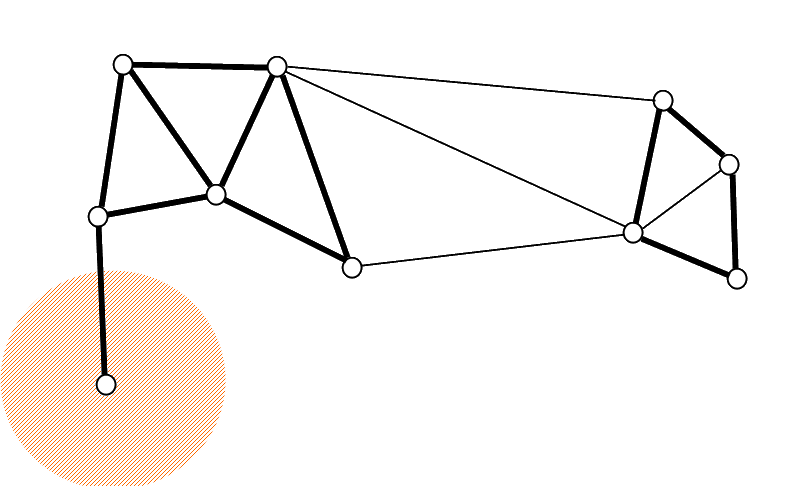
\includegraphics[width = 0.9\textwidth]{my_min_cut.png}
    \caption{Minimising the cut.}
  \label{fig:min_cut}
  \end{subfigure}
  \begin{subfigure}{0.4\textwidth}
    \centering
    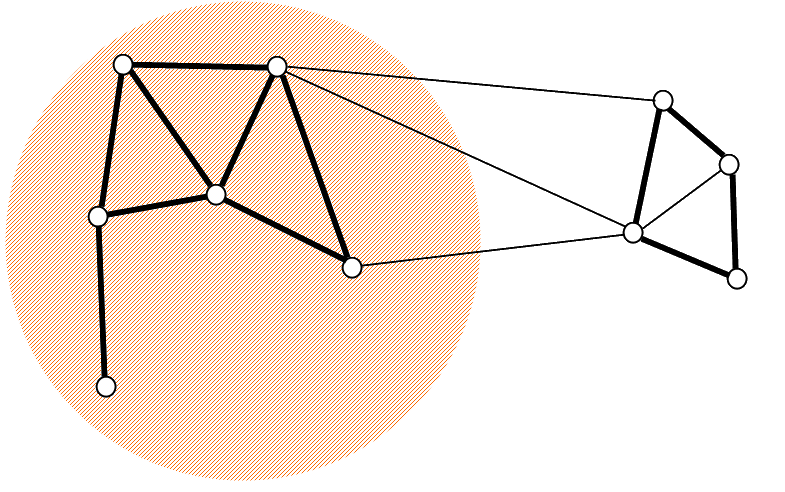
\includegraphics[width = 0.9\textwidth]{my_norm_cut.png}
  \caption{Minimising the normalised cut.}
  \label{fig:norm_cut}
  \end{subfigure}

  \caption{Two solutions to the bi partition problem. The partitioning is indicated by shading/non shading of nodes.}
  \label{fig:min_norm_cut}
\end{figure}


On Spectral Clustering \cite{Ng2001} was one of the first papers to provide theoretical guarantees on performance for spectral clustering algorithms.  Unlike previous authors who had only shown empirical results to justify spectral clustering abilities, they prove that their spectral clustering algorithm will produce a reasonable clustering, given certain assumptions that the clusters are well-spaced. This version of the spectral clustering algorithm has been popularly cited throughout the literature and is the one that we shall reference in Section \ref{sec:spec}. 

Although spectral clustering has been shown to perform well empirically on simple data sets, computational problems arise as the data set size increases. There have been a number of ways to deal with speed up in the static case, one of the most popular methods is to use Nystr\"{o}m efficiency methods ( \cite{Williams2001, Fowlkes2004}). The Nystr\"{o}m method samples the columns of the affinity matrix and approximates the full matrix by using correlations between the sampled columns and the remaining columns. Effectively we can think of this sampling as a dial which the user has control over. Sampling more columns will provide a better results but at a cost. Although Nystr\"{o}m methods are approximation techniques to speed up the computation of spectral clustering, the working memory can still be high. Another drawback with Nystr\"{o}m is that due to random sampling it is possible to under represent or entirely miss smaller clusters.  
One alternative to Nystr\"{o}m methods is to perform a permutation on the data to act as a pre-processing step to generate a smaller summary data set. By feeding a smaller set of representative points into the spectral clustering algorithm instead of the whole data set, we can lessen the effect of the computational bottleneck that comes with eigen analysis. Fast Approximate Spectral Clustering \cite{Yan2009}  explores the theoretical guarantees on misclustering the data set, given that some permutation has been performed on the data before the spectral clustering. Specifically they exactly quantify the misclustering of data sets, given that the original data is summarised using K-means (KASP) or a Random Project tree (RASP) as preprocessors. This is explored further in Section \ref{sec:spec}.

Another method to deal with the computational challenge in spectral clustering is Local Information-based Fast Approximate Spectral Clustering (Li-ASP) introduced in \cite{Cao2014}. Li-ASP consists of two upgrades; a sparse affinity graph to speed up computation and local interpolation to improve clustering performance. The sparse affinity graph uses a $k$ nearest neighbour or an $\epsilon$ neighbourhood to set many elements in the affinity graph to zero. Local interpolation is suggested based on an issue identified about KASP \cite{Yan2009} that if a representative point is miss-assigned to the wrong cluster, then all data points represented by that point will also be miss-assigned. Local interpolation can avoid these situations by using labelling data points with a weighted version of their $p$ closest representative points labels, rather than labelling based just on the label of the single closest representative point. 

One constant challenge in clustering is selecting the number of clusters to search for. \cite{Zelnik-Manor2004} present a method for automatically choosing the true number of clusters using the eigenvectors to inform their choice. More commonly the eigenvalues are used to estimate the number of clusters, but if the clusters are not clearly separated identifying the number of clusters from eigenvalues alone is not trivial. We shall assume that the true number of clusters is known. 

So far, we have only discussed spectral clustering of static data sets. We are interested in data streams, which are of great interest in today's world of communication graphs such as the Internet and social networks. Applications also include health care such as modelling epidemics and understanding sensor networks. Re-clustering the graph at each time step whenever new information arrives is not feasible especially if data is arriving rapidly.

To my knowledge, there is not currently a fully online method for Spectral Clustering. The problem of performing spectral clustering in data streams has been considered, but framed as an evolving network rather than a stream where data appears rapidly. Time evolving graphs are still an interesting problem, and are often found in social networks or biological applications. \RD{Sssht!}

\RD{Motivation/aims of this approach} The first incremental spectral clustering algorithm concerns topological mapping (\cite{Valgren2007}). Their algorithm updates the cluster estimates whenever a new data point (or batch of data points) arrives. The cluster membership is updated directly. The affinity matrix is periodically compressed to deal with large data sets. If a new data point is sufficiently far from its closest representative points, it is considered the start of a new cluster, this means that the number of overall clusters  must always increase. \RD{weakness}

An incremental update algorithm is proposed in \cite{Ning2007} and  \cite{Ning2010} which can deal with both additional data points joining the network, and similarity weights changing between existing data points. The algorithm updates the eigenvectors and eigenvalues directly without performing a full eigen-decomposition. The addition of a new data point is treated as a series of $n$ weight changes, where is $n$ is the number of currently observed data points.  However the authors recommend a full re-clustering in batch to minimise cumulative errors. There are some issues with update method, mainly that the updating of eigenvectors means that the orthogonality property may be lost.\RD{why is this an issue?} Also if the spatial neighbourhoods of often changing vertices are large it can still be computationally difficult as the eigenvector update step involves the inversion of a matrix. Finally the authors recommend a full spectral re-clustering occasionally to prevent the accumulation of errors in the eigenvectors, this is not feasible in the streaming setting. Generally this method is not suitable for data streaming, as the size of the Laplacian can grown unbounded for an infinite data stream. However since it is the most well-known relevant ``online'' algorithm existing, we will compare performance against it in Section \ref{sec:spec_clust_study}.  \RD{Might move Ning from experiments to \ref{sec:microSpec}}.

Other incremental spectral clustering algorithms include \cite{Kong2011}, \cite{Langone2014} and \cite{Dhanjal2011} which approximates the eigen decomposition of the Laplacian incrementally but still requires regular full re-clustering.\RD{Which is an issue because...}

%\Wu2014 \cite{Kannan2004} \cite{Guattery1998} \cite{Hagen1992} \cite{Jordan2004} \cite{Huang2009} \cite{Meila2001}  \cite{Pothen1990}  \cite{Stoer1997} \cite{Tibshirani2001} \cite{Luxburg2005} \cite{Luxburg2007} \cite{Wu2014} \cite{Zhang2014} 

We consider an online spectral clustering algorithm based on the Clustream model of \cite{Aggarwal2003}. The Clustream algorithm is introduced in full in Section \ref{sec:microSpec}, but first we discuss spectral clustering in more detail.

\section{Spectral Clustering}
\label{sec:spec}

In this Section we provide a brief introduction to Spectral Clustering, and discuss the choice of affinity matrices. A fast offline spectral clustering algorithm \cite{Yan2009} algorithm will be introduced, which inspired our implementation in Section \ref{sec:microSpec}.

The goal of clustering algorithms is to partition data ($\boldsymbol{X} =\boldsymbol{ x_1}, \boldsymbol{x_2}, \hdots, \boldsymbol{x_n}$, $\boldsymbol{x_i} \in \mathbb{R}^d$) into $k$ disjoint classes such that each $\boldsymbol{x_i} $ belongs to one and only one class. Clusters come in all shapes and sizes, they can be spherical and compact as in Figure \ref{fig:compact} or connected but not visually compact as in Figure \ref{fig:connected}. Data which is compact may be simple to cluster as the gaps between clusters are easy for simple clustering algorithms like k-means to identify. Connected but non-compact data sets are can be much more challenging than compact data sets, and can cause some simple clustering algorithms to fail. Spectral clustering can provide good quality segmentation on even these difficult cases, however its performance comes at the cost of computational complexity. We shall use the Jordan-Weiss (NJW) spectral clustering framework \cite{Ng2001} which is described in Algorithm \ref{alg:njw}. 

\begin{figure}[h!]
  \centering

  \begin{subfigure}{0.4\textwidth}
    \centering
    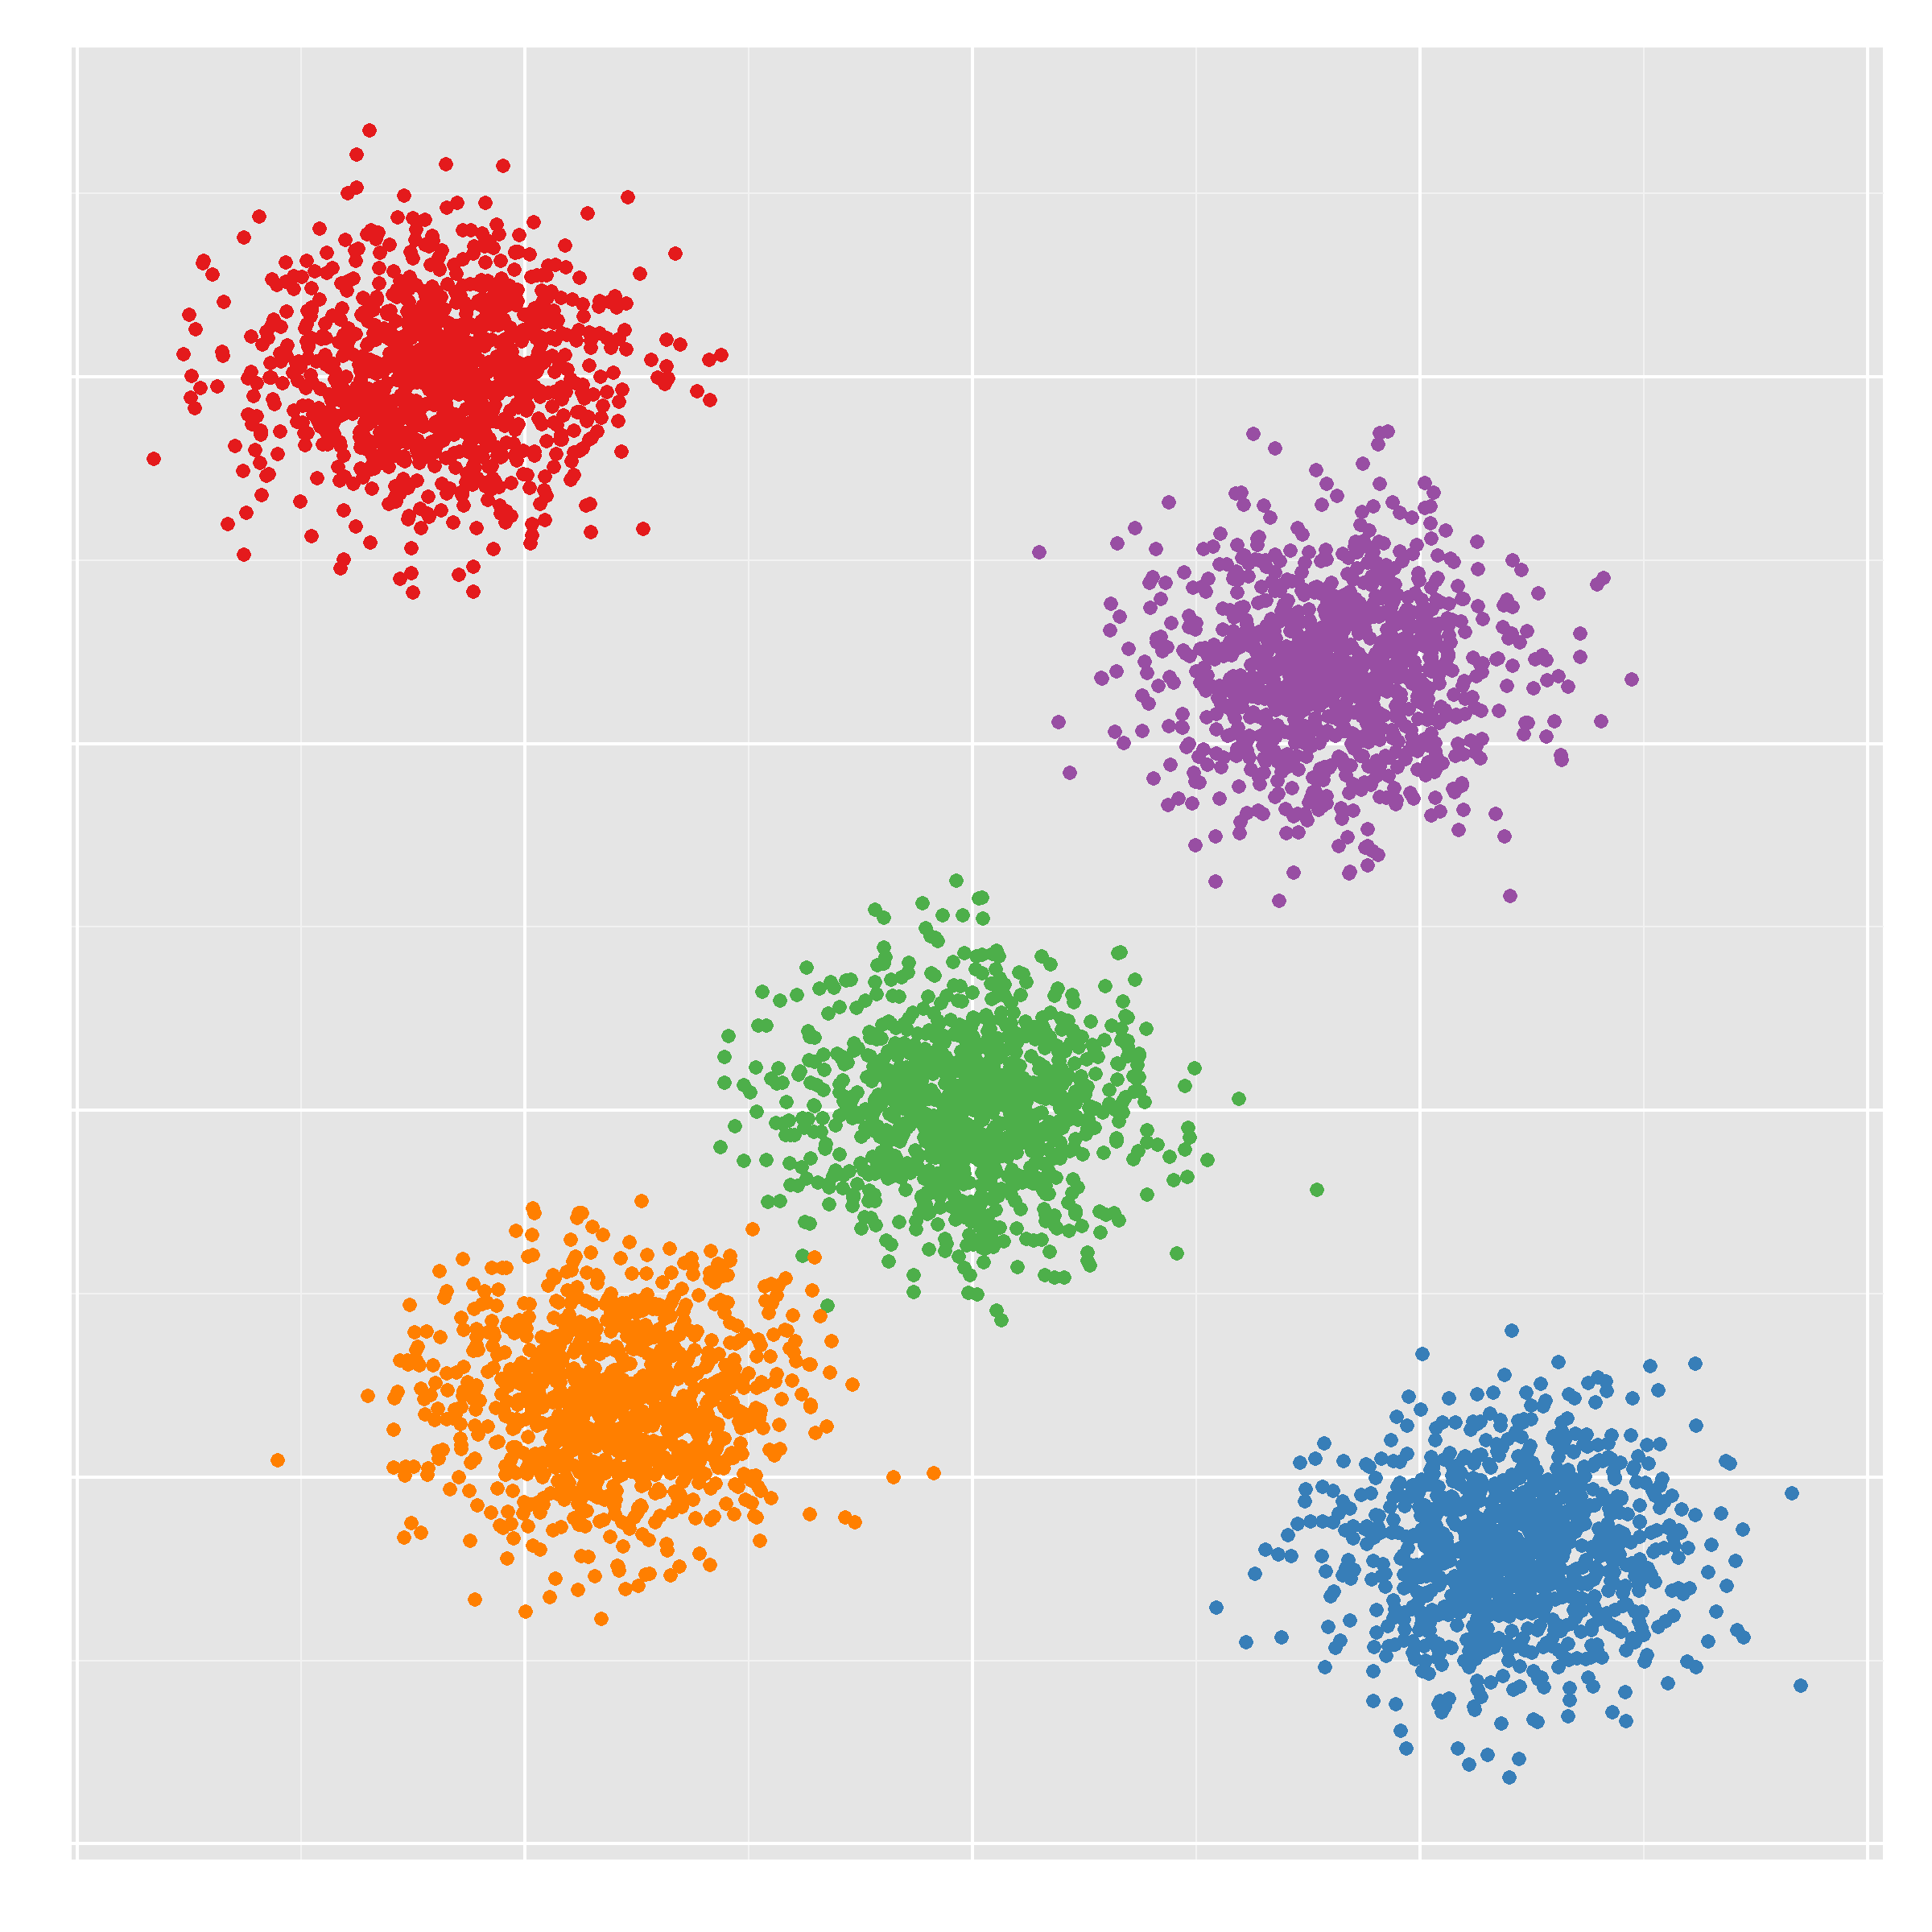
\includegraphics[width = 0.8\textwidth]{my_compact}
    \caption{Compact clusters}
  \label{fig:compact}
  \end{subfigure}
  \begin{subfigure}{0.4\textwidth}
    \centering
    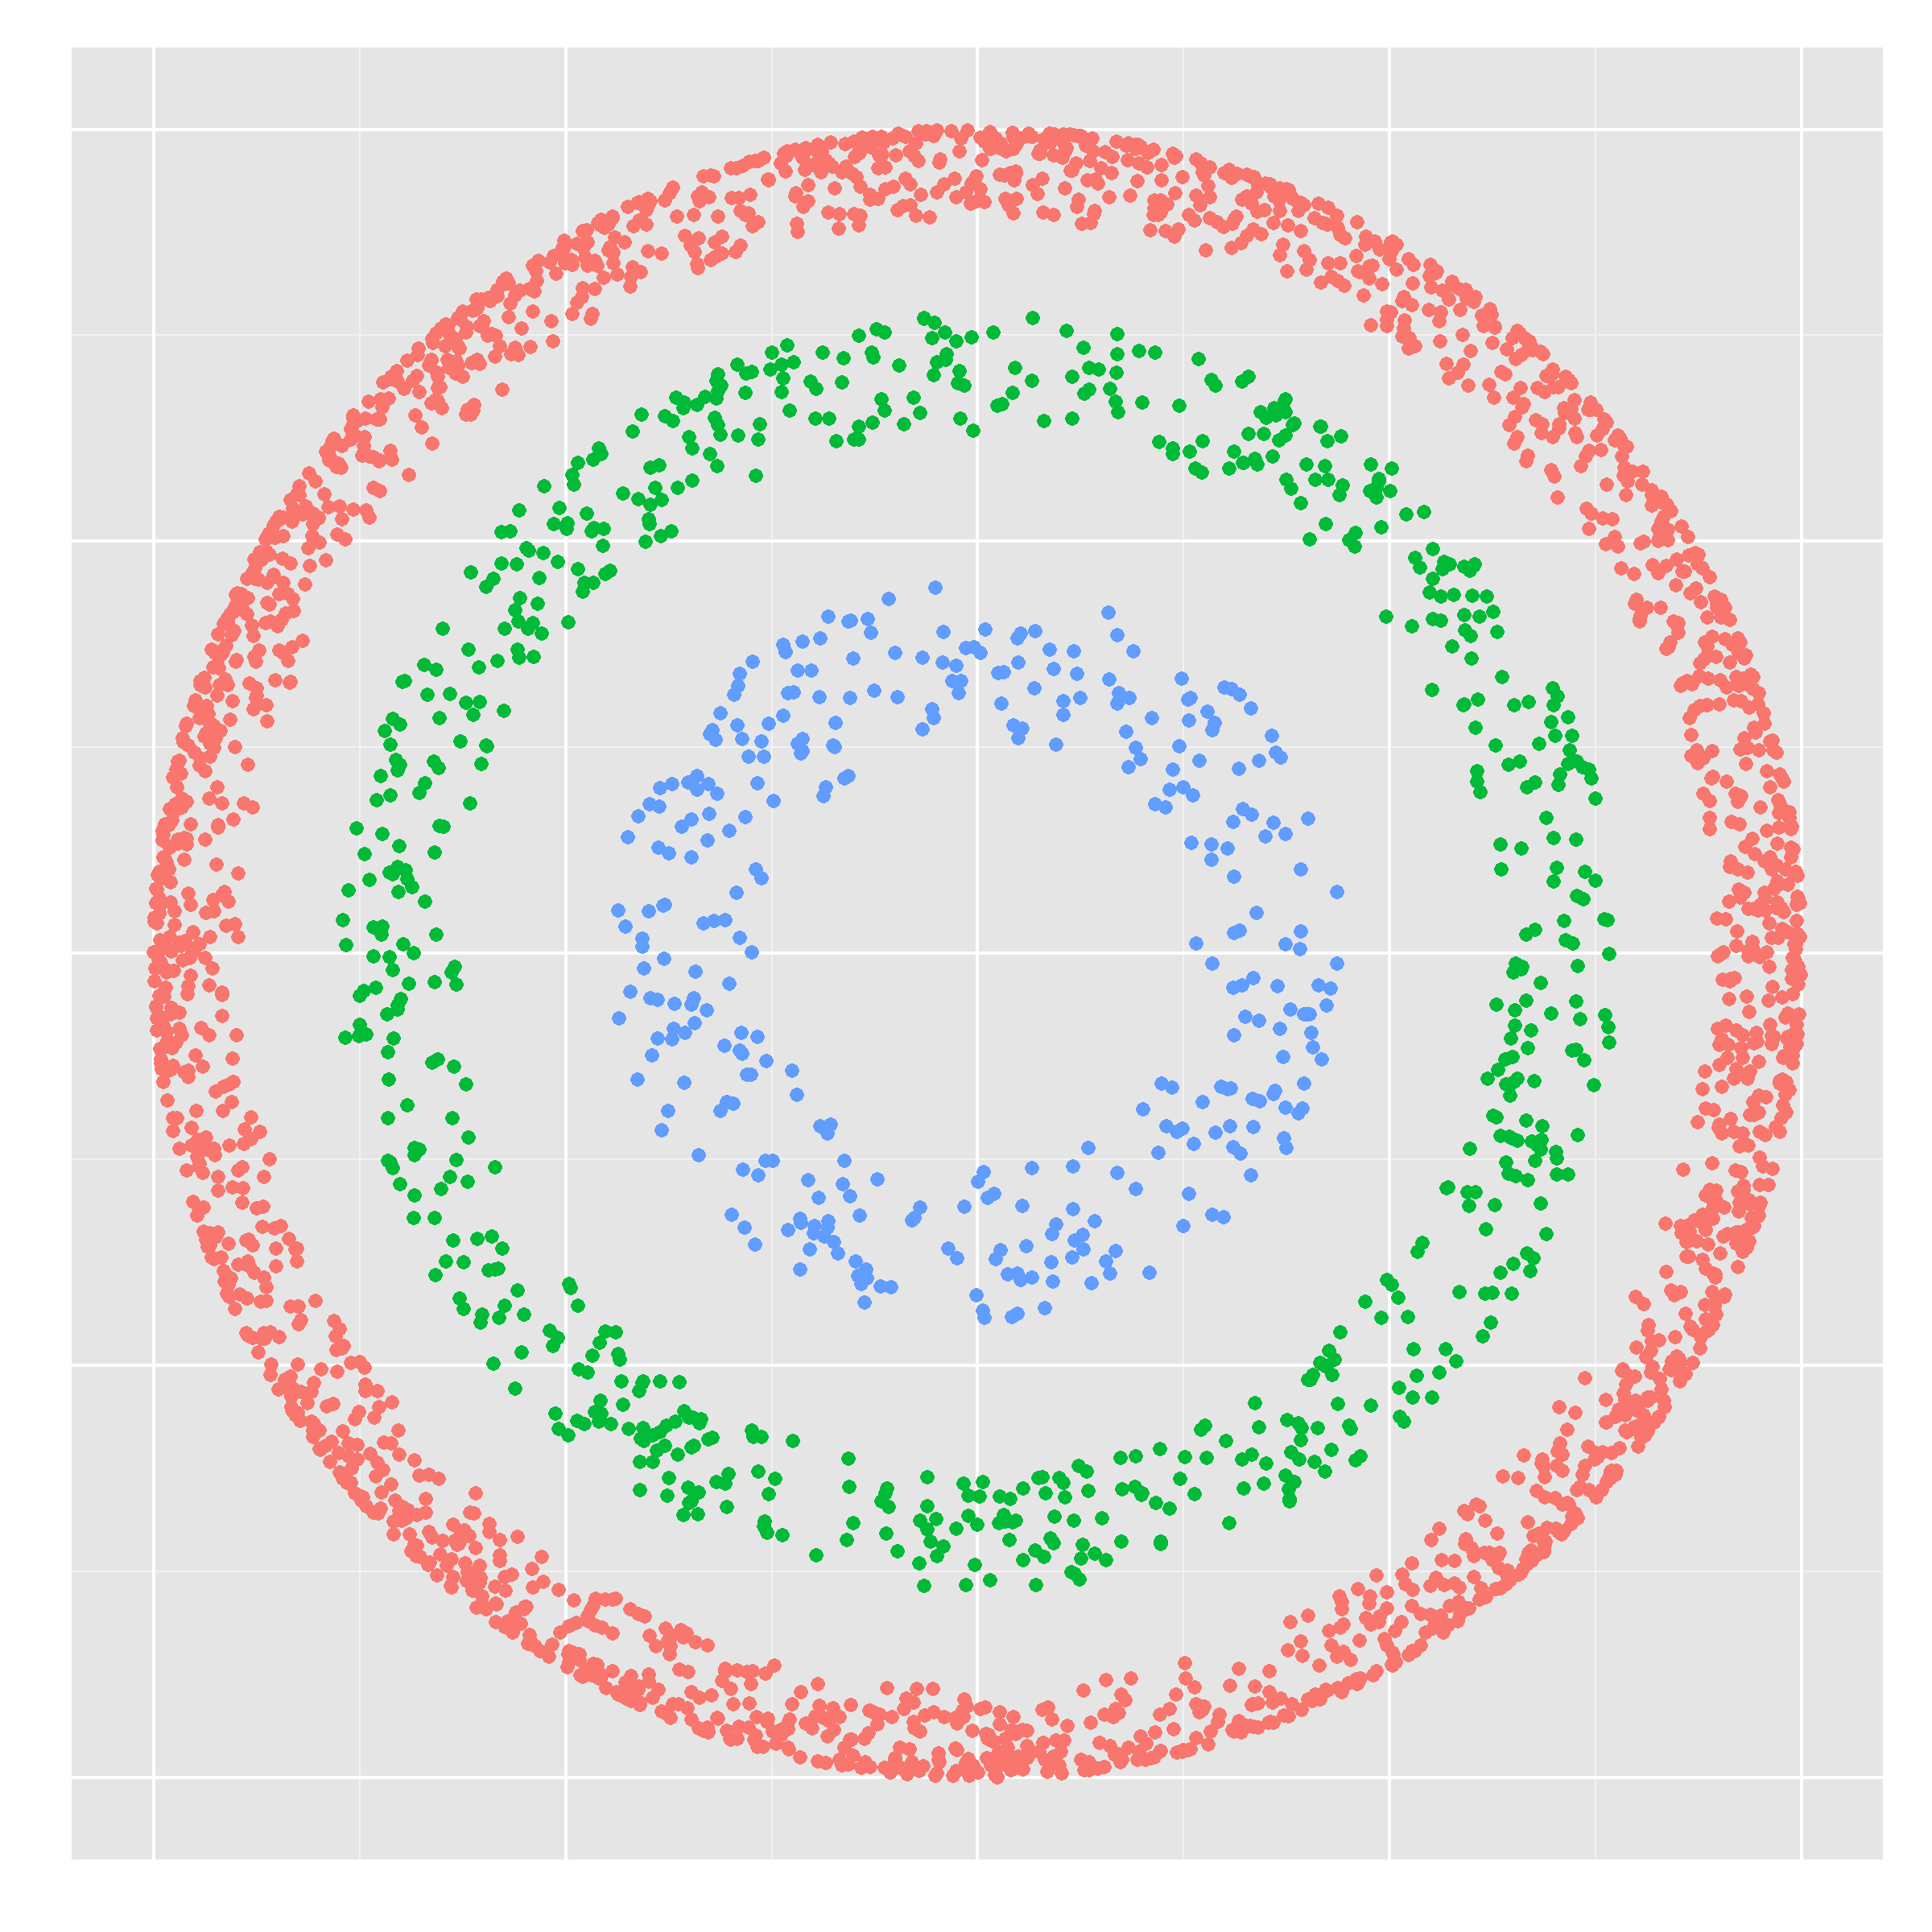
\includegraphics[width = 0.8\textwidth]{my_connected}
     \caption{Connected clusters}
     \label{fig:connected}
     \end{subfigure}
  \caption{Examples of different types of clusters}
  \label{fig:compact_connected}
\end{figure}

The affinity matrix $A = (a_{ij} )_{i,j = 1}^n$ represents the pairwise similarities or distances between all data points $x_i$ and $x_j$. A popular choice is to define $A$ to be the Gaussian kernel, as defined in equation \eqref{eq:gaussian_affinity}, where the parameter $\sigma$ controls the width of the local neighbourhoods which we want to model.

\begin{equation}
  \label{eq:gaussian_affinity}
    a_{i,j} = \exp  \left( - \frac{\| x_i - x_j \|^2}{2 \sigma^2} \right), i, j = 1, \ldots, n.
\end{equation}

 If $x_i$ and $x_j$ are very close, then $a_{i,j} \rightarrow 1 $, and if they are far apart $a_{i,j} \rightarrow 0$. A gaussian kernel affinity matrix will have ones along the diagonal and is symmetric $(a_{ij} = a_{ji})$.

The value scaling parameter $\sigma$  is usually chosen manually. \cite{Ng2001} automatically chose $\sigma$ by running their clustering algorithm repeatedly for a number of values and selecting the one which provides least distorted clusters. \cite{Zelnik-Manor2004} argue that for data which has a cluttered background, or multi-scale data, one global parameter choice for $\sigma$ is not sufficient. They calculate a localised parameter $\sigma_i$ for each data point $x_i$ based on it's neighbourhood. In our experimentation we did not find it necessary to do this and use a global $\sigma$. 

If we mainly wish to model the local relationships, using all of the possible pairwise data connections may not be necessary. It is possible to use a weighted k-nearest neighbour structure to build the affinity matrix once corrections have been made to ensure that this matrix is symmetrical. Another option is to choose some threshold $\epsilon$ and only consider connections between data points whose pairwise distances are smaller than $\epsilon$. This is an $\epsilon$-neighbourhood graph. Although it is possible to weight this graph by $\epsilon$, if we choose $\epsilon$ to generate a small $\epsilon$-neighbourhood, then the differences between the weights will be small that weighting may become eligible. Therefore a simple construction of the $\epsilon$-neighbourhood graph is as shown in equation \eqref{eq:epsilon_graph}. 

\begin{equation}
\label{eq:epsilon_graph}
  a^*_{ij}=\left\{
  \begin{array}{@{}ll@{}}
    1, & \text{if}\ a_{ij} < \epsilon \\
    0, & \text{otherwise}
  \end{array}\right.
\end{equation} 

Using this construction will give a sparse affinity matrix instead of a fully connected graph, which will help lower the computational complexity. In Section \ref{sec:spec_clust_study}, we use a fully connected graph for all experiments.\RD{Possibly KNN now} The degree of each vertex  is defined as, $d_i =\sum_{j = 1}^N A_{ij}$, the sum of the rows of the affinity matrix. The degree matrix, $D$, is then defined as a diagonal matrix with $i$\textsuperscript{th} diagonal element equal to $d_i$. We use the Normalised Symmetric Laplacian \citep{chung1997spectral} defined in equation \eqref{eq:norm_laplacian}, which relates to an approximation of minimising the Normalised Cut, discussed in Section \ref{sec:spec_lit}. \RD{Should I introduce unnormalised and random walk normalised too?} 

 \begin{equation}
   \label{eq:norm_laplacian}
   L=D^{-1/2}AD^{-1/2}
 \end{equation}

\RD{Would this be clearer if I explain unnormalised and state $L_{\text{symm}} = I - D^{-1/2}AD^{-1/2}$ }

\begin{algorithm}
\caption{NJW spectral clustering algorithm}
\begin{algorithmic}[1]
\REQUIRE Data set $X = {\boldsymbol{x_1},\ldots, \boldsymbol{x_n}  }$, number of clusters $k$
\ENSURE $k$-way partition of the input data
\STATE Construct the affinity matrix $A$ by the following Gaussian kernel function:
\begin{equation*}
  a_{i,j} = \exp  \left( - \frac{\| \boldsymbol{x_i} - \boldsymbol{x_j} \|^2}{2 \sigma^2} \right), i,j = 1, \ldots,n.
\end{equation*}

\STATE Compute the normalised affinity matrix $L = D^{-\frac{1}{2}}A D^{-\frac{1}{2}}$, where $D$ is the diagonal matrix with $D_{ii}=\sum_{j=1}^{n} a_{ij}.$
\STATE Compute the $k$ eigenvectors of $L$, $v_1, v_2,\ldots , v_k,$ associated with the $k$ largest eigenvalues, and form the matrix $ X = [\boldsymbol{v_1},\boldsymbol{v_2}, \ldots , \boldsymbol{v_k}]$.
\STATE Renormalize each row of $X$ to form a new matrix $Y$.
\STATE Partition the $n$ rows into $k$ clusters via a general cluster algorithm, such as the k-means algorithm.
\STATE Assign the original point $\boldsymbol{x_i}$ to the cluster $k$ $\iff$ the corresponding row $i$ of the matrix $Y$ is assigned to the cluster $k$.

\end{algorithmic}
\label{alg:njw}
\end{algorithm}

Spectral clustering can be challenging for very large data sets, constructing the affinity matrix $A$ and computing the eigenvectors of $L$ have computational complexity $\mathcal{O}(n^2)$ and $\mathcal{O}(n^3)$ respectively. A fast approximate spectral clustering algorithm is proposed (KASP) is proposed \cite{Yan2009} which uses a k-means pre processing step to lessen the computational complexity whilst retaining good clustering performance. Firstly k-means is run on the whole data set where $q$ is chosen to be large but such that $k \ll q$. The centres of the clusters are then used as representative data points for the whole data set. Spectral clustering is performed on the representative set only, which is significantly faster than performing spectral clustering on the full data set. The resulting cluster labels for the representative data are linked back to the original data set such that every original data point acquires the same label as its associated $k$-means cluster centre. The KASP algorithm is repeated in Algorithm \ref{alg:kasp} with unified notation.

\begin{algorithm}[h!]
\caption{KASP}
  \begin{algorithmic}[1]
   \REQUIRE Data set $X = {\boldsymbol{x_1},\ldots, \boldsymbol{x_n}  }$, number of clusters $k$, number of representative points $q$
   \ENSURE  $q$-way partition of the input data
   \STATE Perform k-means with $q$ clusters on $\boldsymbol{x_1}, \hdots, \boldsymbol{x_n}$
   \STATE Compute the cluster centroids $y1, \hdots, y_q$ as the $q$ representative points.
   \STATE Build a correspondence table to associate each $x_i$ with the nearest cluster centroids $y_j$ .
   \STATE Run a spectral clustering algorithm on $y_1,\hdots, y_q$ to obtain an $k$-way cluster membership
   for each of $y_q$.
   \STATE Recover the cluster membership for each $x_i$ by looking up the cluster membership of the corresponding centroid $y_j$ in the correspondence table.
  \end{algorithmic}
\label{alg:kasp}
\end{algorithm}

The KASP algorithm has been shown to perform well empirically, and using representative points is a sensible way to lessen the computational burden. As the number of representative points increases, the better performance should be, but the greater the computational expense. 

In online spectral clustering algorithm, we will use representative points as an input for spectral clustering. Rather than  generating representative points from a k-means step, we  constantly update the representative points by using the streaming algorithm, Clustream which is introduced in Section \ref{sec:microSpec}.


\section{Micro-cluster based spectral clustering in data streams}
\label{sec:microSpec}

In this Section we discuss online streaming methods, introduce the streaming algorithm Clustream, and consider how to use incorporate the streaming data into a spectral clustering algorithm.

\subsection{The challenges of clustering data streams}

A relatively new challenge to clustering is working with data streams \cite{Gama2010, Silva2013}. A data stream is data which arrives in an ordered sequence, continuously; for example, sensor data or online shopping transactions. There is no control over the order in which data objects should be processed. A data stream may be potentially unbounded, and the data points are often discarded after processing.  Much work has been done developing offline clustering methods, such as spectral clustering, but it is not suitable to apply these offline methods directly to the streaming scenario. Simply running an offline clustering algorithm on all the data observed so far may not be feasible for three main reasons, storage capacity, computational costs and ability to access to the data.

The first challenge is storing all of the data. As a data stream is a potentially an endless sequence of observations obtained at a high frequency often, it may not be possible to store all of the data in its entirety. Therefore the older data has to be thrown away to make room for the new arrivals. This might not seem like a big issue as the data will naturally become weighted temporally, but this is challenging if we wish to incorporate historical data into the clustering.

Secondly, as we have discussed, clustering algorithms can be computationally expensive. For example, computing the eigenvectors for spectral clustering has complexity $\mathcal{O}(n^3)$. As data streams are potentially unbounded, standard clustering algorithms cannot be used.  Therefore we need to be able to update our idea of the data as new points arrive efficiently and simply with little computational issues.

Finally, data streaming is often classed as a ``one-pass-access'' problem. Imagine a constant stream of data flying past your window, you can view the data as it flies by the window, but once it has passed by, it cannot be accessed again. Some traditional clustering algorithms such DBScan (\cite{Ester1996}) require many passes or iterations of the data, therefore these type of clustering methods are not directly suitable for the online data streaming case.
 
\subsection{Clustream}

Clustream \cite{Aggarwal2003} offers a framework which allows quick and easy updates and the ability to perform sophisticated clustering algorithms. Clustream has proved popular, since the paper was first published in 2003 it has been cited over 1400 times. The main idea is to separate the clustering process in two stages, a micro-clustering stage and a macro-clustering stage. The  micro-clustering stage continuously updates statistical summaries of the data stream, and the macro-clustering is more computationally intensive and run in batch or on a user request. 

\subsubsection{Micro-clustering}

The micro-clustering stage is a way of maintaining an active, evolving representative summary of the data, without storing the absolute values of the data points. Micro-clusters are defined as a temporal extension of the cluster feature vector first described in \cite{Zhang1996a}. The data stream is summarised by many small clusters, which are initially generated by $k$-means. The online phase stores $q$ micro-clusters in memory, where $q$ is an input parameter.
We take an initial training set, and perform k-means with $q$ clusters but choose the value of $q$ to be much larger than the expected number of true macro-clusters $k$, $(k \ll q)$. The aim here is to create a fine scale summary of the data. The value of $q$ should be chosen to be as large as computationally comfortable. The larger $q$ is, the finer scale that the summaries will be. It is vital to ensure that the micro-cluster well represent the underlying data set or else the macro-clustering will under perform. These $q$ clusters are our first micro-clusters. Over time, we will update these micro-clusters, adding new data points to them, merging them and removing old micro-clusters, although the number of micro-clusters should stay fixed throughout. 

The micro-clusters can then be used on a user request to perform a macro-clustering using the summarised data rather than the full data set. If the micro-clusters represent the true underlying data stream well, then the difference between the clustering on the summarised data and the true full data should be small. 

Assume that we have a data stream $S$ which consists of $d$-dimensional data $\boldsymbol{x_i}$ arriving in sequence. $S = \{\boldsymbol{ x_1}, \boldsymbol{x_2}, \boldsymbol{x_3}, \hdots \boldsymbol{x_i}, \hdots, \}, \boldsymbol{x_i} \in \mathbb{R}^d$. Each micro-cluster $M_j$ for $(j \in 1 \ldots, q)$ is stored as a ($2 \cdot d + 3$) tuple $(\boldsymbol{CF1^x_j}, \boldsymbol{CF2^x_j}, n_j, CF1^t_j, CF2^t_j)$. The definitions are given in equation \eqref{eq:microcluster_def}. $\boldsymbol{CF1^x_j}$ is the sum of all observed data in that micro-cluster, $\boldsymbol{CF2^x_j}$ is the sum of the squares of the data and $n_j$ is the number of elements assigned to that micro-cluster. $CF1^t_j$ and $CF2^t_j$ refer to the sum of the time stamps, and the sum of squared time stamps respectively. Note that both $\boldsymbol{CF1^x_j}$ and $\boldsymbol{CF2^x_j}$ are $d$-dimensional vectors.

Each micro-cluster $M_j$ will have 
\begin{align}
\boldsymbol{CF1^x_j} &= \quad \sum_{x_i \in M_j}{\boldsymbol{x_i}} \; , \nonumber  \\ 
\boldsymbol{CF2^x_j} &= \quad \sum_{x_i \in M_j}{(\boldsymbol{x_i})^2} \; , \nonumber\\
CF1^t_j &= \quad \sum_{i | x_i \in M_j}{t_i} \; , \nonumber   \\
CF2^t_j &= \quad\sum_{i | x_i \in M_j}{(t_i)^2} \; , \nonumber\\
n_j &= \quad \sum_{x_i \in M_j}{1} \; .
\label{eq:microcluster_def}
\end{align}

If a new data point $x_{\text{new}}$ arrives at time $t_{\text{new}}$ and is assigned to micro-cluster $M_j$, the  update  given in equation \eqref{eq:microcluster_update} is applied. 
\begin{align}
\boldsymbol{CF1^x_j} \quad &\leftarrow \quad \boldsymbol{CF1^x_j} + \boldsymbol{x}_{\text{new}} \; , \nonumber  \\ 
\boldsymbol{CF2^x_j} \quad &\leftarrow \quad \boldsymbol{CF2^x_j} + (\boldsymbol{x}_{\text{new}})^2 \; , \nonumber\\
CF1^t_j \quad &\leftarrow \quad  CF1^t_j + t_{\text{new}} \; , \nonumber   \\
CF2^t_j \quad &\leftarrow \quad CF2^t_j + (t_{\text{new}})^2 \; , \nonumber\\
n_j  \quad &\leftarrow \quad n_j + 1 \; .
\label{eq:microcluster_update}
\end{align}

Note that updating the micro-clusters requires only addition therefore updating is cost effective. Critically it is possible to use these summaries to calculate the centre of each micro-cluster as in equation \eqref{eq:micro_centre}. It is these centres which as used as representative points for input into the macro-clustering.  As new points in the data stream arrive, they are either allocated to a micro-cluster and the update procedure discussed above is carried out, or a new micro-cluster is created. The decision for a new micro-cluster to be created is based on whether the new data point is close enough to it's nearest cluster centre. 

\begin{equation}
  \label{eq:micro_centre}
  \text{Centre of micro-cluster j}  = \boldsymbol{\bar{M_j}} = \frac{\boldsymbol{CF1^x_j}}{n_j}
\end{equation}

When a new data point arrives it's nearest micro-cluster $M_{*}$ is identified using the Euclidean distance metric given in equation \eqref{eq:m*}. If the data point falls within the Maximum Boundary Factor of it's nearest cluster centre, then it is absorbed as part of that cluster. If not, it is used to create a new micro-cluster. However we stated earlier than the number of micro-clusters must remain fixed throughout the process. Therefore if a new micro-cluster is formed, either an existing  micro-cluster must be deleted, or two close micro-clusters should be merged. We follow the methodology in Clustream by first looking for an old micro-cluster to delete using the time-stamp references detailed in the original paper and otherwise combine the two nearest micro-clusters. In this way, the algorithm tracks the data stream as it evolves. 

\begin{equation}
  \label{eq:m*}
 M^{*} = \argmin_{M_j , j \in 1:q} \lVert {\boldsymbol{x_i} -\boldsymbol{\bar{M_j}} } \rVert ^2
\end{equation}

In Clustream, the maximum boundary factor is defined as a factor of $t$ of the RMS deviation of the data points in $M_j$ from the centroid of $M_j$. The RMS deviation can only be defined for a cluster with more than one point. For a cluster with only one previous point, a heuristic is used to define the MBF. Details of the MBF can be found in \cite{Aggarwal2003}% \RD{Paper uses r times that of the next closest cluster. Should I write MBF mathematically? Maybe show it visually with the cuboids.}

With this online micro-cluster maintenance, the data stream should remain well represented over time. When a new data point arrives if it is the start of a new evolving cluster it will be allowed to grow however if it is an outlier no more points will be added to it and over time it may be deleted from the system all together.

If two micro-clusters $M_r$ and $M_s$ are to be merged, the updates given in equation \eqref{eq:microcluster_merge} are used to merge them into $M_r$, and $M_s$ will be deleted. Again as all of these updates only involve addition steps, they are fast to implement. 
\begin{align}
\boldsymbol{CF1^x_r} \quad &\leftarrow \quad \boldsymbol{CF1^x_r} + \boldsymbol{CF1^x_s} \; , \nonumber  \\ 
\boldsymbol{CF2^x_r} \quad &\leftarrow \quad \boldsymbol{CF2^x_r} + \boldsymbol{CF2^x_s} \; , \nonumber\\
CF1^t_r \quad &\leftarrow \quad  CF1^t_r + CF1^t_s\; , \nonumber   \\
CF2^t_r \quad &\leftarrow \quad CF2^t_r +  CF2^t_s\; , \nonumber\\
n_r  \quad &\leftarrow \quad n_r + n_s \; .
\label{eq:microcluster_merge}
\end{align}

The micro-clustering update algorithm for Clustream is given in Algorithm \ref{alg:onlineSpec}.

\begin{algorithm}
\caption{Clustream Microclustering}  
\begin{algorithmic}
\REQUIRE Data Stream $S = {\boldsymbol{x_1},\ldots, \boldsymbol{x_n}  }$, number of micro-clusters $q$
\ENSURE Microclusters $M_1, \ldots, M_q$
\STATE Initialise the micro-clusters kmeans($x_1, \hdots x_{init},q$) and equations \eqref{eq:microcluster_def}
\FOR {each new data point $x_i$}
 \STATE Find the closest micro-cluster to $x_i$, $M_*$ using equation \eqref{eq:m*}
 \IF{$x_i$ satisfies the MBF criterion for $M_*$ }
   \STATE absorb $x_i$ into micro-cluster $M_*$ using equations \eqref{eq:microcluster_update}
 \ELSE
 \STATE Use $x_i$ to initialise it's own new micro-cluster using equations \eqref{eq:microcluster_def}
  \IF{any micro-cluster is suitably old}
   \STATE Remove it
  \ELSE 
   \STATE Merge the two closest micro-clusters using equation \eqref{eq:microcluster_merge}
  \ENDIF
\ENDIF
\ENDFOR
\end{algorithmic}
\label{alg:clustream}
\end{algorithm}
%Thus, the CluStream algorithm finds the arrival time (known as the relevance time) of the m/(2Ni)th percentile of the Ni objects in a micro-cluster i, whose timestamps are assumed to be normally distributed.
\subsubsection{Macro-clustering stage}
 
The second stage of clustream is a macro-clustering stage, where we take the current micro-cluster feature vectors, and use these as input into global clustering algorithm. The macro-clustering step is where the general data summary is transformed into a snapshot of the true underlying clusters at that point in the stream. The $q$ micro-cluster centres $\bar{M_j},(1 \leq j \leq q$) are treated as representative points for the data stream $S$, and a standard clustering algorithm can be used to determine clusters. The nature of this algorithm allows the user to get close to online streaming and perform spectral clustering on a summary of the whole of the data set. The full algorithm is given in Algorithm \ref{alg:onlineSpec}.

There are a number of possible ways to feed the micro-clusters into a spectral clustering algorithm. Two of the options suggested in \cite{Zhang1996a} are implemented here. 

\begin{enumerate}
\item Calculate the centre of each micro-cluster $\bar{M_j}$ and use it as an object to be clustered by the macro-clustering algorithm.
\item Do the same as before, but weighting each micro-cluster centre $\bar{M_j}$ proportionally to $n_j$, the number of points assigned to that micro-cluster, so that micro-clusters with more objects will have more influence on the final clustering.
\end{enumerate}


%In order to achieve this we adopt a micro-clustering type approach to quickly update a summary of the data. When an overall clustering is required, spectral clustering is performed using the centres of the micro-clusters as the input data. The micro-clusters act as a way of summarising the constantly arriving data steam whilst allowing updates to occur in a non intrusive, non-computationally difficult man8888888888888888888888888888888888888888888888888888888888888888888888888888888888888888888888888888888888888888888888888888888888888888888888888888888888888888888ner, with limited storage requirements. 

\begin{algorithm}
\caption{Online Spectral Clustream}
\begin{algorithmic}[1]
\REQUIRE Data Stream $S = {\boldsymbol{x_1},\ldots, \boldsymbol{x_n}  }$, number of clusters $k$, number of micro-clusters $q$
\ENSURE A $k$ way clustering of the microclusters $M_1, \ldots, M_q$.
\STATE Initialise the micro-clusters kmeans($x_1, \hdots x_{init},q$) and equations \eqref{eq:microcluster_def}
\FOR {each new data point $x_i$}
 \STATE Apply Clustream update as in Algorithm \ref{alg:clustream}
 \IF{A Macro-clustering is required}
   \STATE Perform spectral clustering on $M_1, \ldots, M_q$ with $k$ clusters.
\ENDIF
\ENDFOR

\end{algorithmic}
\label{alg:onlineSpec}
\end{algorithm}

In Section \ref{sec:spec_clust_study} we analyse the performance of both unweighted and weighted Online Spectral Clustering, but first we further investigate how to use weighted micro-clusters in Spectral Clustering.

\subsection{Weighting the Micro-Clusters}

In this section, we discuss how can create a weighted affinity matrix, look at the effect this has on the Laplacians, and note a spectral link between weighting in this manner, and a larger affinity of repeated points.

Why would it be beneficial to weight micro-clusters? For example Figure \ref{fig:microHist} shows how the distribution of points to microclusters may change as the stream progresses. Figure \ref{fig:hist1} shows a histogram of the number of points assigned to micro-clusters at the start of the stream, Figure \ref{fig:hist2} shows the middle of the stream, and Figure \ref{fig:hist3} shows the end of the stream. We can see that the distribution is not uniform. Therefore some information is contained in the number of points assigned to a micro-cluster. 

\begin{figure}[h!]
  \centering
  \begin{subfigure}{0.3\textwidth}
    \centering
    
\includegraphics[width = \textwidth]{missing.png}
    \caption{Start of the stream}
  \label{fig:hist1}
  \end{subfigure}
  \begin{subfigure}{0.3\textwidth}
    \centering
    
\includegraphics[width = \textwidth]{missing}
  \caption{Middle of the stream}
  \label{fig:hist2}
  \end{subfigure}
\begin{subfigure}{0.3\textwidth}
    \centering
    
\includegraphics[width = \textwidth]{missing}
  \caption{End of the stream}
  \label{fig:hist3}
  \end{subfigure}
    \caption{CREATE PLOTS Histograms showing the number of points assigned to microclusters}
  \label{fig:microHist}
\end{figure}


In order to weight the the micro-clusters, we simply construct an affinity as described. 
Let $A \in \mathbb{R}^{q \times q}$ be the affinity matrix of the micro-cluster centres with $i,j$-th element equal to the similarity between micro-cluster $M_i$ and $M_j$, 

\[ A_{i,j} = \exp \left(- \frac{\| \bar{M_i} - \bar{M_j}\|^2}{2 \sigma^2} \right), \quad i, j = 1, \ldots, q. \].

Let $\tilde{A} \in \mathbb{R}^{q \times q}$ have $i,j$-th element equal to $n_in_jA_{ij}$. $\tilde{A}$ is a valid affinity matrix since it is symmetric with non-negative entries. If we wish to have $\tilde{A}_{ij} \leq 1$ then simply divide $\tilde{A}$ by $max_i n_i^2$, but this makes no difference to the spectral decomposition. 

There exists a link between the spectral decomposition of  the Laplacian generated by $\tilde{A}$ and the Laplacian arising from a data set of repeated points, which we define as follows.  Let $A^* \in \mathbb{R}^{n \times n}$ be the repeated affinity matrix with the micro-cluster centres repeated based on the number of points assigned to them. Assume that the columns (and therefore rows) of $A^*$ are ordered such that the first $n_1$ are associated with the data assigned to micro-cluster 1, which has size $n_1$ and the next $n_2$ with those assigned to micro-cluster 2, and so on.

Let $D, \tilde{D}, D^{*},$ be the corresponding degree matrices and $L, \tilde{L}, L^{*}$ be the corresponding normalised symmetric Laplacians.

Lets look at the Affinity and Laplacian matrices more closely for a very simple case. 

Assume we have two micro-clusters, $M_1$ and $M_2$,  which have $n_1$ and $n_2$ points assigned to them respectively. Let the similarity between the two micro-clusters centres be $s$, and assume that we are using the standard Gaussian kernel to generate affinity matrices, so therefore the diagonal elements will be equal to 1. 

\[ A = \left(
  \begin{array}{cc}
    1 & s \\
    s & 1
  \end{array} \right), \quad
%
 D = \left(
  \begin{array}{cc}
    1+s & 0 \\
    0 & 1+s
  \end{array} \right), \quad
%
 L_{\text{symm}} = \left(
  \begin{array}{cc}
    \frac{1}{1+s} & \frac{s}{1+s} \\
    \frac{s}{1+s} & \frac{1}{1+s} 
  \end{array} \right) \]

In order to create a weighted version of the affinity matrix, we simple multiply through by $n_1$ and $n_2$. We can see how this is incorporated into the Laplacian. Note that we are working with the Symmetric Normalised Laplacian. In order to weight in this manner for the unnormalised Laplacian a scaling of the diagonal matrix is required.  

\[ \tilde{A} = \left(
  \begin{array}{cc}
    n_1^2 & sn_1n_2 \\
    sn_1n_2 & n_2^2
  \end{array} \right) , \quad
%
 \tilde{D} = \left(
  \begin{array}{cc}
    n_1^2 + sn_1n_2 & 0 \\
    0 & n_2^2 + sn_1n_2
  \end{array} \right) \]

\[
 \tilde{L}_{\text{symm}} = \left(
  \begin{array}{cc}
   \frac{n_1^2}{n_1^2+sn_1n_2} & \frac{sn_1n_2}{\sqrt{(n_1^2+sn_1n_2)(n_2^2+sn_1n_2)}} \\
   \frac{sn_1n_2}{\sqrt{(n_1^2+sn_1n_2)(n_2^2+sn_1n_2)}} &  \frac{n_2^2}{n_2^2+sn_1n_2}
  \end{array} \right) \]

Now lets look at the repeated affinity matrix. Here we can see the block nature in $A^*$, $D^*$ and $L^*$.

\[ A^* = \left(
  \begin{array}{cccccc}
    1 & \hdots & 1 & s & \hdots & s \\
    \vdots & \ddots & \vdots & \vdots & \ddots & \vdots \\
    1 & \hdots & 1 & s & \hdots & s \\
   s & \hdots & s & 1 & \hdots & 1 \\
    \vdots & \ddots & \vdots & \vdots & \ddots & \vdots \\
    s & \hdots & s & 1 & \hdots & 1 
  \end{array} \right) , \quad
%
 D^* = \left(
  \begin{array}{cccccc}
    \star & 0 & 0 & 0 & \hdots & 0 \\
    0 & \ddots & 0 & \vdots & \ddots & \vdots \\
    0 & 0 & \star & 0 & \hdots & 0 \\
   0 & \hdots & 0 & \bigtriangleup & 0 & 0 \\
    \vdots & \ddots & \vdots & 0 & \ddots & 0 \\
    0 & \hdots & 0 & 0 & 0 & \bigtriangleup 
  \end{array} \right) \]

where $\star = n_1 + n_2s$ and $\bigtriangleup = n_1s + n_2$.

\[ L_{\text{symm}}^* = \left(
  \begin{array}{cccccc}
    \frac{1}{\star} & \hdots & \frac{1}{\star} & \frac{s}{\sqrt{\star \bigtriangleup}} & \hdots & \frac{s}{\sqrt{\star \bigtriangleup}} \\
    \vdots & \ddots & \vdots & \vdots & \ddots & \vdots \\
    \frac{1}{\star} & \hdots & \frac{1}{\star} & \frac{s}{\sqrt{\star \bigtriangleup}} & \hdots & \frac{s}{\sqrt{\star \bigtriangleup}} \\
   \frac{s}{\sqrt{\star \bigtriangleup}} & \hdots & \frac{s}{\sqrt{\star \bigtriangleup}} & \frac{1}{\bigtriangleup}  & \hdots &  \frac{1}{\bigtriangleup} \\
    \vdots & \ddots & \vdots & \vdots & \ddots & \vdots \\
    \frac{s}{\sqrt{\star \bigtriangleup}} & \hdots & \frac{s}{\sqrt{\star \bigtriangleup}} & \frac{1}{\bigtriangleup}  & \hdots &  \frac{1}{\bigtriangleup} 
  \end{array} \right) \]

If we evaluate these expressions for a particular case, we can see how the spectral decomposition of the matrices are linked.

Let $s = 0.5$, $n_1 = 3$, $n_2 = 2$.

The 2nd smallest eigenvector of $L^*_{\text{symm}}$ is 
\[ e_2^* = \left[ 
\begin{array}{ccccc}
  -0.350& -0.350& -0.350& 0.562& 0.562  
\end{array} \right]
\]

The 2nd smallest eigenvector of $\tilde{L}_{\text{symm}}$ is 
\[ \tilde{e}_2 = \left[ 
\begin{array}{cc}
  0.607 & -0.795 \\
\end{array} \right]
\]

If we expand the eigenvector $\tilde{e}_2$ by repeating it's elements and block divide by $\sqrt{n_1}$ and $\sqrt{n_2}$ respectively, we get

\[ \left( \overbrace{\frac{0.607}{\sqrt{3}} \; \frac{0.607}{\sqrt{3}} \; \frac{0.607}{\sqrt{3}}}^{n_1} \; \overbrace{\frac{-0.795}{\sqrt{2}} \; \frac{-0.795}{\sqrt{2}}}^{n_2} \right) 
=  \left( 
\begin{array}{ccccc}
0.350& 0.350& 0.350 & -0.562& -0.562  
\end{array} \right)
\]

which is the negative of the 2nd smallest eigenvector of $L^*_{\text{symm}}$, $e_2^*$. 
In fact, we will always have that the expanded repeated eigenvector of the weighted Laplacian equal to either $e_k^*$ or $-e_k^*$ for all $k$.

We can see more generally that, \RD{What can we say generally?!}

Let $\tilde{u}$ be the second smallest eigenvector of $\tilde{L}$.

Define $u^* =  \left( \overbrace{\frac{\tilde{u}_1}{\sqrt{n_1}}, \; \frac{\tilde{u}_1}{\sqrt{n_1}}, \; \frac{\tilde{u}_1}{\sqrt{n_1}}}^{n_1}, \; \hdots, \overbrace{\frac{\tilde{u}_k}{\sqrt{n_k}}, \; \frac{\tilde{u}_k}{\sqrt{n_k}}}^{n_k} \right)$. 

We can see that $\|u^*\|^2 = \sum_{i = 1}^{n}(u_i^*)^2 = \sum_{i=1}^{k}n_i \cdot \frac{\tilde{u}_i^2}{n_i} = \sum_{i = 1}^{k} \tilde{u}^2_i = 1$. 

\section{Experimentation}
 \label{sec:spec_clust_study}

In the experimentation section, we investigate the performance of Spectral Clustream, both unweighted and weighted variants, along with a simple windowed approach. 


\subsubsection{The Algorithms}

Spectral Clustream is our implementation of Algorithm \ref{alg:clustream}. As highlighted in Section \ref{sec:microSpec}, there are two  ways we can incorporate the micro-cluster centres into the macro-clustering. Unweighted clustream takes the micro-cluster centres as direct input into the spectral clustering algorithm. Weighted clustream weights the micro-cluster centres by the number of data points assigned to that micro-cluster. In both clustream algorithms, we use 150 micro-clusters to monitor the streams.

Windowed Spectral Clustering is a simple algorithm stores a window of size $w$ of the most recently observed data points. When a new data point is observed, the oldest data point in the window is discarded to make room for the new data point. Only the data points in the current window are available for input into a standard Spectral Clustering algorithm. We use a fixed window size of $150$ data points for the duration of the stream.

%\subsubsection{Incremental Spectral Clustering}
%\RD{Recap Ning algorithm.} Not using in current experiments atm due to big speed issues. See Section \ref{sec:exp_ning}.Discuss the need to re-cluster regularly (how can we cope with this in a streaming setting?)Settings for experiments: Empirically we found (like the authors) that 2 iterations of the update step is enough to stabilise the estimates of the eigenvalues and eigenvectors and use that setting. 

\subsection{Methodology}
\label{sec:methodology}

A simulated data stream $S = {\boldsymbol{x_1},\ldots, \boldsymbol{x_n}  }$ is observed sequentially, with one data point $\boldsymbol{x_t}$ observed at each time point $t \in 1, \ldots, n$. Clustream requires the micro-clusters to be initialised. We do this by applying kmeans with 150 clusters to the first 500 points. The initial micro-cluster components are then calculated using the equations described in equation \eqref{eq:microcluster_def}. Spectral Windowed uses $150$ data points to initialise the data window.  

At each time point $t$, a new data point  $\boldsymbol{x_t}$ is observed and is used to update the streaming algorithms. For clustream algorithms, this means updating your micro-clusters in the way outlined in Algorithm \ref{alg:clustream}. For windowed spectral clustering this is done by just shifting your window along by one, forgetting the oldest data point $\boldsymbol{x_{(t-150)}}$ and including $\boldsymbol{x_t}$. 

In batch, every ten time steps, we use the current snapshot of the data to apply spectral clustering. In clustream this means feeding the centres of the micro-clusters (weight adjusted or not) into a standard spectral clustering algorithm. In windowed spectral, this means using all data points in your window  as input into a standard spectral clustering algorithm. 

We then evaluate the spectral clustering performance. The following step is repeated 10 times, and results are averaged out. Simulate a new test set of 200 data points using the underlying, unknown data stream parameters at time $t$. Assign each of the 200 points to their closest micro-cluster centre (or data point in the current window) using the nearest neighbour algorithm. These 200 points will then take on the macro-cluster assignment given to their nearest neighbour. Performance is measured in terms of purity and V-measure using the known true clusters of the simulated data.

Note that when comparing performance on the real data sets obviously we cannot simulate from the underlying distribution. Instead we look forward to the next 200 data points, assign them using nearest neighbour and continue in the manner above.

\subsubsection{Performance Measures}

The two measures we use to quantify cluster performance are purity and V-measure, both of which are well used in the clustering literature. Both measures require knowledge of the ``true class'' of the data points, which may not always be available for real data sets. Purity is the more intuitive of the two measures to understand as it quantifies how pure clusters are. Clusters which consist of just data points of one cluster will contribute towards a high purity score, whilst clusters consisting of data points from many different true classes will lower the purity. To calculate purity, for each cluster find the true class which is most prevalent in that cluster and count how of that class are in that cluster. Do this for all clusters, sum these counts and divide by the total number of data points. This is shown mathematically in equation \eqref{eq:purity}.

\begin{equation}
  \label{eq:purity}
  \text{Purity} = \frac{1}{N} \sum_{k}\max_j | \omega_k \in c_j |,
\end{equation}

where we have clusters $c_j$ and true classes $\omega_k$.

 V-measure (\cite{Rosenberg2007}) takes the harmonic mean of two other performance measures, homogeneity and completeness. Homogeneity assesses if each cluster contains members of only a single class, whilst completeness checked that all members of the same class are assigned to the same cluster. This is shown in equation \eqref{eq:vmeasure}. 

\begin{equation}
  \label{eq:vmeasure}
  \text{V-measure} = 2 \frac{h \times c}{h + c} \;,
\end{equation}

where $h$ and $c$ are homogeneity and completeness measures respectively defined in \cite{Rosenberg2007}. Both purity and V-measure take values between 0 and 1, where 1 indicates perfect performance. 


\subsection{Simulated Results}

The three simulated data sets we use are all normally distributed, one is static for the duration of the stream, one exhibits an abrupt change, and another  illustrates concept drift. 

The static data set is a simulated from a multivariate normal distribution with parameters $\pi = (0.5, 0,5)$, $\mu_1 = (0,0)$, $\mu_2 = (5,5)$, and unit variance. There are 2 dimensions, 2 clusters, and the data set remains static for the duration of the stream.  This is shown in Figure \ref{fig:simdata1}.The abrupt change data set is initially distributed the same as the static data set, but at $t = 1000$, $\mu_1$ changes from $(0,0)$ to $(15,15)$, and stays as such until the end of the stream. Figure \ref{fig:simdata2} shows the abrupt data set before the change point and Figure \ref{fig:simdata3} shows the data at a point in the stream after the change has occurred.  
The model used for simulating gradual concept drift is

\begin{align}
  (\boldsymbol{X}_t | Y_t = 0) \sim \mathcal{N}(\boldsymbol{\mu}_t^0, \boldsymbol{\Sigma})\\
  (\boldsymbol{X}_t | Y_t = 1) \sim \mathcal{N}(\boldsymbol{\mu}_t^1, \boldsymbol{\Sigma}),
 \end{align}

where $Y_t \sim Bern(p)$ for some user defined $p$ and $\boldsymbol{\Sigma}$ is a multiple of the identity matrix. For our data set  $p = 0.5$ and $\boldsymbol{\Sigma} = 0.005* \mathds{1}.$ In order to model gradual concept drift the mean vectors are chosen such that the paths $\boldsymbol{\mu}_1^{(0)}, \hdots, \boldsymbol{\mu}_t^{(0)}$ and  $\boldsymbol{\mu}_1^{(1)}, \hdots, \boldsymbol{\mu}_t^{(1)}$ trace out complimentary orbits on a $d$ dimensional hyper-sphere. We have $d = 3$, and set the means such that a quarter of a sphere is covered during the stream. The path traces can be viewed in Figures \ref{fig:simdata4}, \ref{fig:simdata5} and \ref{fig:simdata6}.

\begin{figure}[h!]
\begin{subfigure}{.33\textwidth}
  \centering
  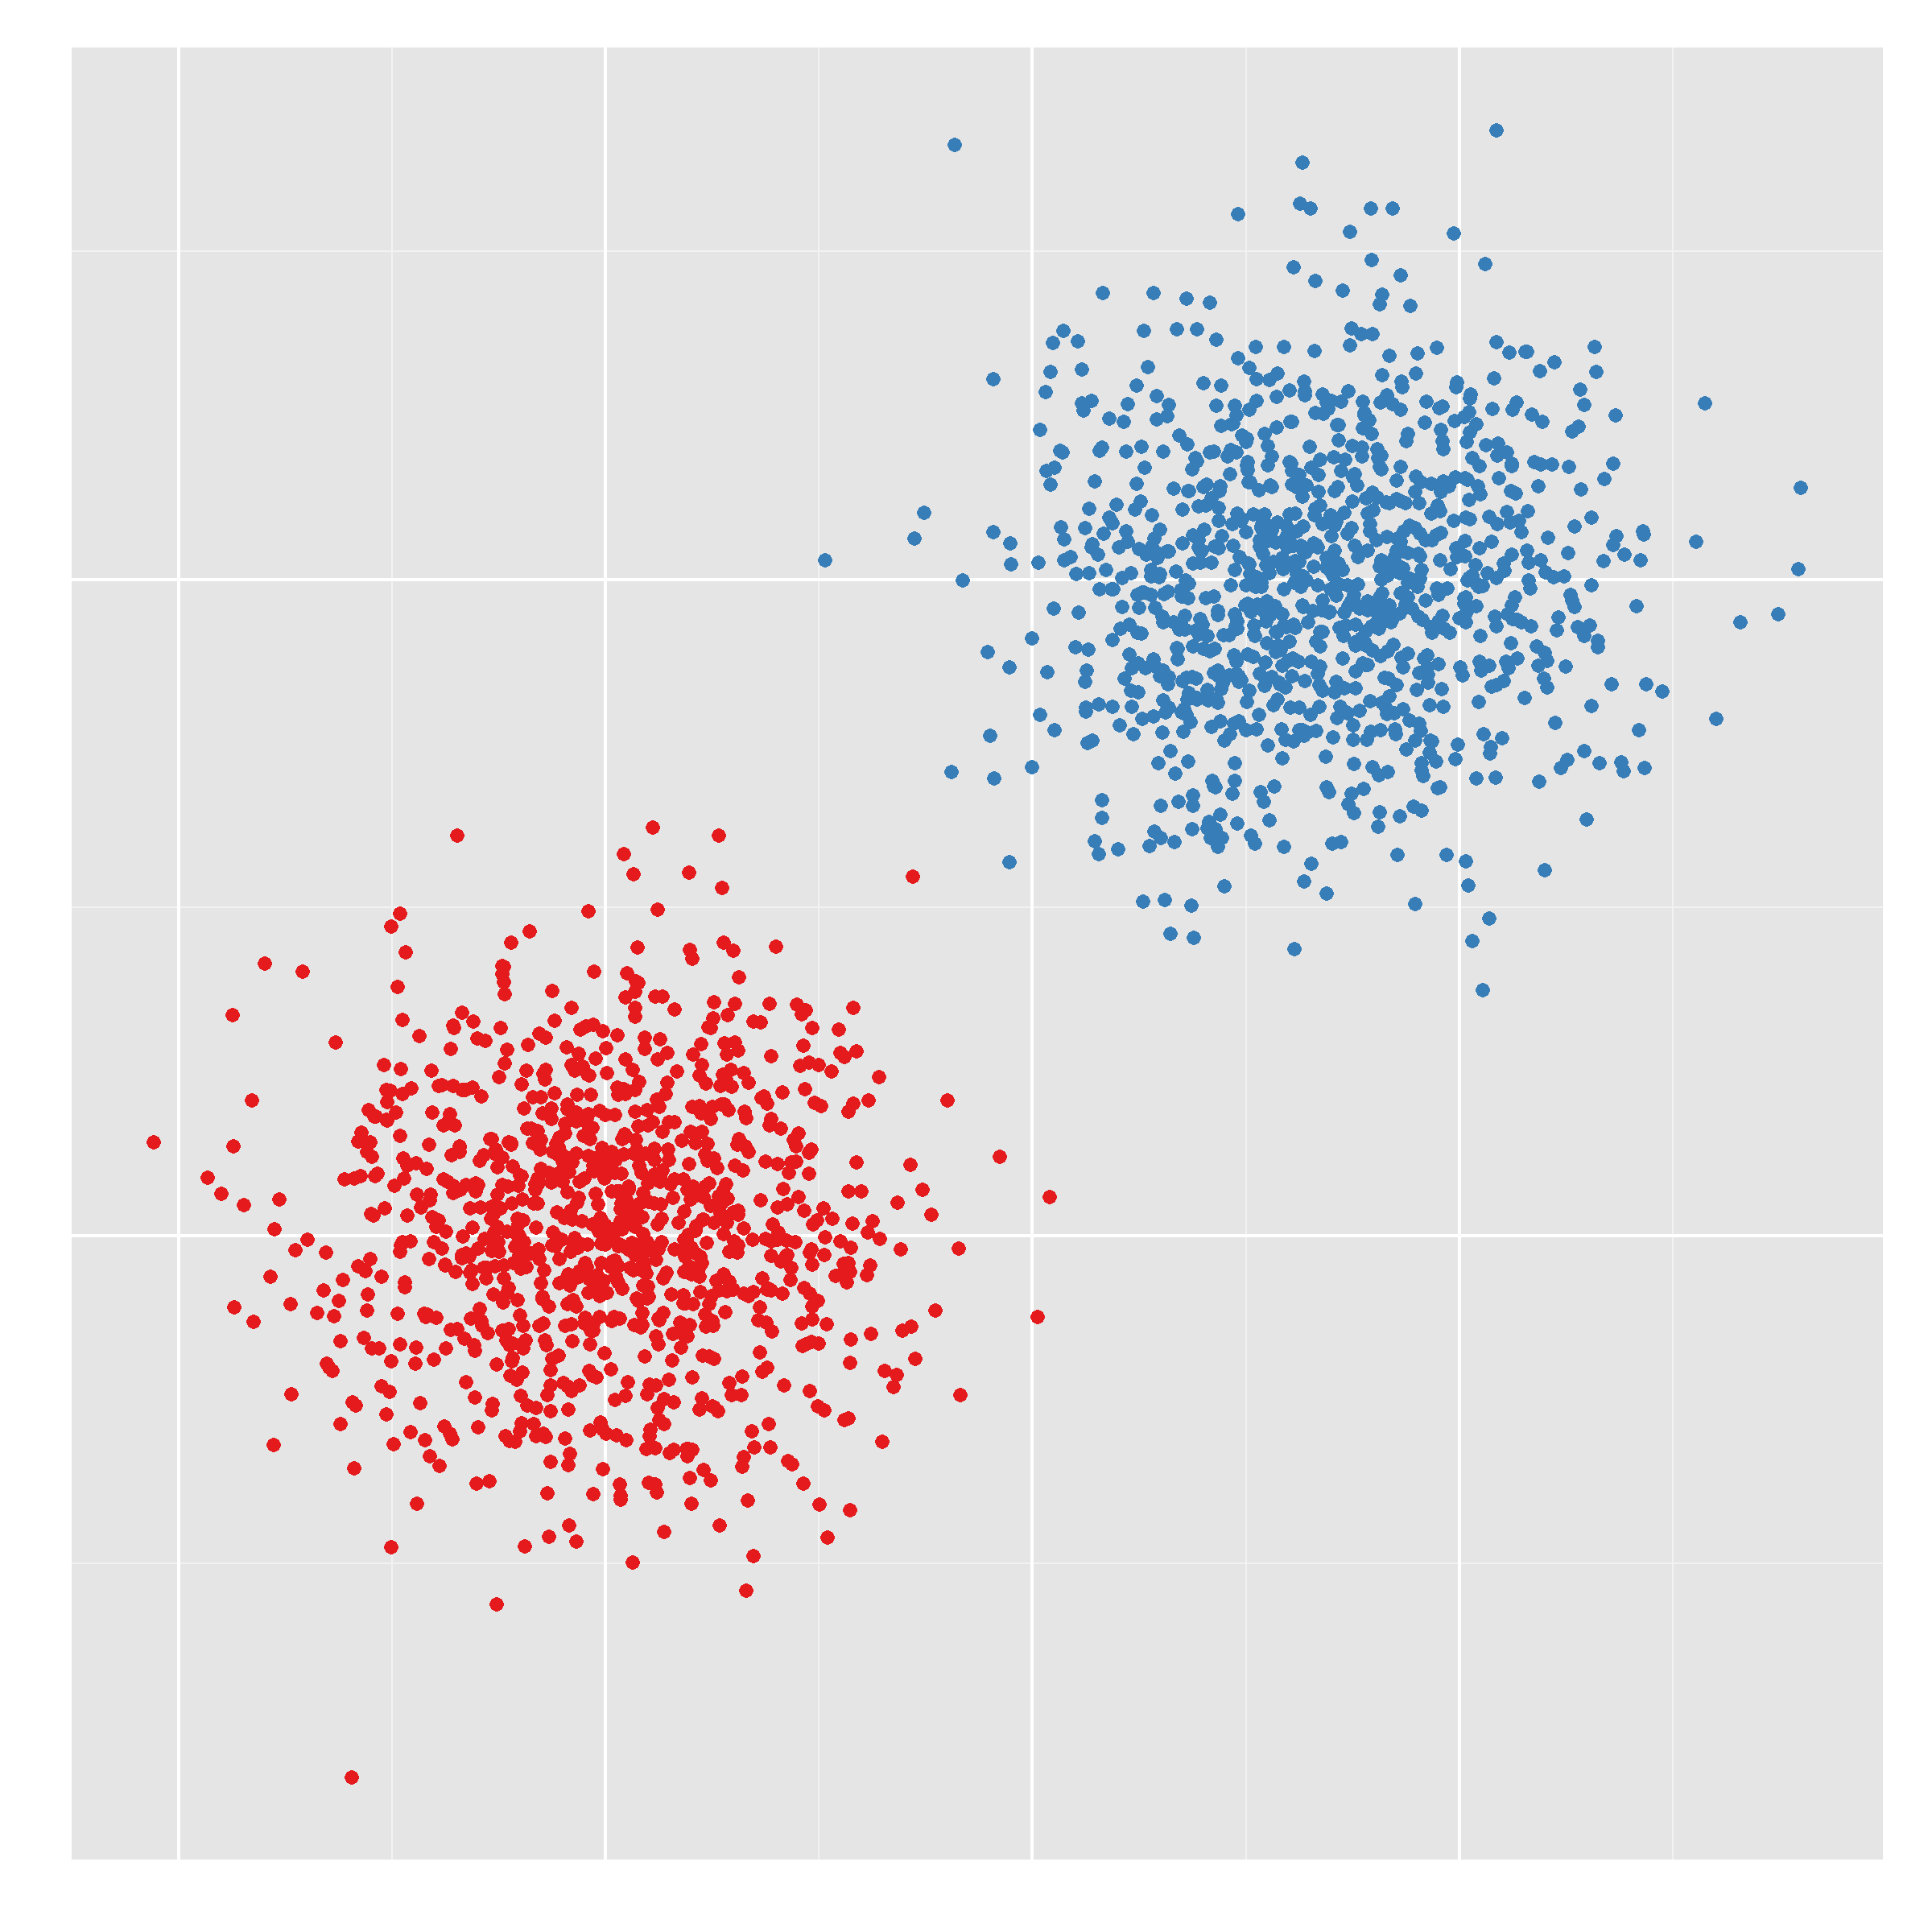
\includegraphics[width=.9\linewidth]{staticNormal}
  \caption{Static Normal}
  \label{fig:simdata1}
\end{subfigure}
\begin{subfigure}{.33\textwidth}
  \centering
  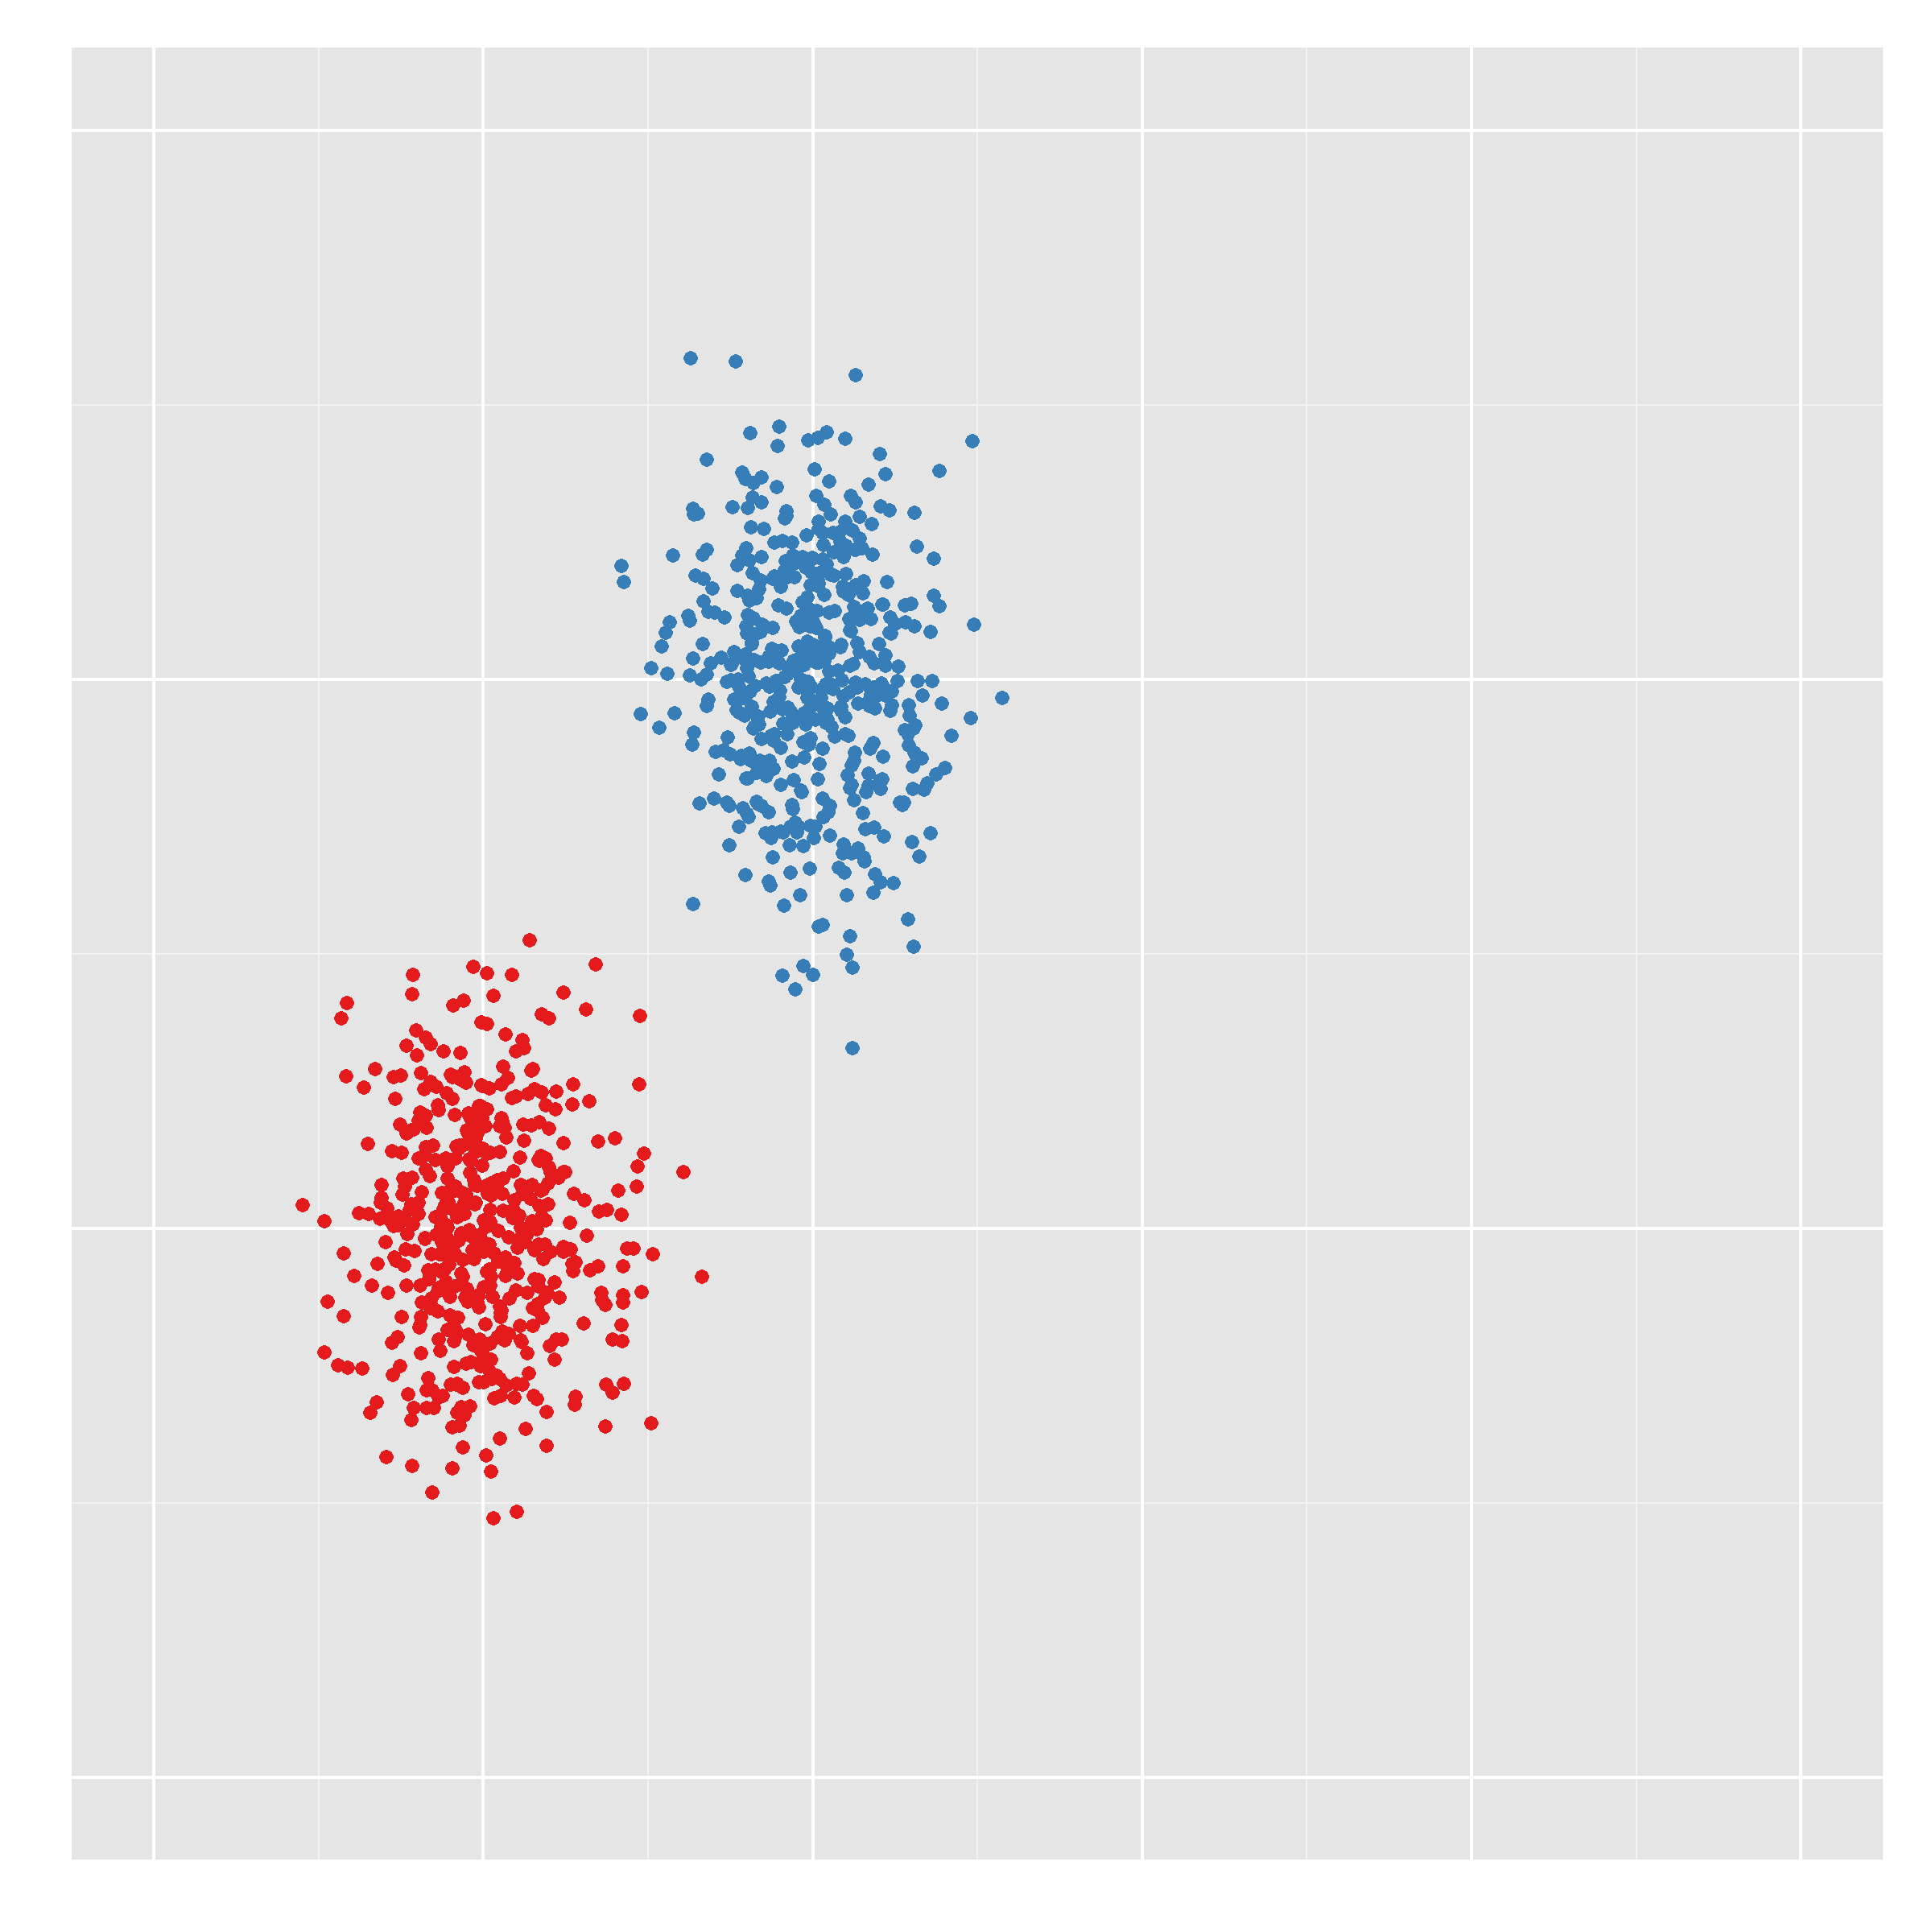
\includegraphics[width=.9\linewidth]{jumpNormal1.png}
  \caption{Jump start}
 \label{fig:simdata2}
\end{subfigure}%
\begin{subfigure}{.33\textwidth}
  \centering
  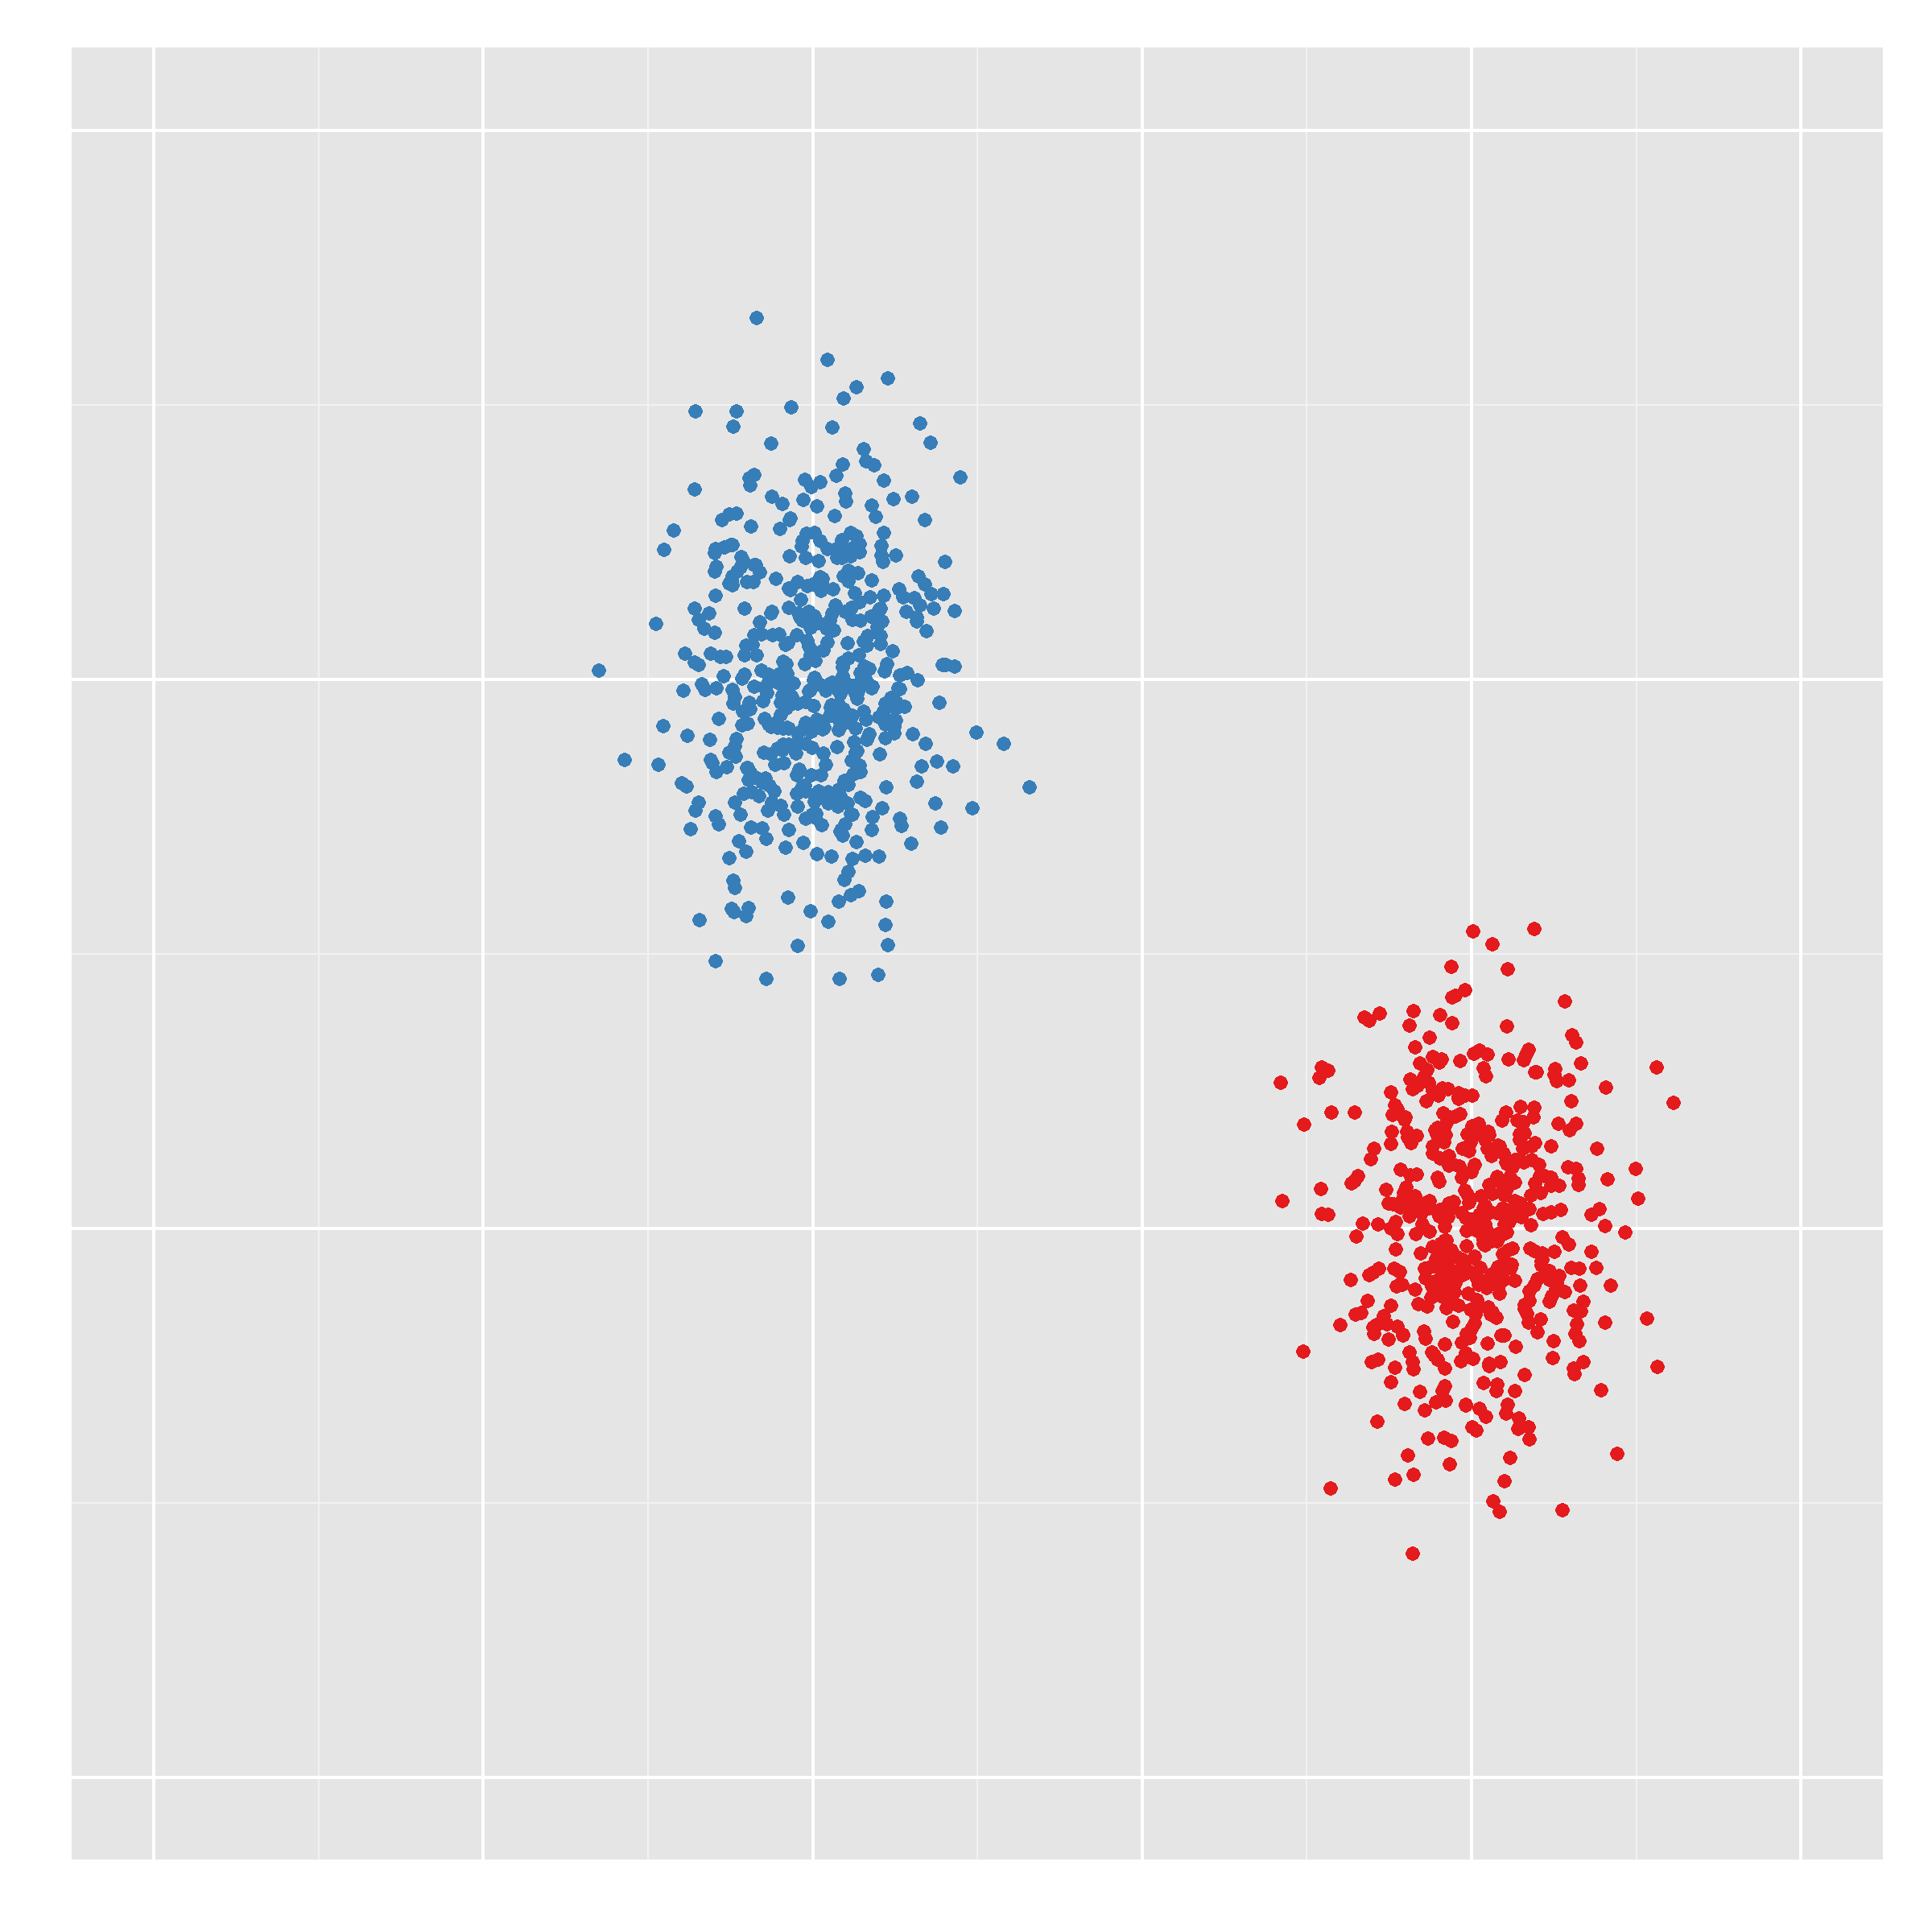
\includegraphics[width=.9\linewidth]{jumpNormal2.png}
  \caption{Jump End}
  \label{fig:simdata3}
\end{subfigure}
\begin{subfigure}{.33\textwidth}
  \centering
  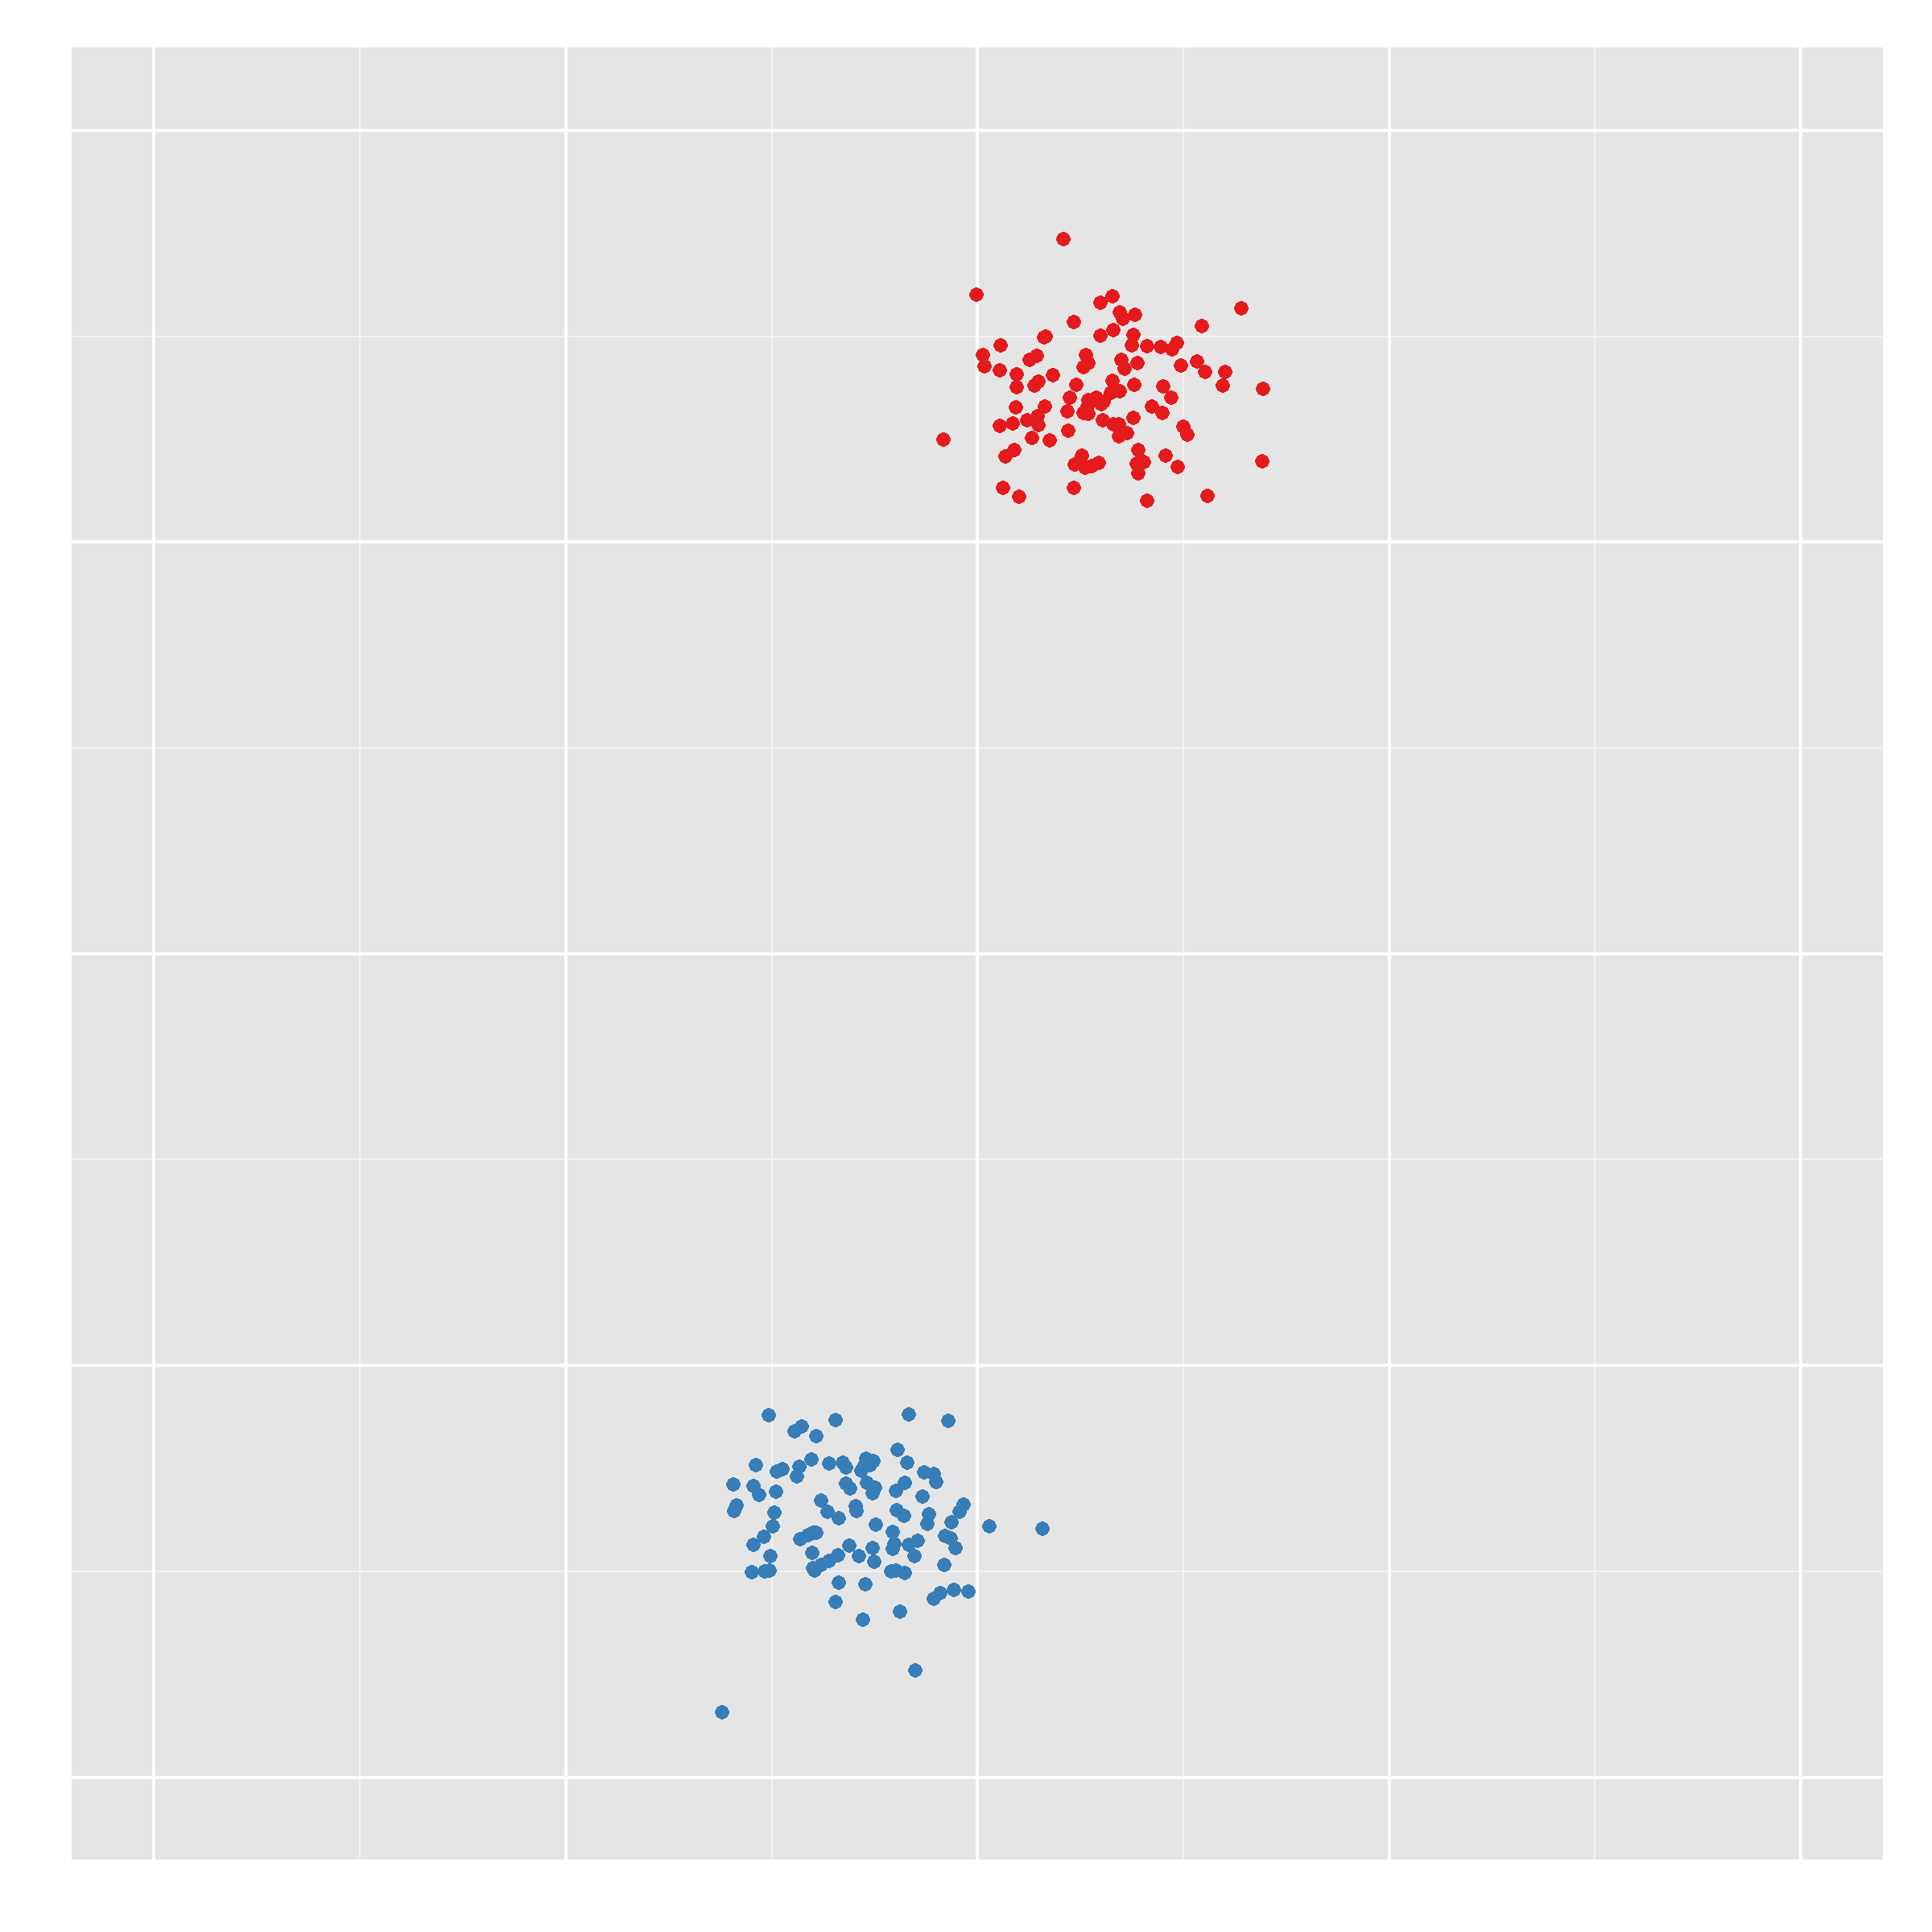
\includegraphics[width=.9\linewidth]{hyperSphere500_700.png}
  \caption{Evolving Start}
 \label{fig:simdata4}
\end{subfigure}%
\begin{subfigure}{.33\textwidth}
  \centering
  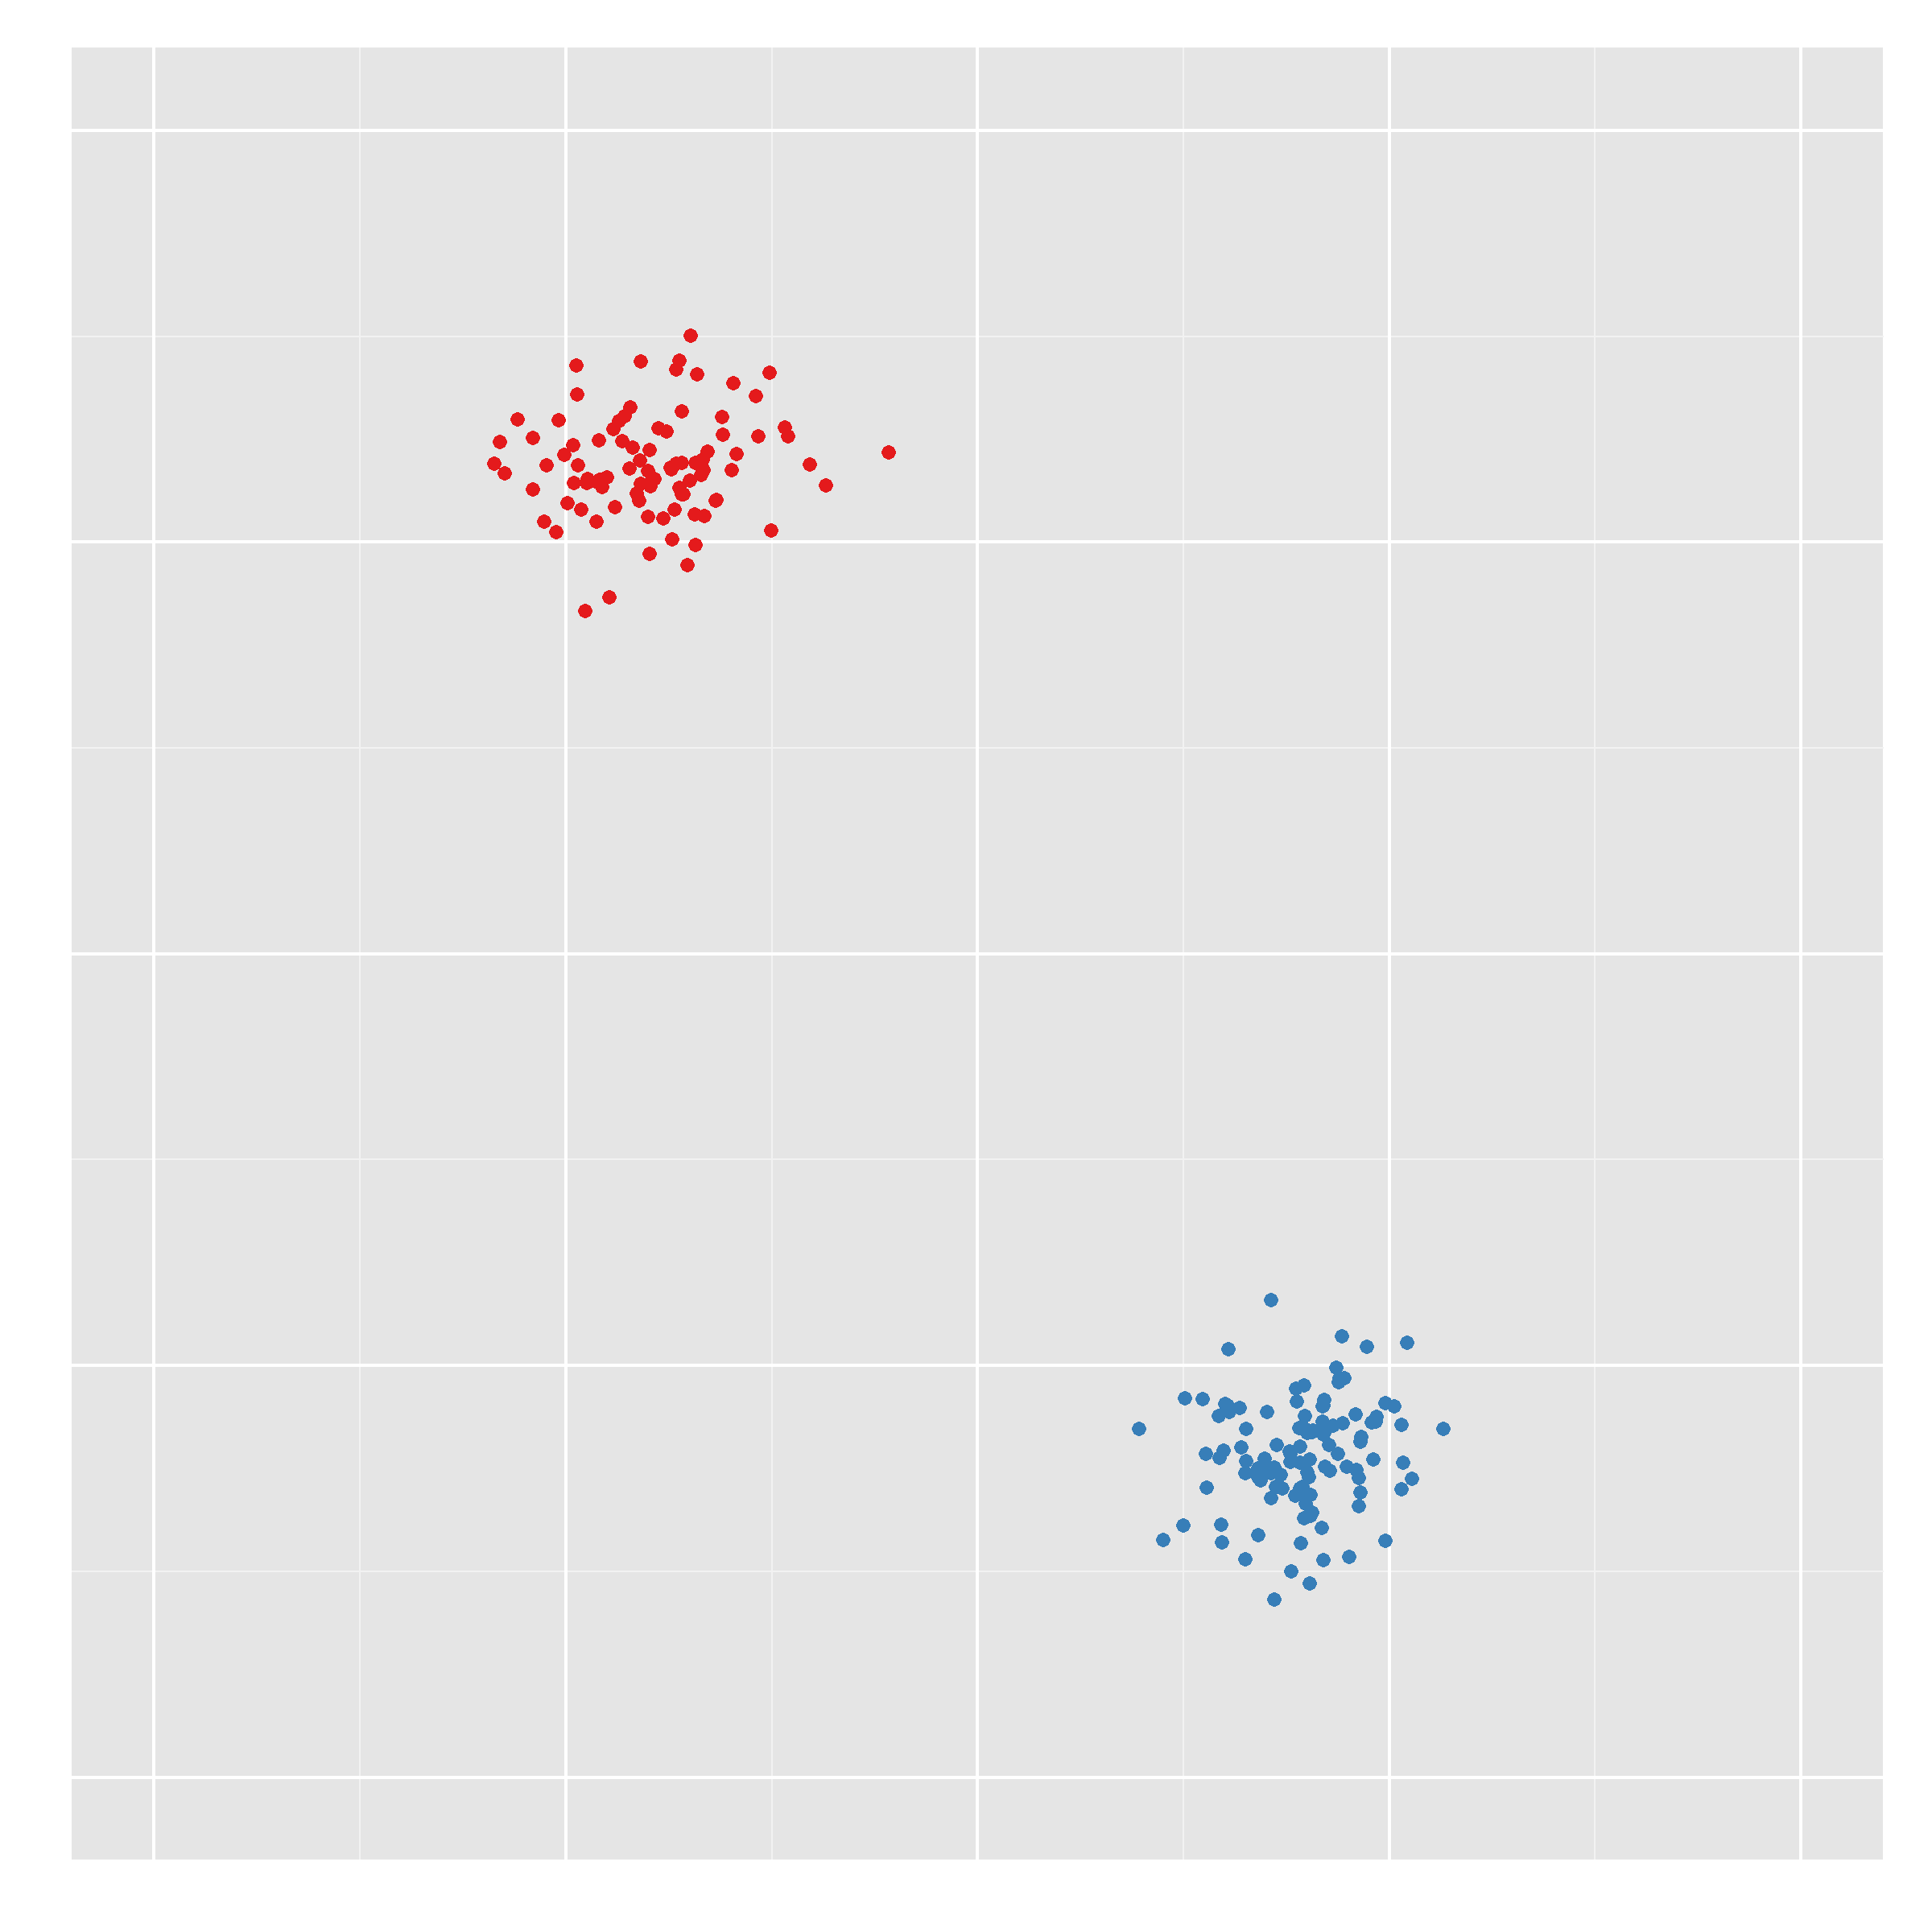
\includegraphics[width=.9\linewidth]{hyperSphere1200_1400.png}
  \caption{Evolving Middle}
  \label{fig:simdata5}
\end{subfigure}
\begin{subfigure}{.33\textwidth}
  \centering
  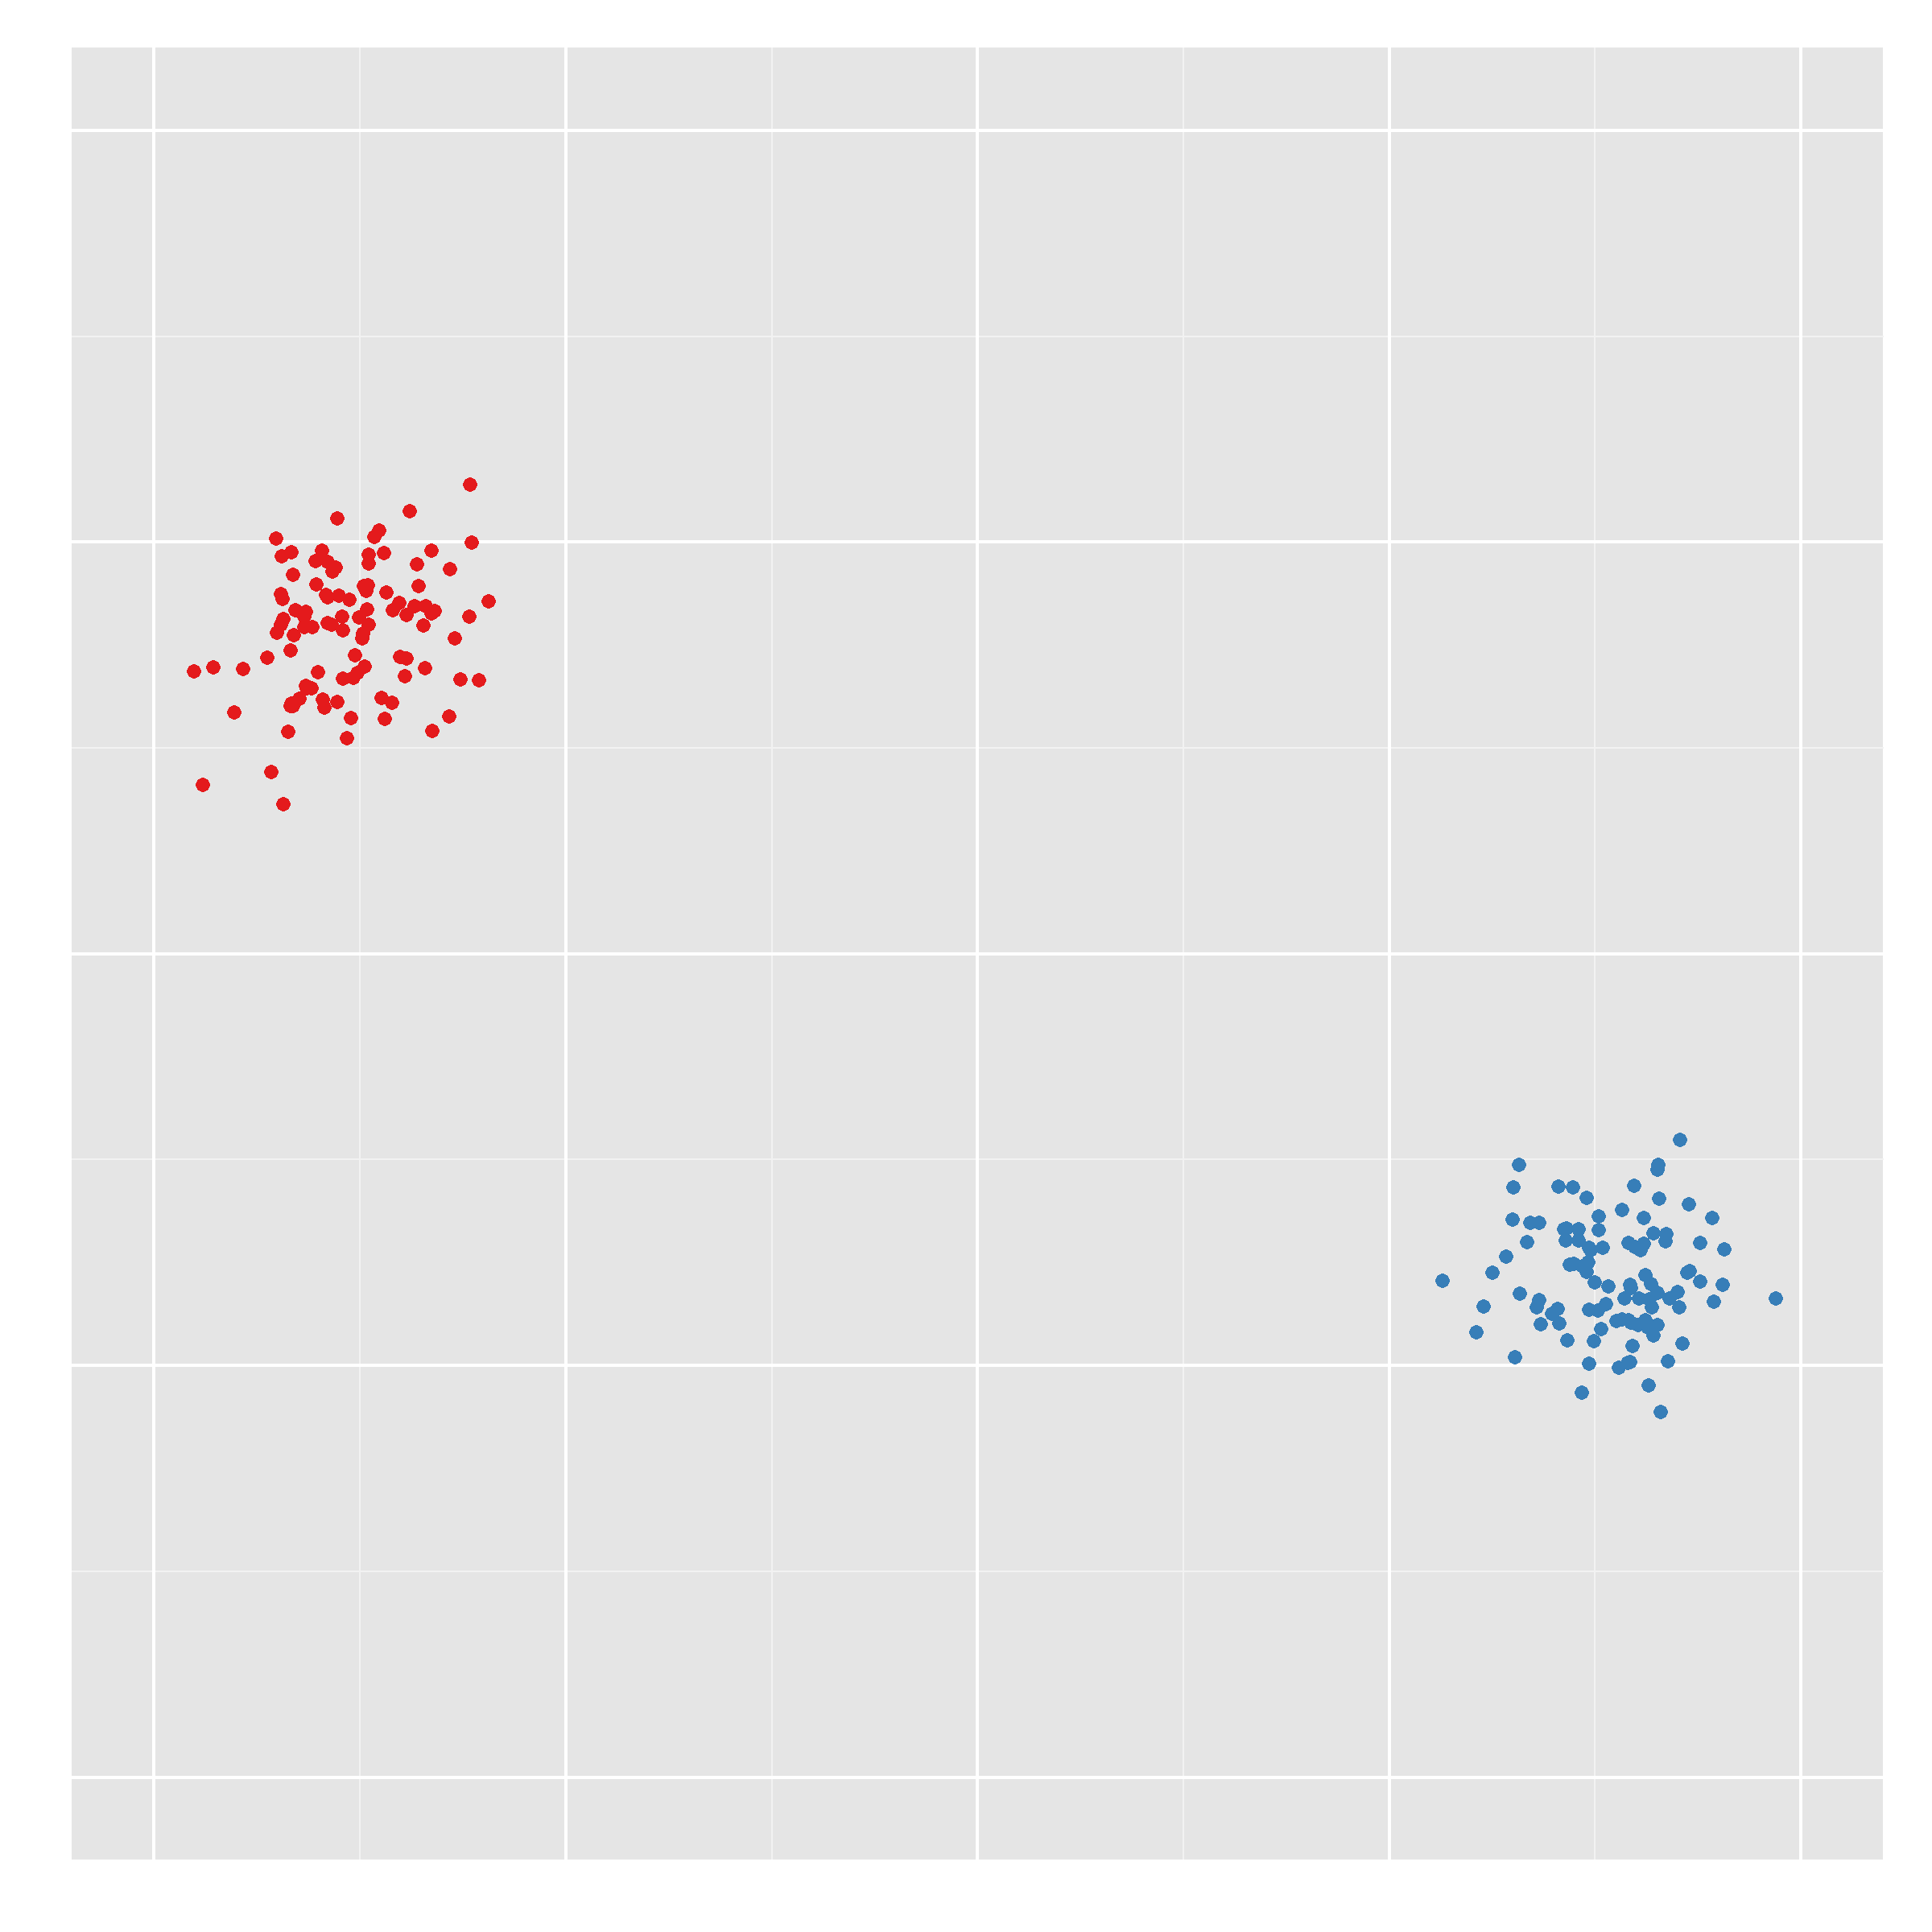
\includegraphics[width=.9\linewidth]{hyperSphere1800_2000.png}
  \caption{Evolving End}
 \label{fig:simdata6}
\end{subfigure}%
\caption{Descriptions of the simulated data sets. Figure \ref{fig:simdata1} shows the Static Normal Data set. Figures (\ref{fig:simdata2}, \ref{fig:simdata3}) shows the Jump data set before and after the changepoint. Figures (\ref{fig:simdata4}, \ref{fig:simdata5},\ref{fig:simdata6}) show the evolving data set at the start, in the middle and at the end of the stream.  }
\label{fig:simulated_clustream}
\end{figure}

 Figure \ref{fig:simulated_clustream} shows performance of unweighted spectral clustream, weighted spectral clustream and windowed spectral clustering on a number of simulated data sets. 

\begin{figure}[h!]
\begin{subfigure}{.5\textwidth}
  \centering
  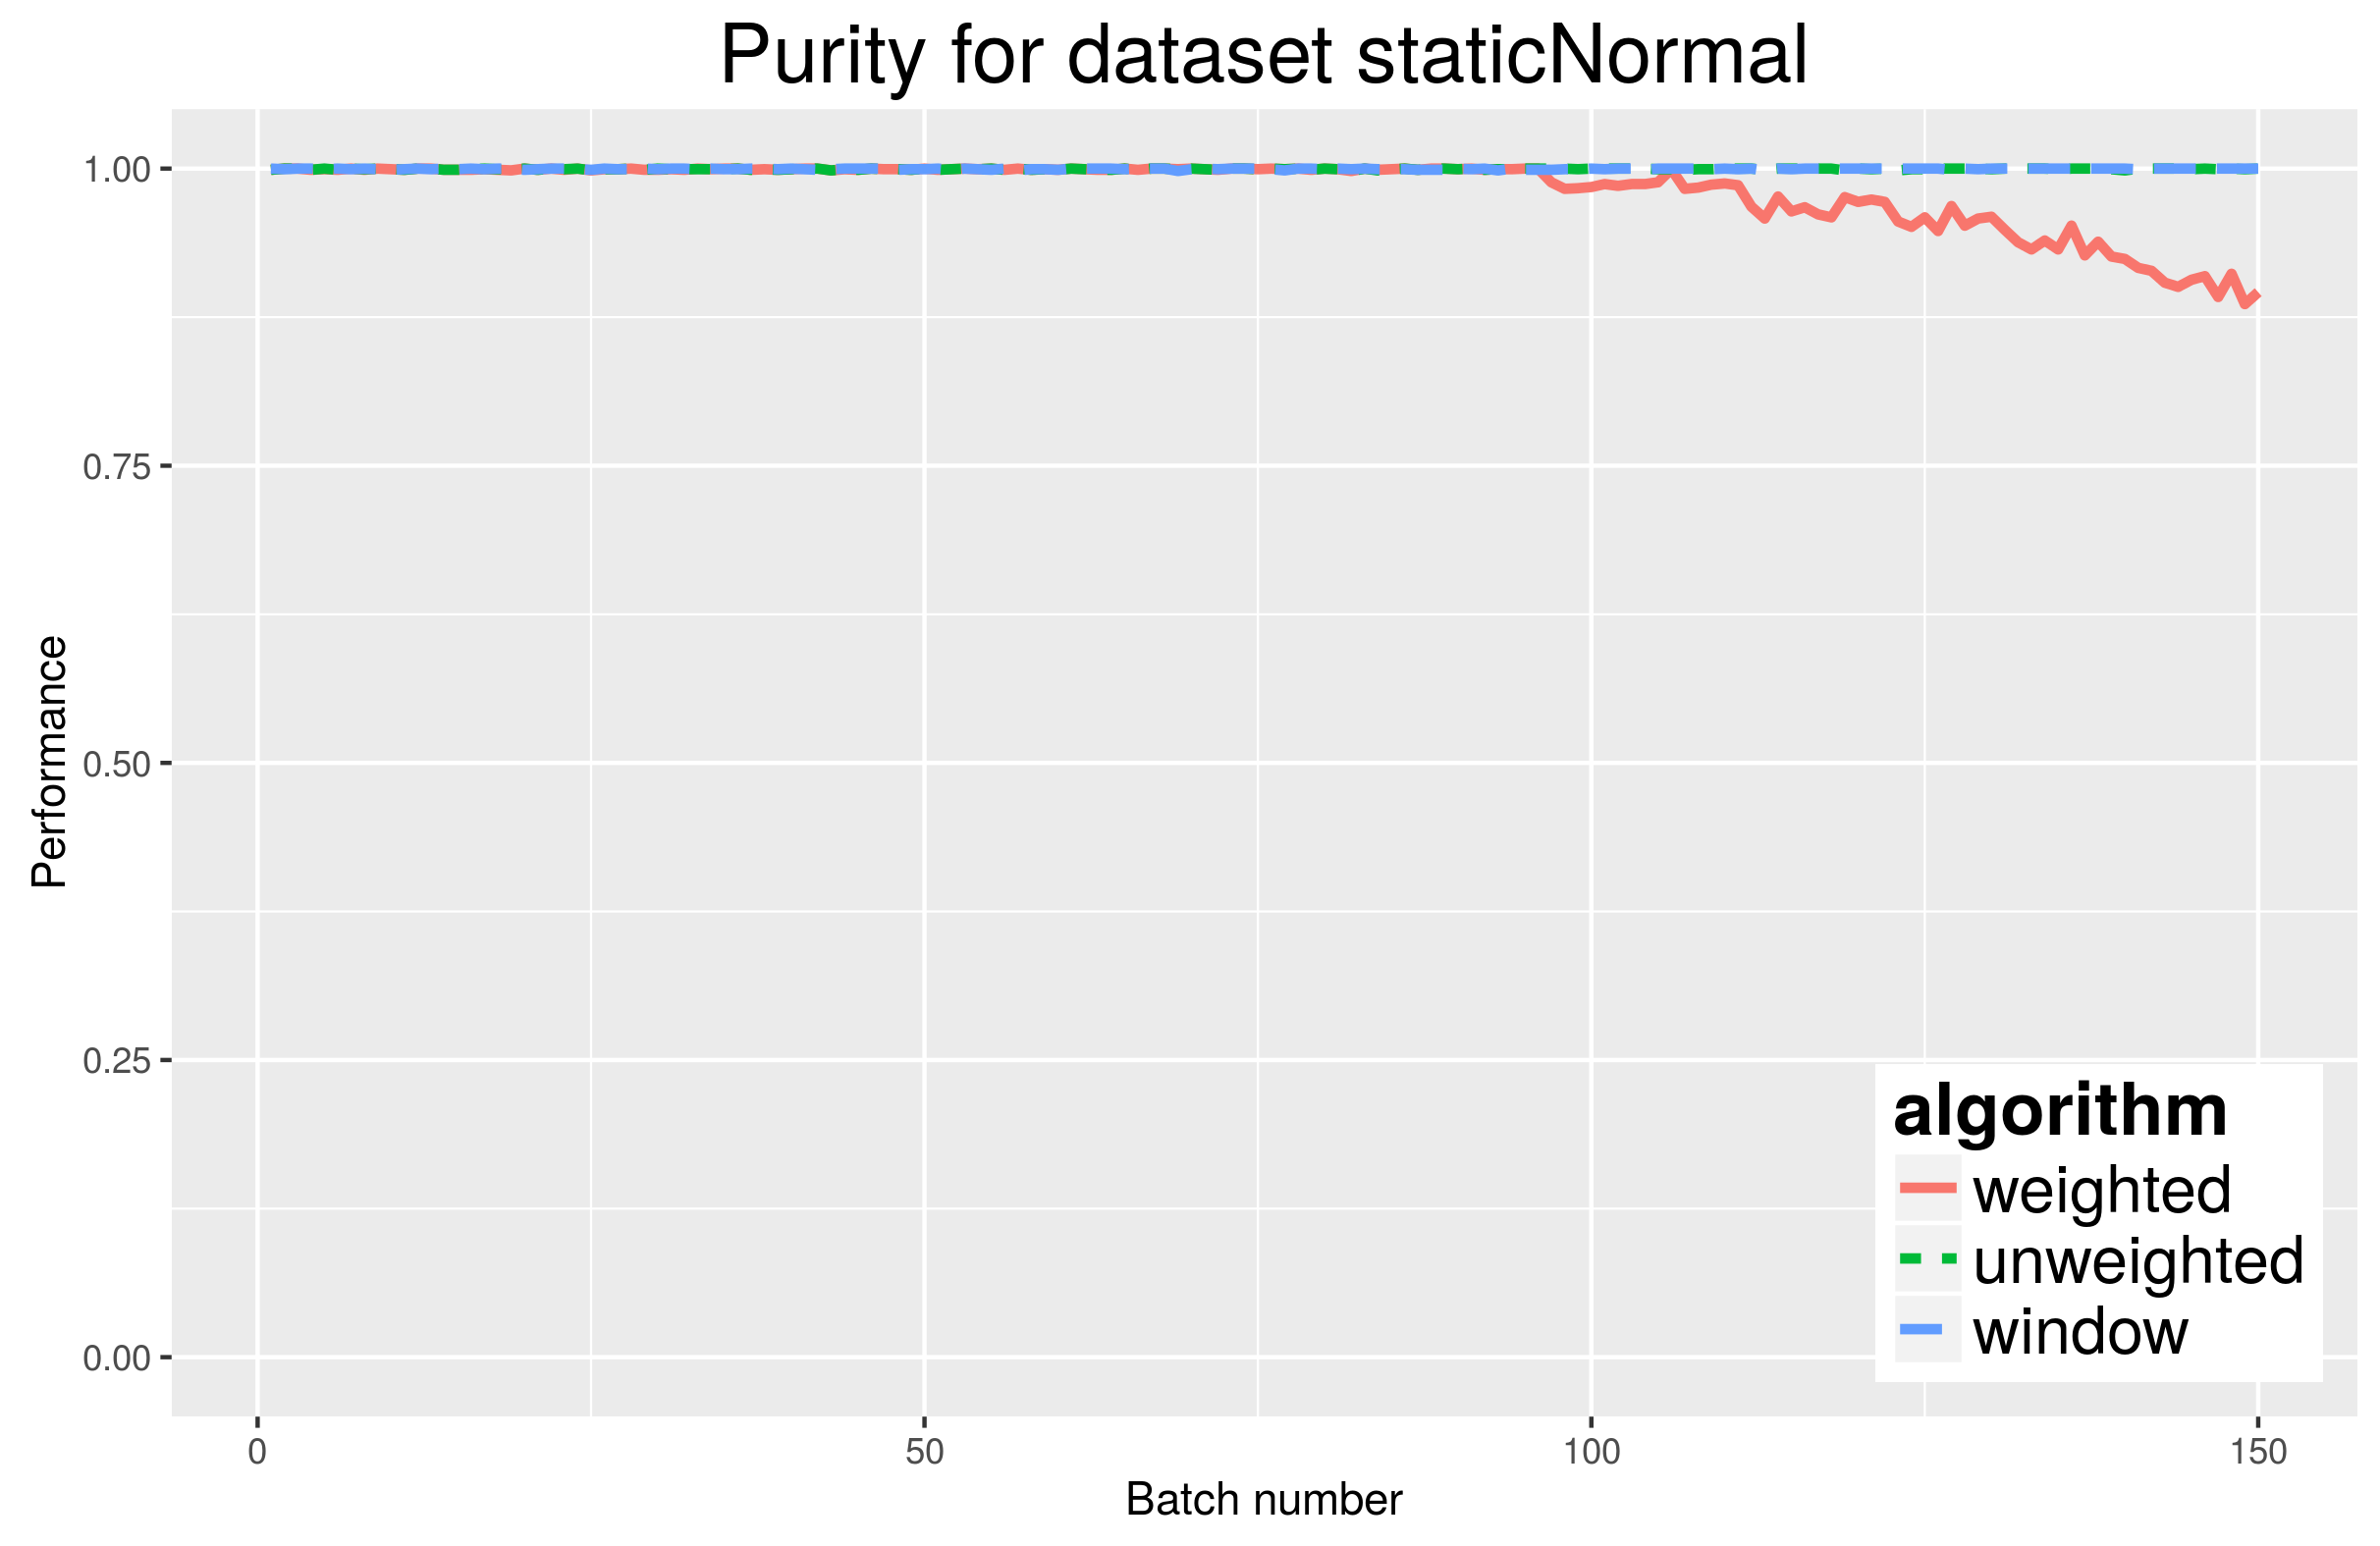
\includegraphics[width=.9\linewidth]{staticNormal_purity}
  \caption{Static Normal Purity}
 % \label{fig:sfig1}
\end{subfigure}%
\begin{subfigure}{.5\textwidth}
  \centering
  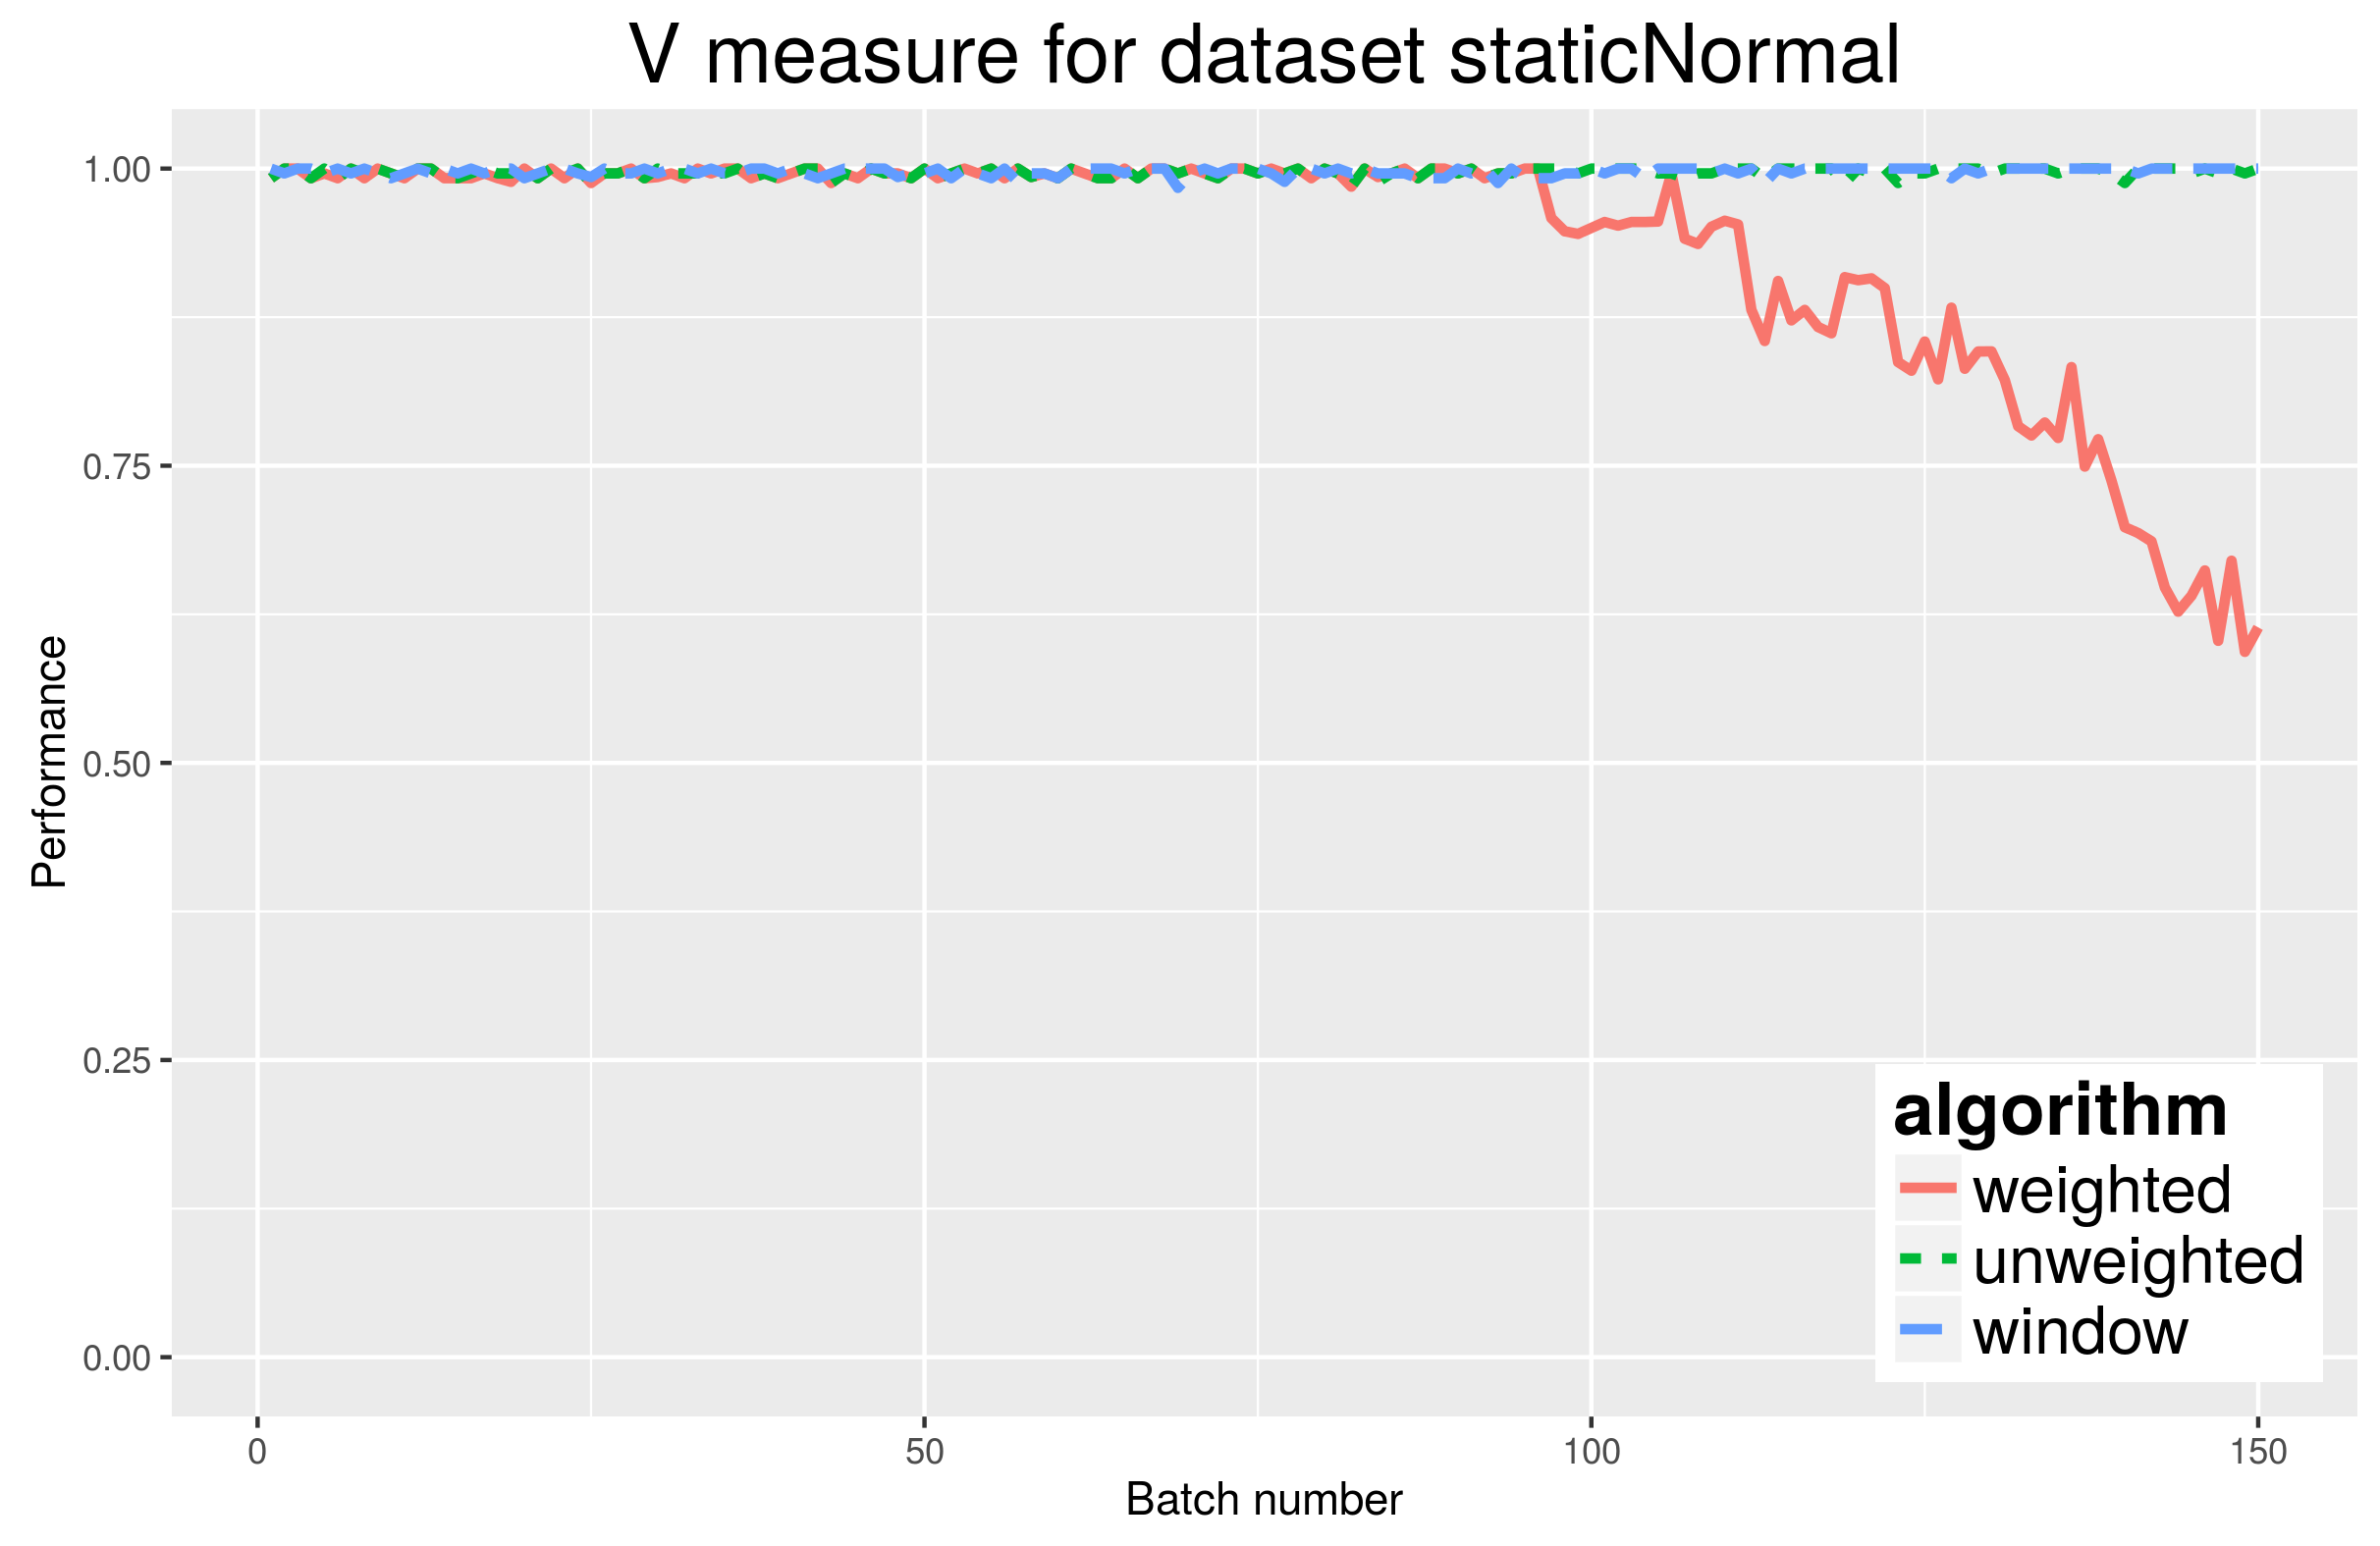
\includegraphics[width=.9\linewidth]{staticNormal_vmeasure}
  \caption{Static Normal V-measure}
%  \label{fig:sfig2}
\end{subfigure}
\begin{subfigure}{.5\textwidth}
  \centering
  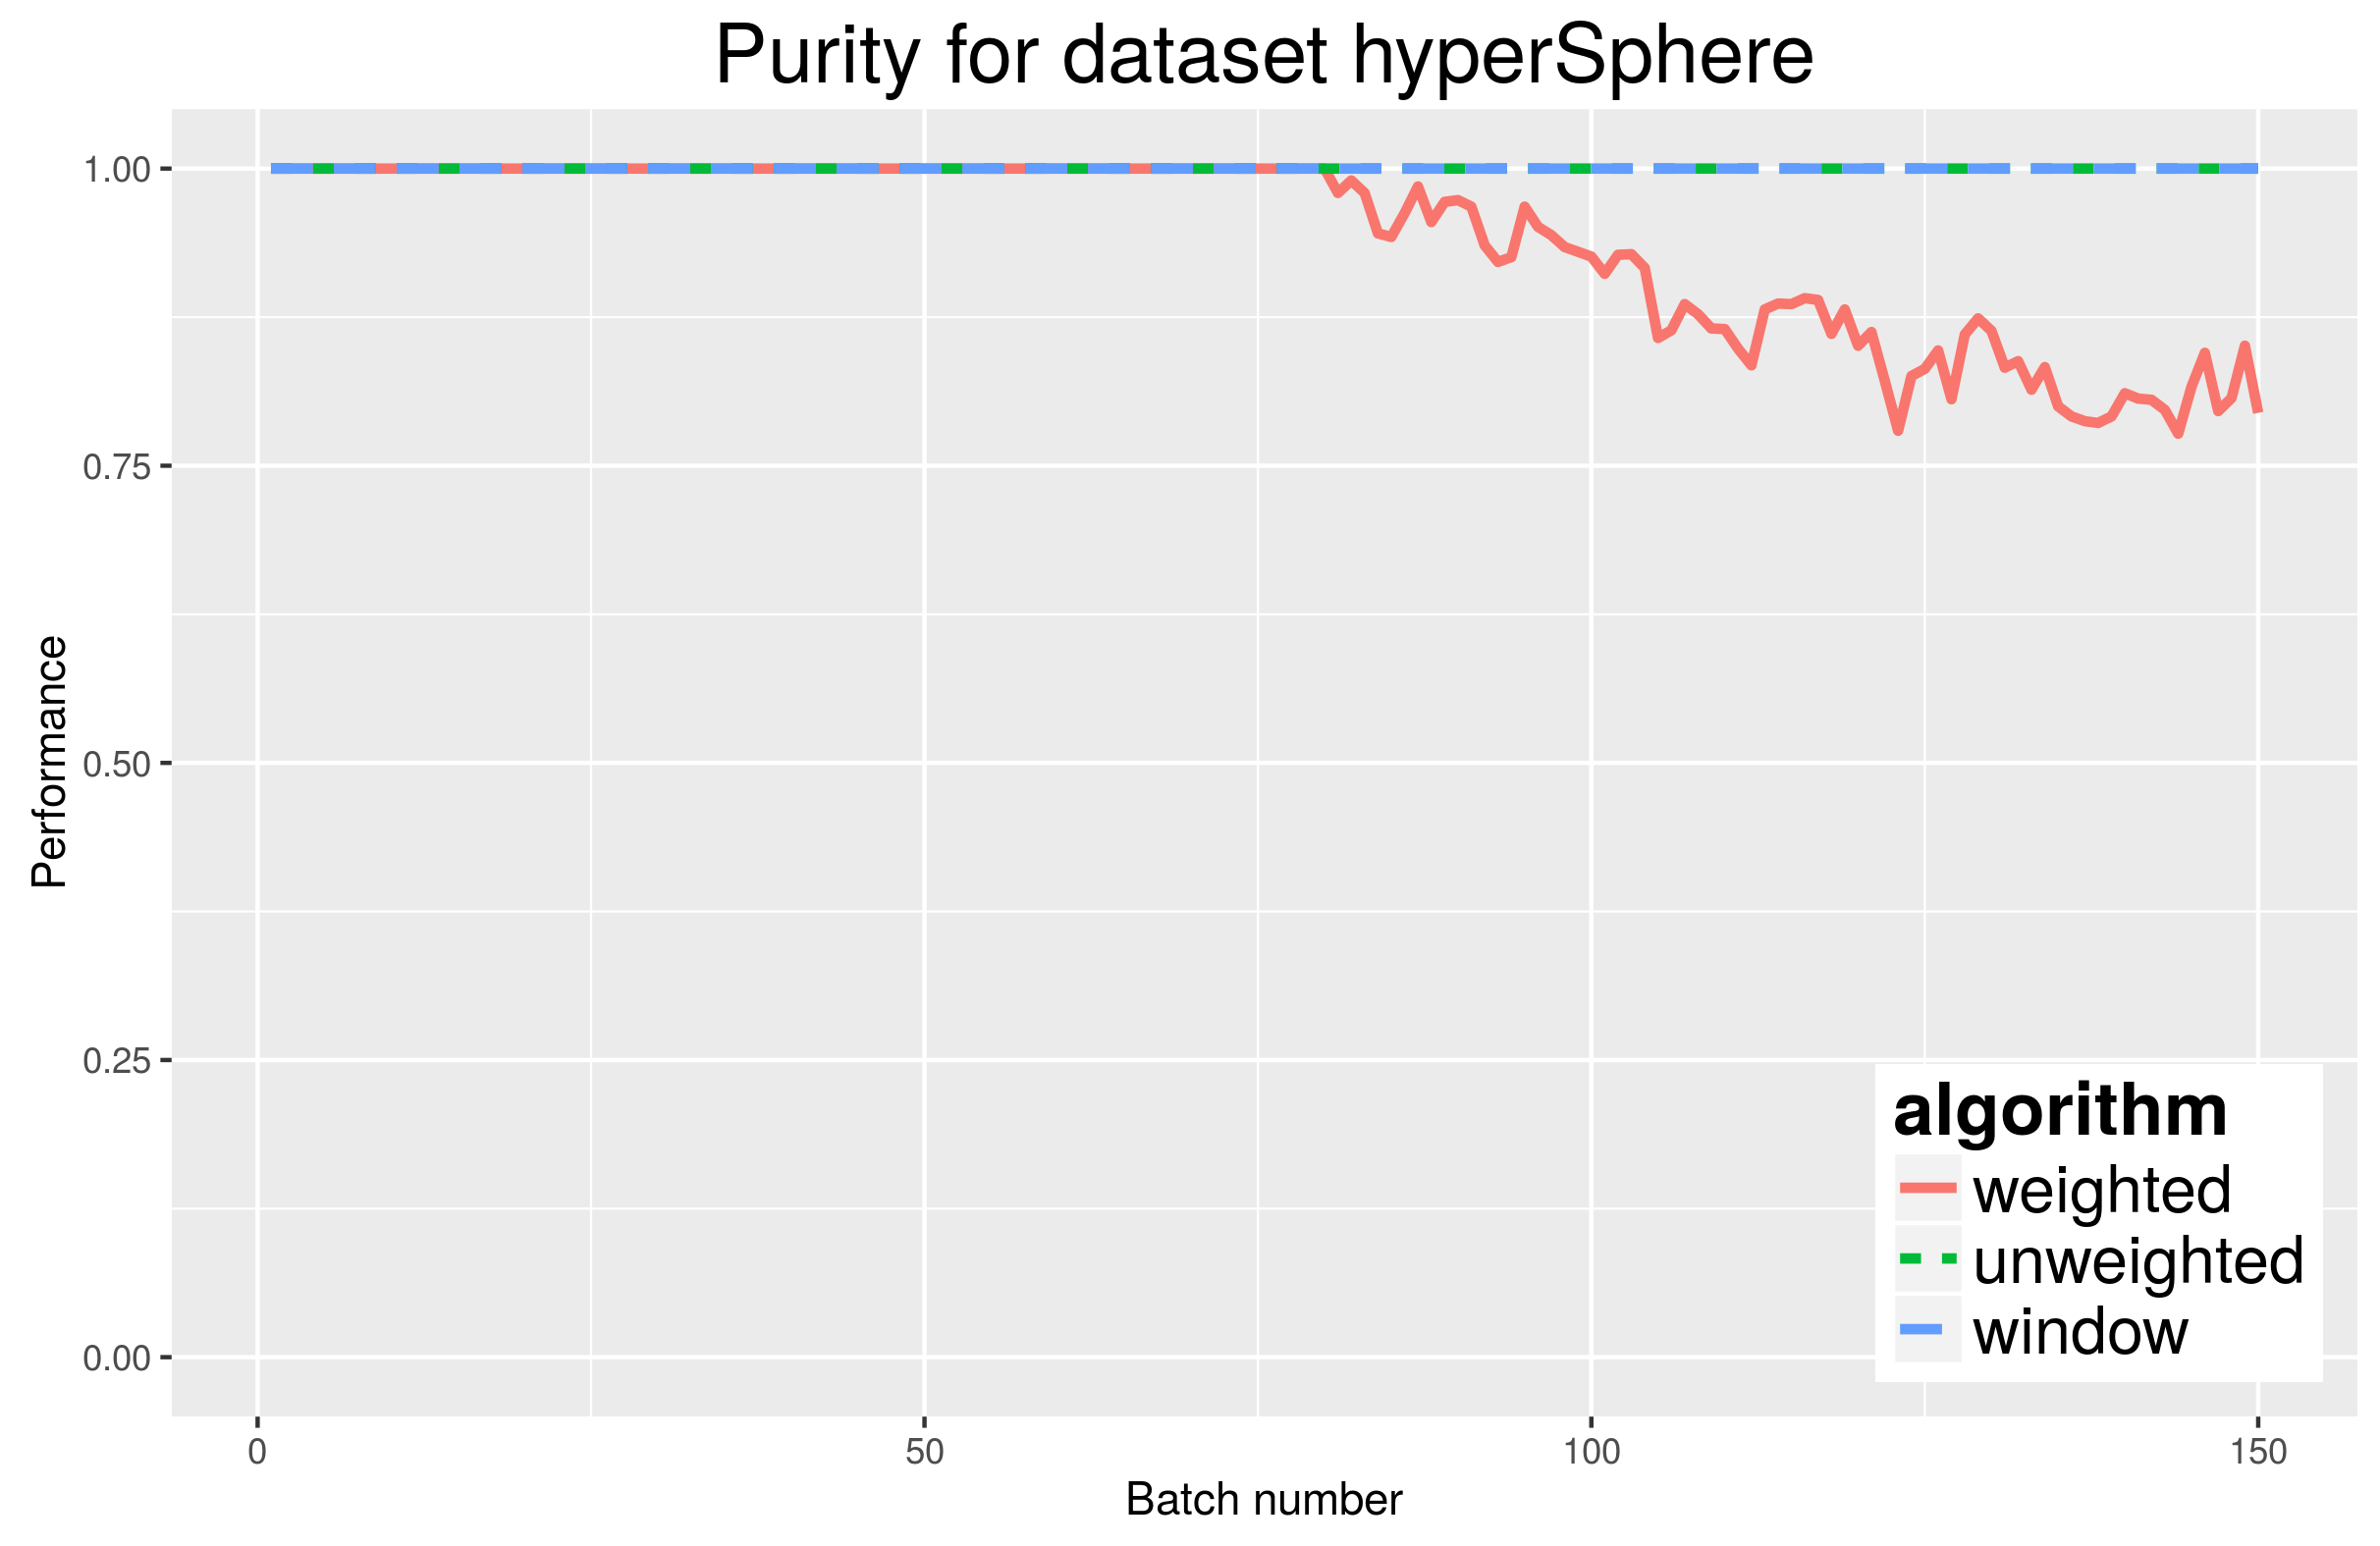
\includegraphics[width=.9\linewidth]{hyperSphere_purity}
  \caption{Evolving Normal Purity}
 % \label{fig:sfig1}
\end{subfigure}%
\begin{subfigure}{.5\textwidth}
  \centering
  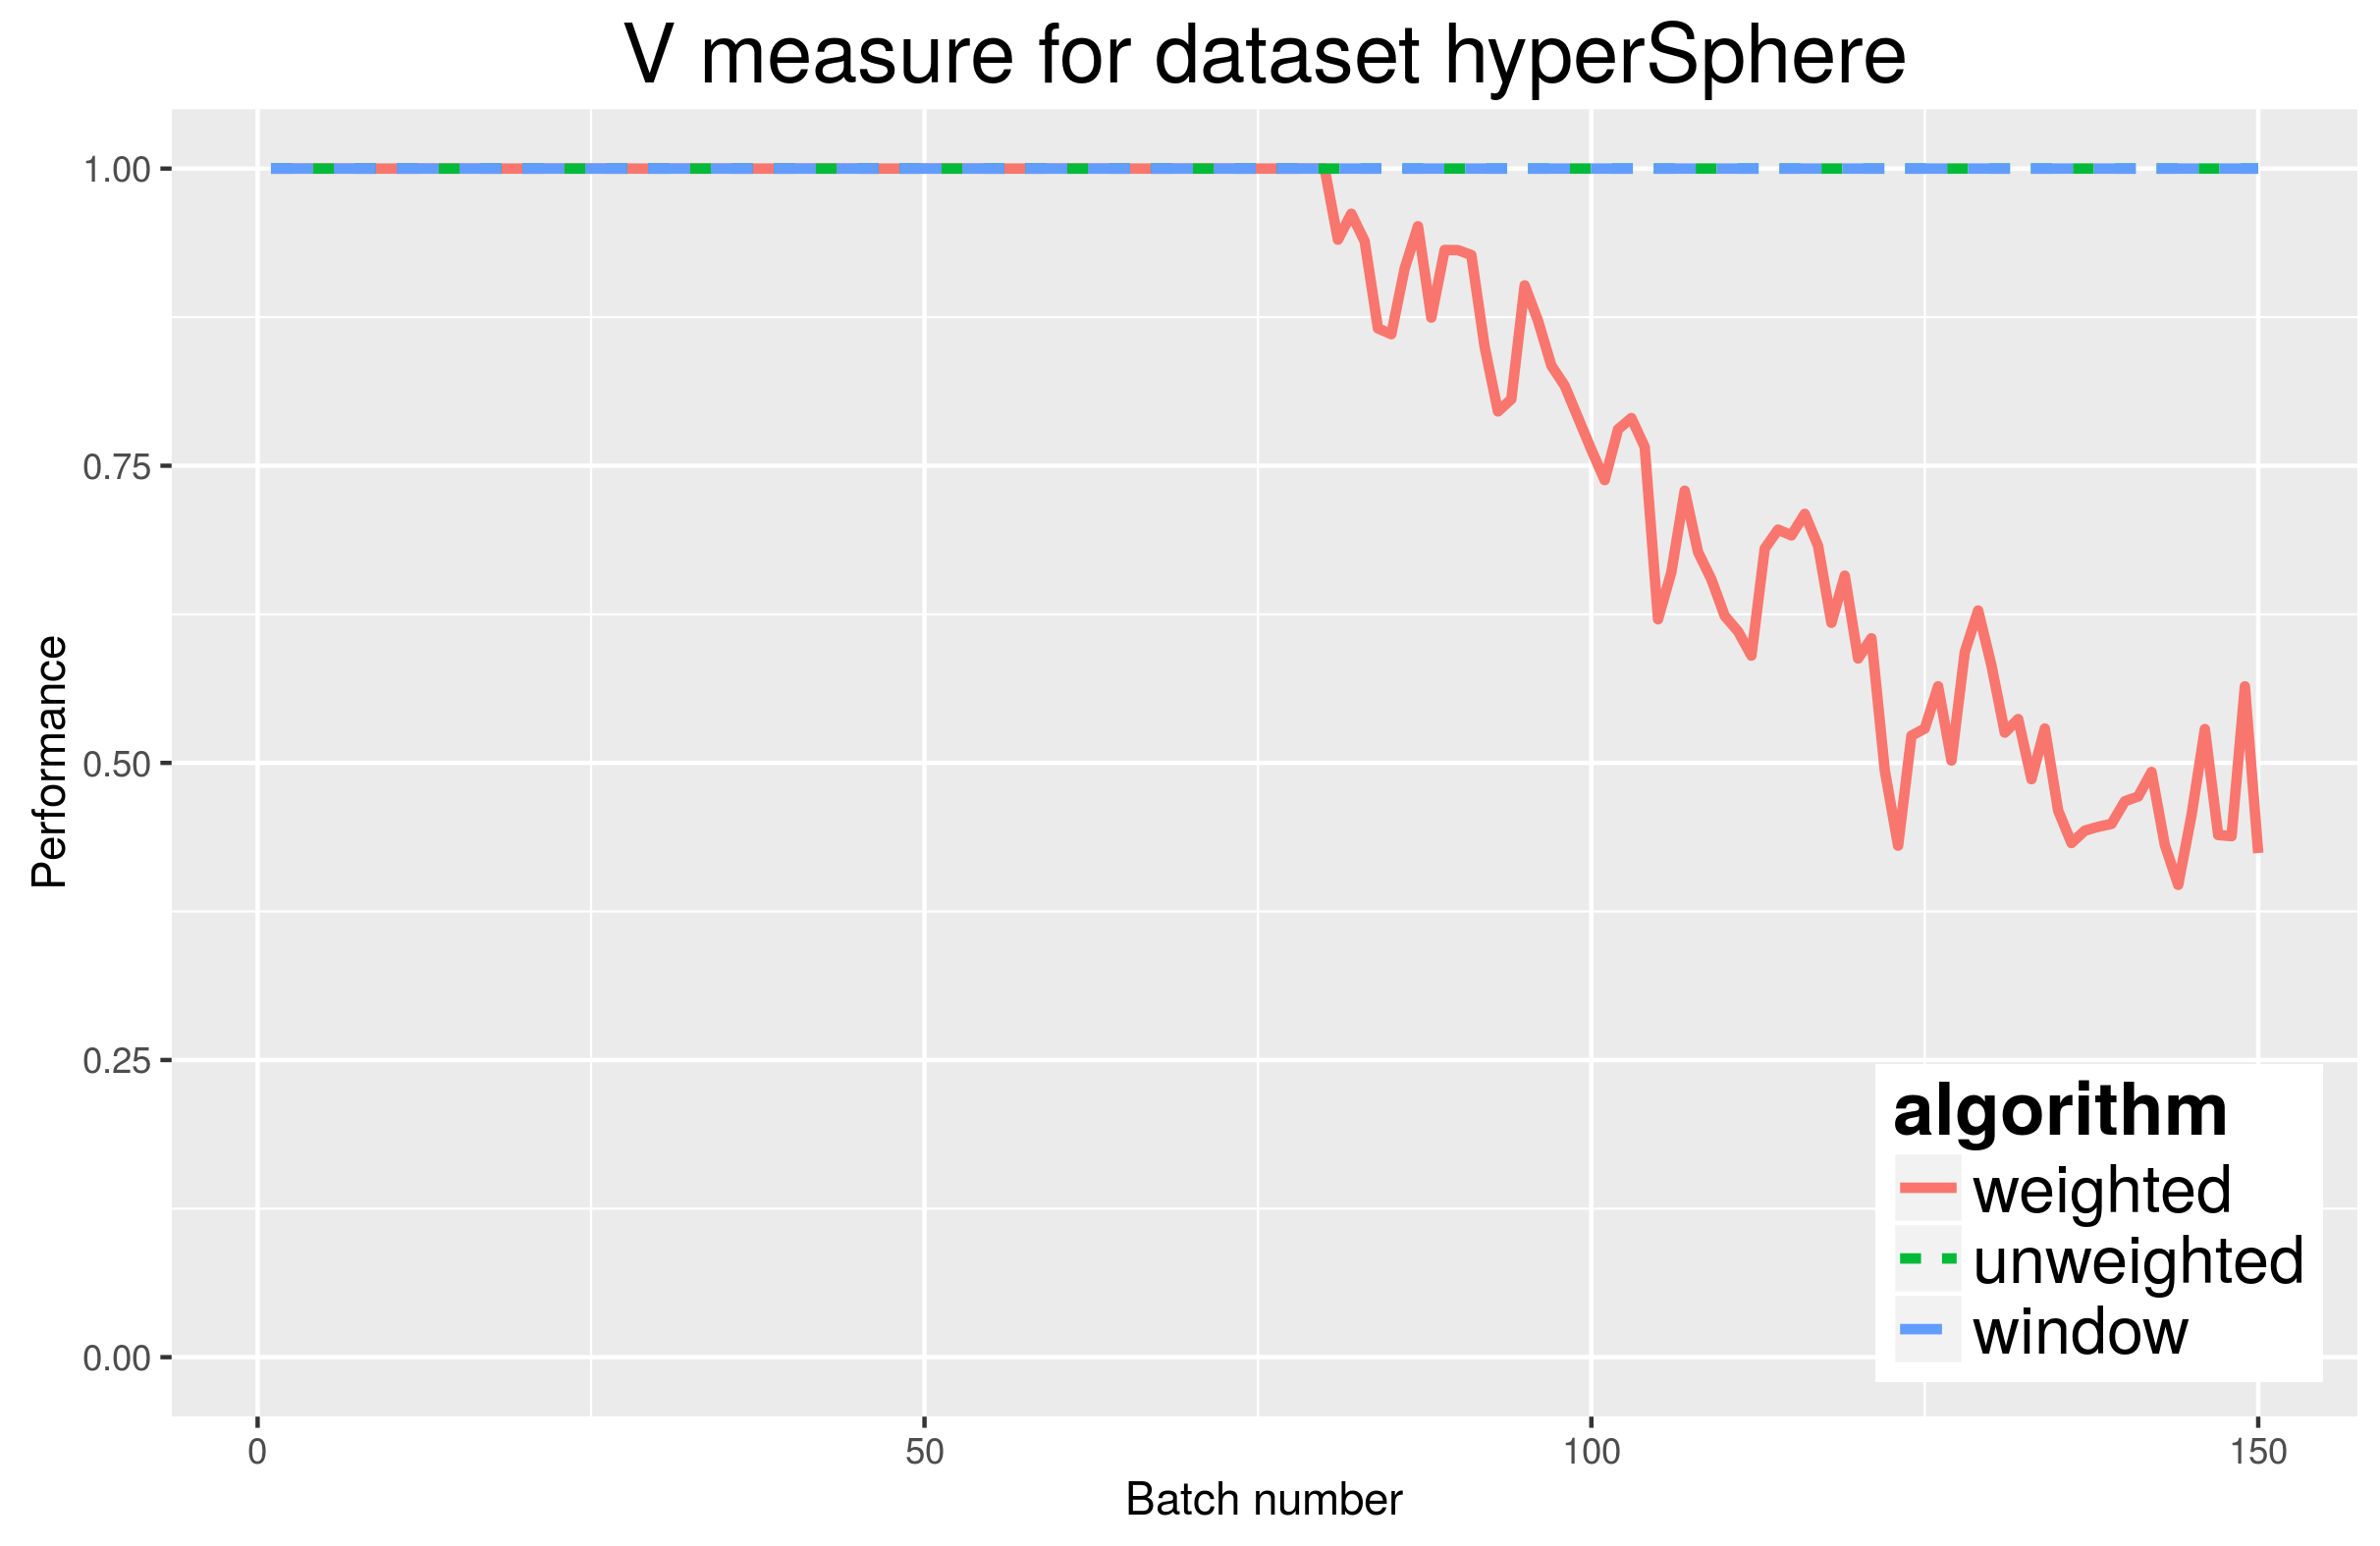
\includegraphics[width=.9\linewidth]{hyperSphere_vmeasure}
  \caption{Evolving Normal V-measure}
%  \label{fig:sfig2}
\end{subfigure}
\begin{subfigure}{.5\textwidth}
  \centering
  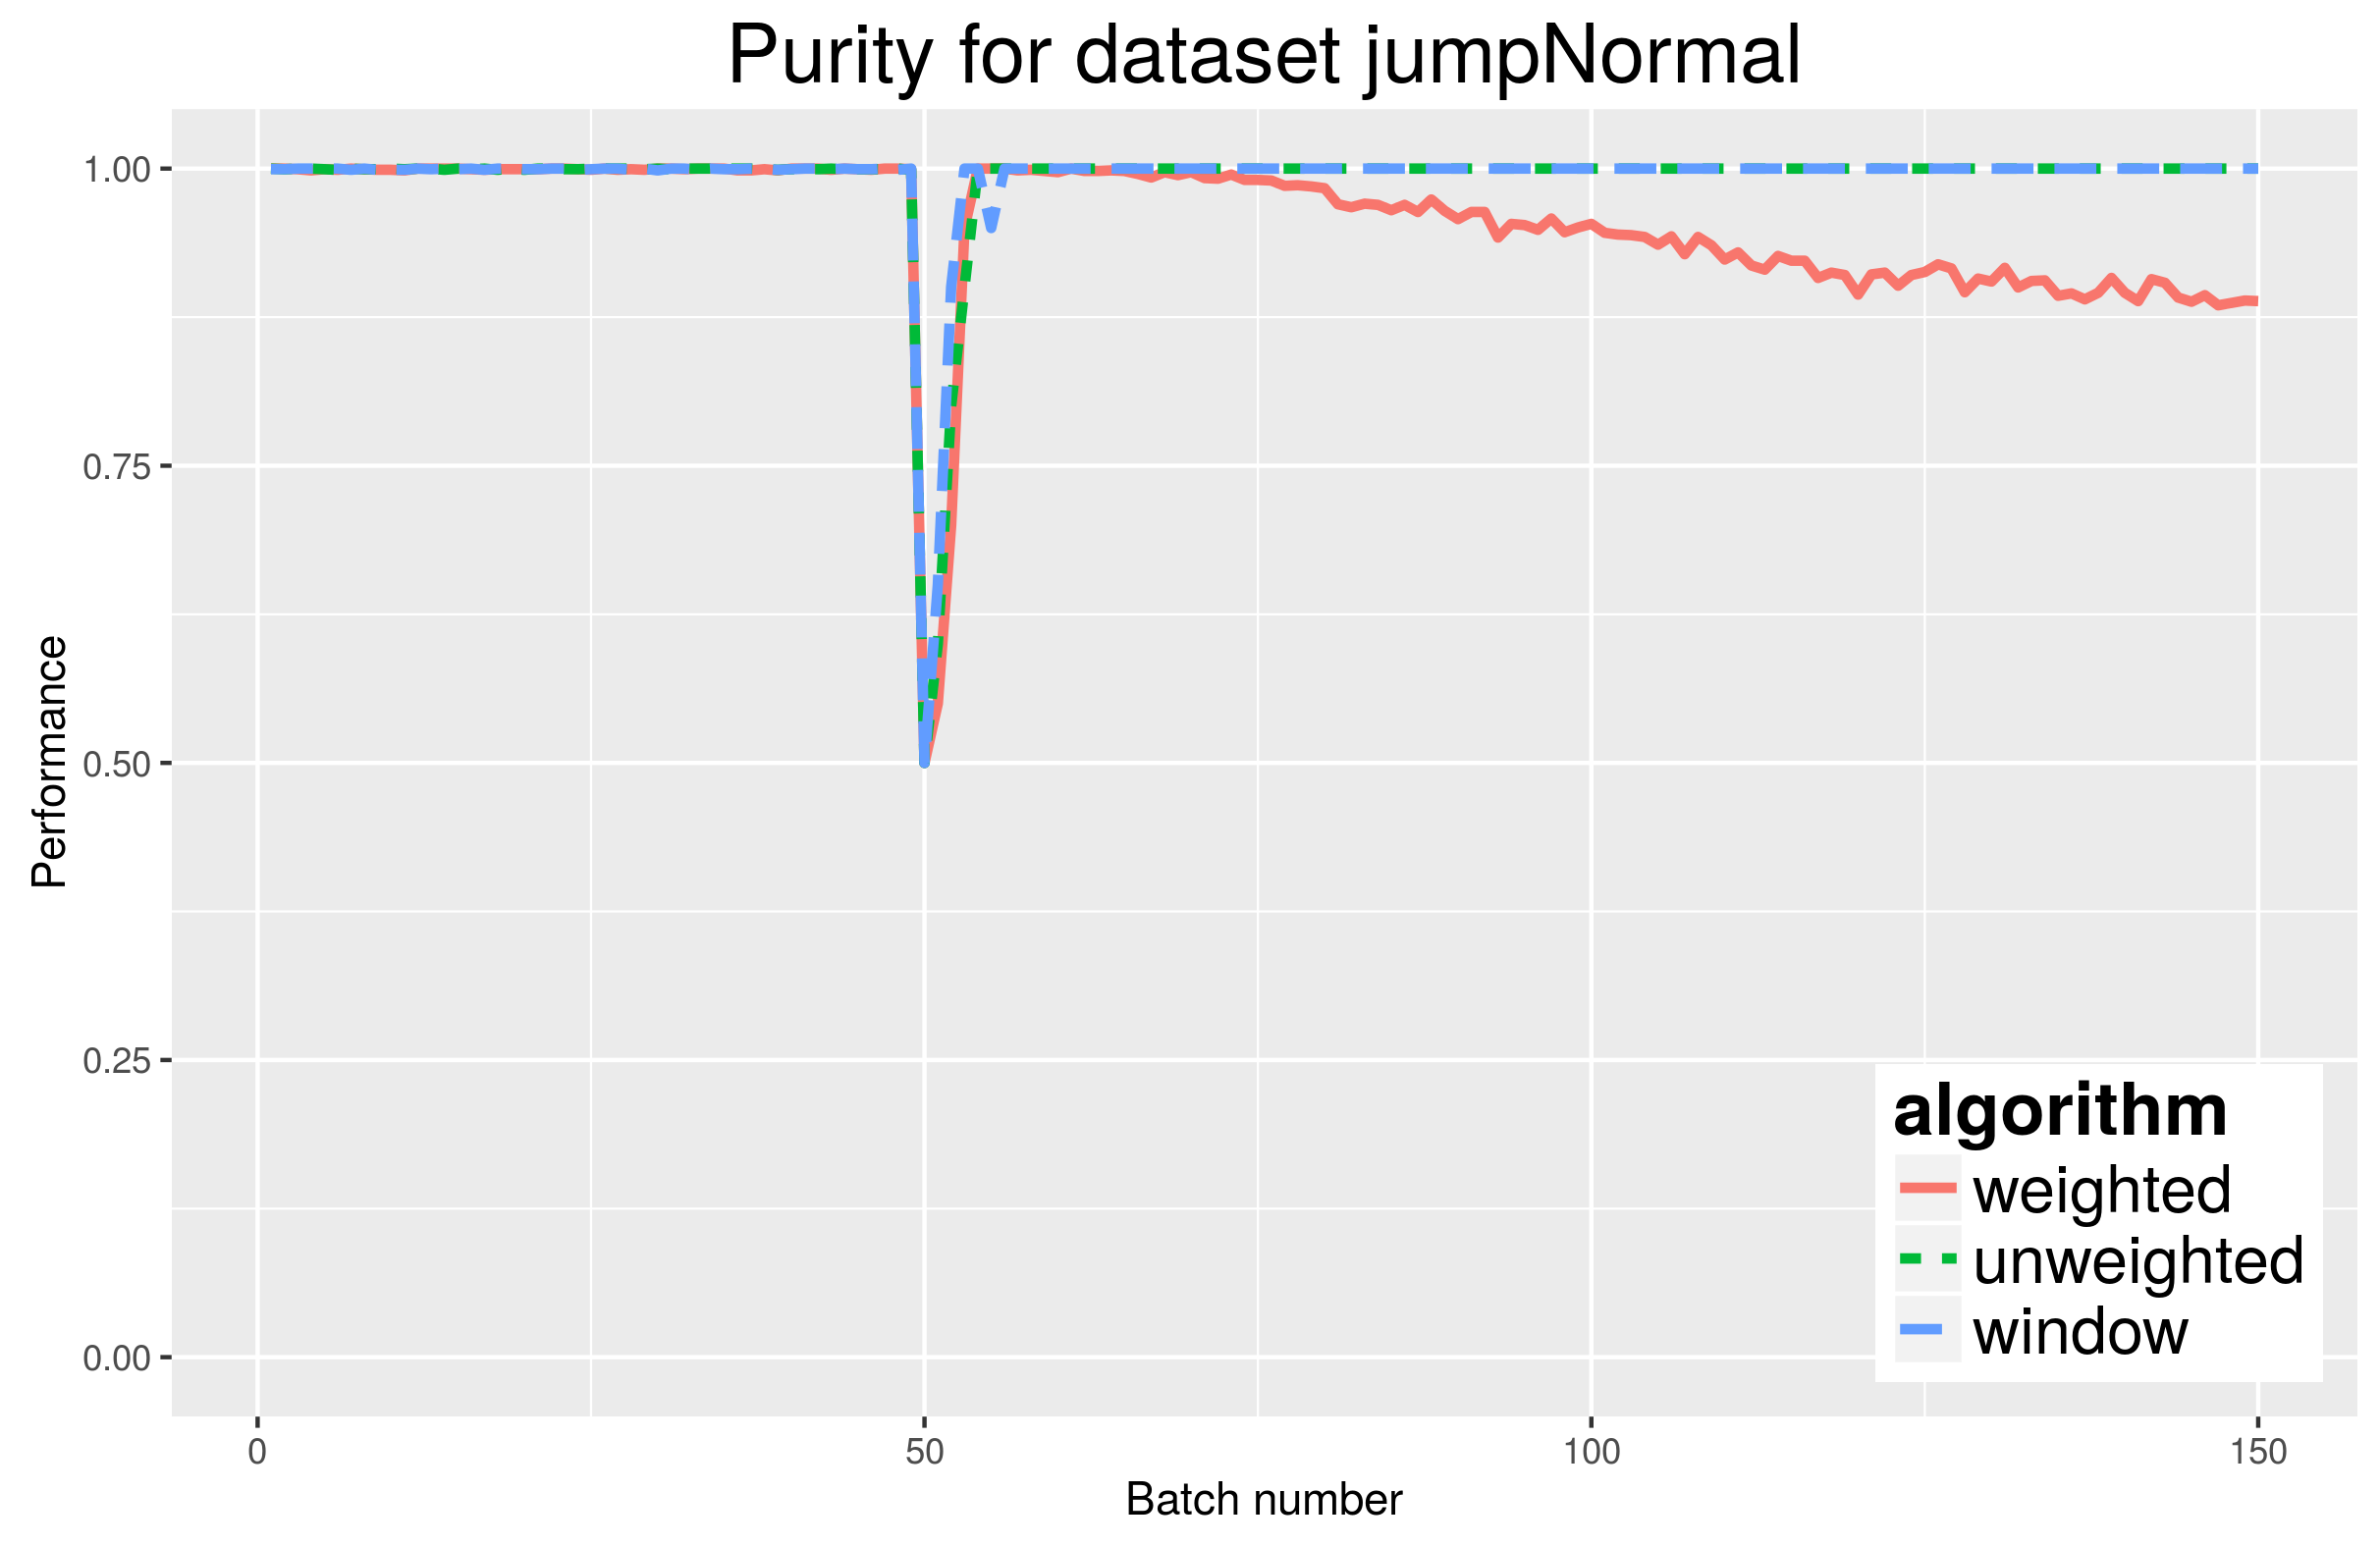
\includegraphics[width=.9\linewidth]{jumpNormal_purity}
  \caption{Jump Normal}
 % \label{fig:sfig1}
\end{subfigure}%
\begin{subfigure}{.5\textwidth}
  \centering
  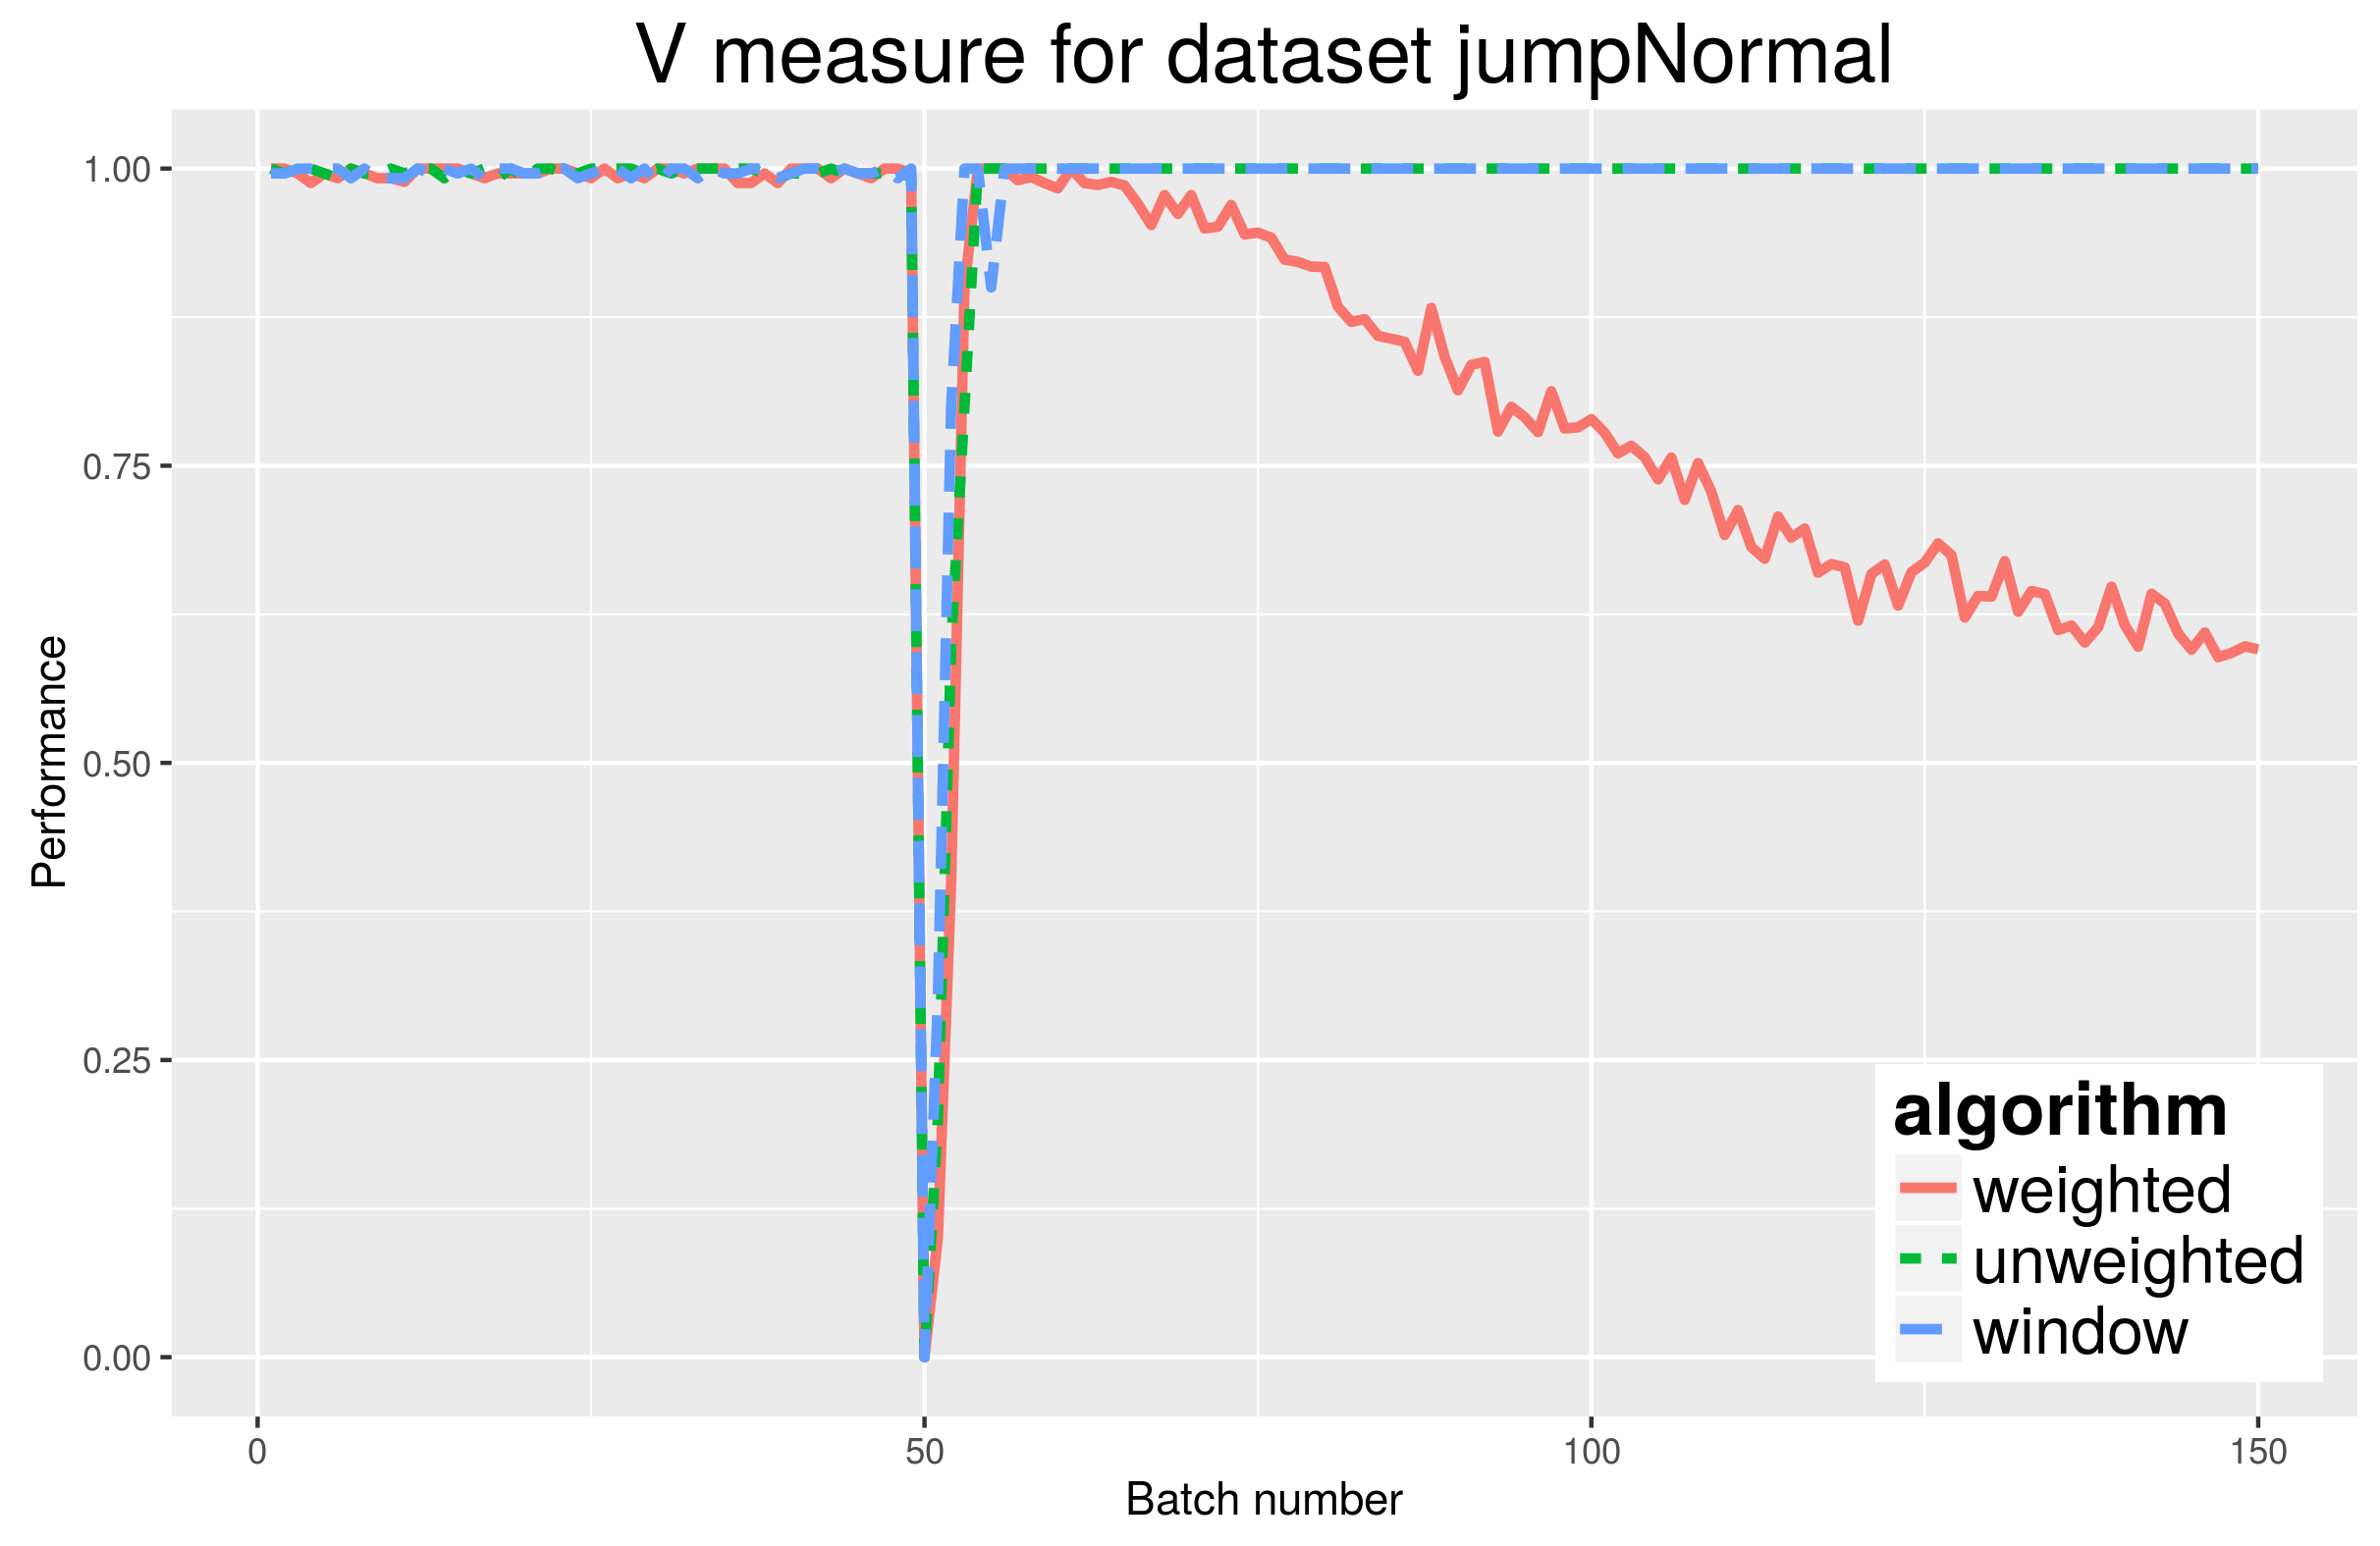
\includegraphics[width=.9\linewidth]{jumpNormal_vmeasure}
  \caption{Jump Normal V-measure}
%  \label{fig:sfig2}
\end{subfigure}
\caption{Performance of Spectral Clustream (weighted and unweighted) and windowed spectral}
\label{fig:simulated_clustream}
\end{figure}

The first thing to note is that unweighted clustream and the windowed algorithm both generally perform excellently on all data sets for the duration of the stream. The gradual drift data set doesn't seem to be too challenging for these algorithms, and although there is a downward spike in the abrupt data set at the point of change, both algorithms  adapt and recover quickly. The weighted version of clustream starts with good performance in all three sets, but rapidly deteriorate as the streams progress, at times dropping to V-measure values of below 0.5.   

\subsection{Real Data Results}

We investigate the performance of Clustream spectral clustering and Windowed Spectral clustering on real data. The data set is taken from the UCI Pendigits data set and consists of hand drawn digits of the numbers 0-9. There are 250 samples taken from 44 writers. The data was collected using a pressure sensitive tablet. There are 16 features, each relating to the co-ordinate information taken from the input tablet. We restrict our analysis to pairwise comparison of digits. For example we attempt to cluster the digits 0 and 1, and treat the data as if it is arriving in a constant data stream. 

The results for a selection of the pairwise digits are shown in Figure \ref{fig:uci_pendigits}. The first column displays the digit data in PCA space, the second column shows the purity, and the third column shows the V-measure. The pendigit data is more challenging than the simulated data, however both windowed spectral and the unweighted spectral clustream generally do well. Again we observe that weighted Clustream has poor performance, and it seems that once the performance drops, it struggles to improve again. Interestingly, occasionally windowed spectral clustering seems to heavily drop in performance, making a bad clustering, but it recovers quickly due to the nature of the relatively small window size. 


\begin{figure}[H]
\begin{subfigure}{.3\textwidth}
  \centering
  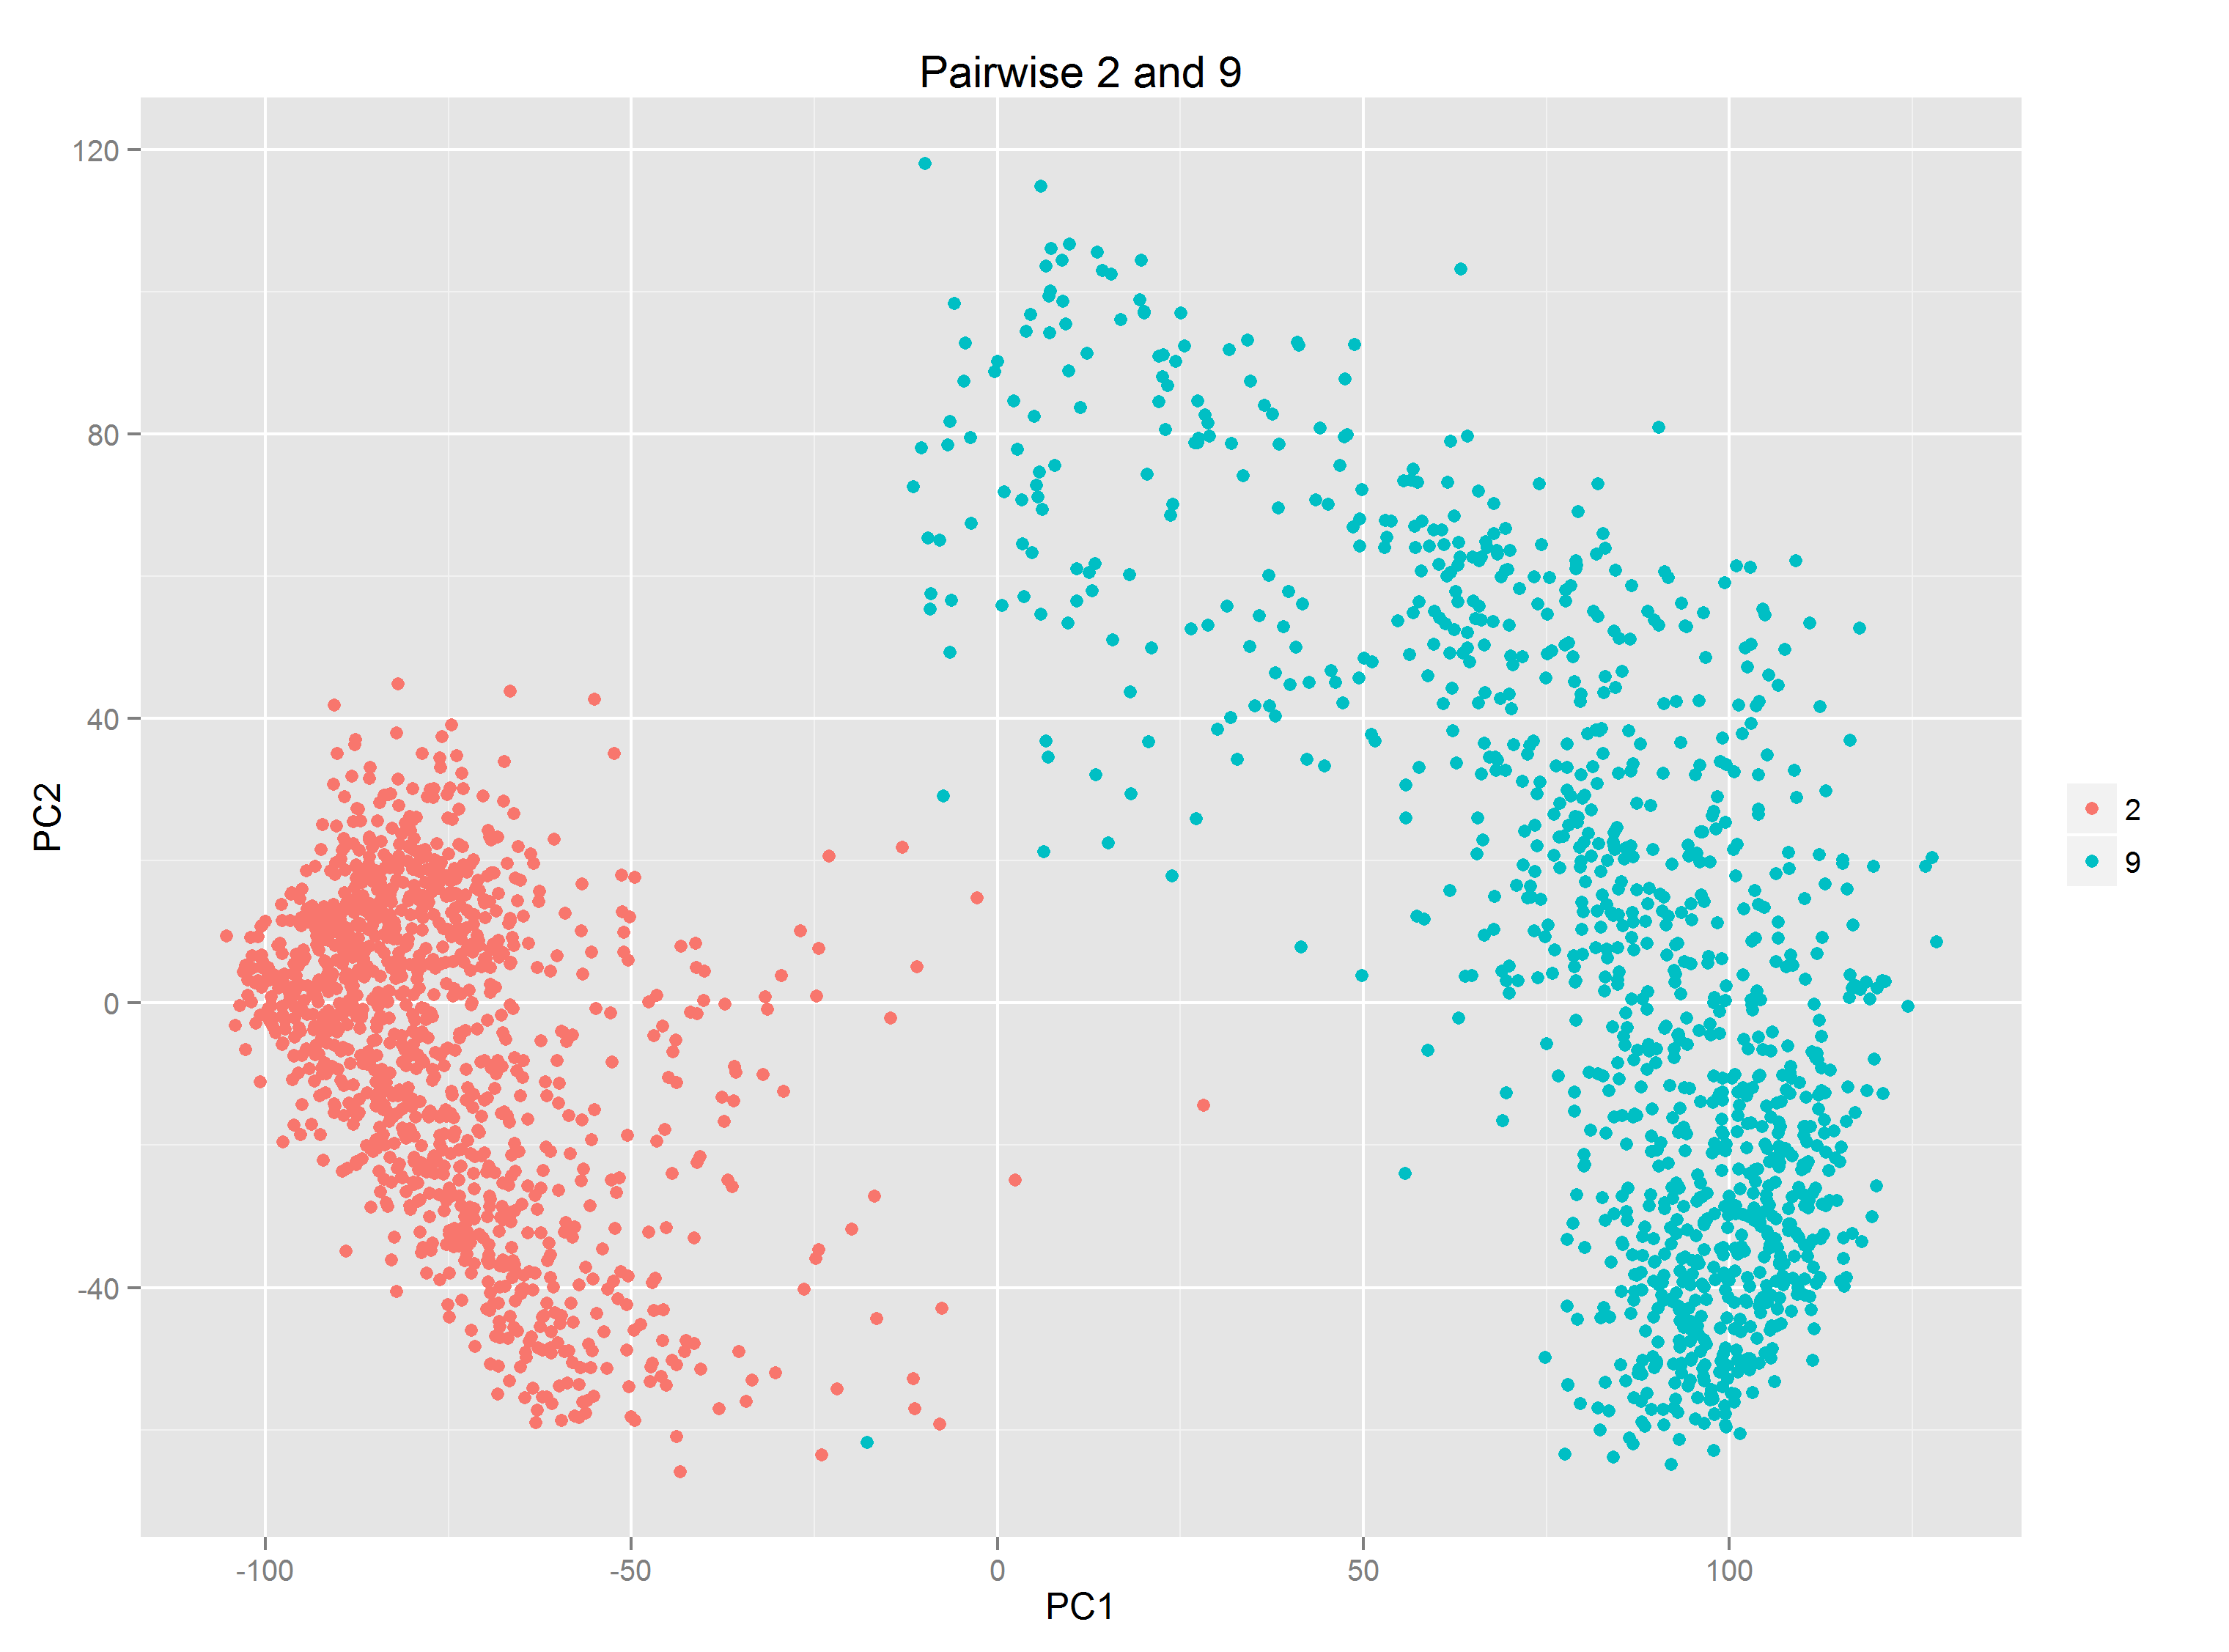
\includegraphics[width=.8\linewidth]{PCA_pendigits_pairwise/pairwise_2_9.png}
  \caption{PCA of digits 2 and 9}
 % \label{fig:sfig1}
\end{subfigure}%
\begin{subfigure}{.3\textwidth}
  \centering
  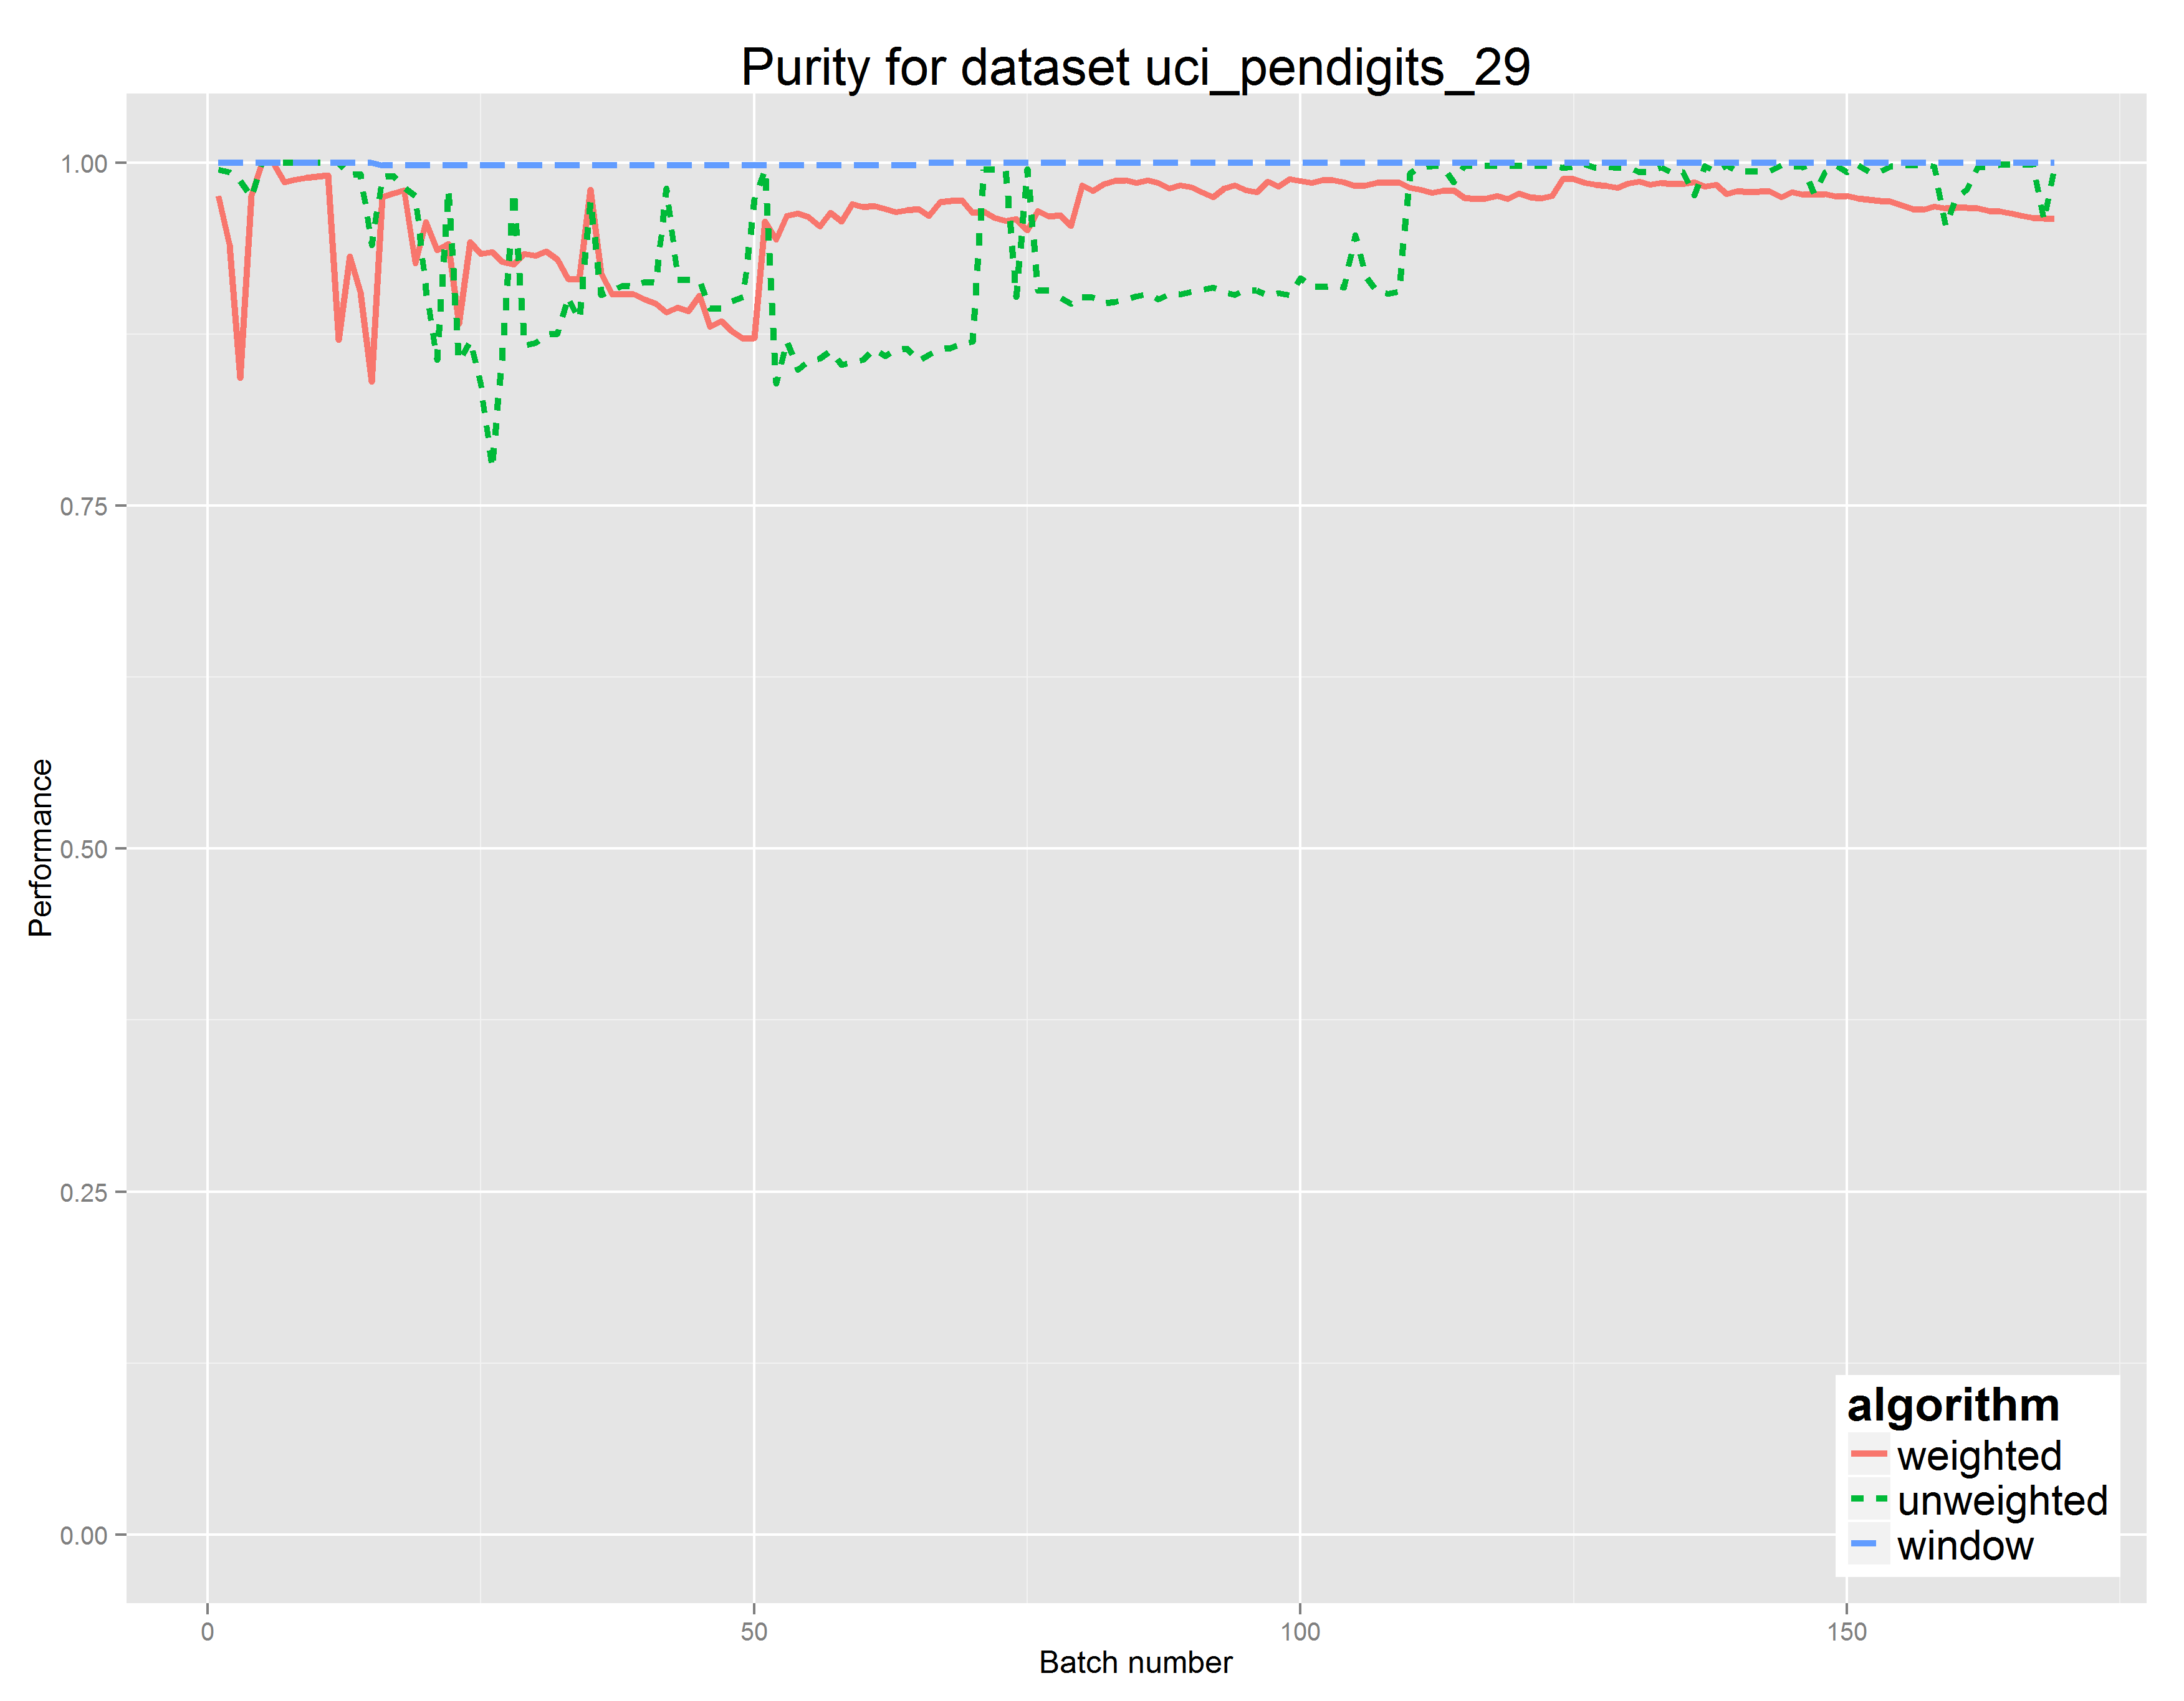
\includegraphics[width=.8\linewidth]{pendigit_results_2016_08_16/uci_pendigits_29_purity.png}
  \caption{Purity digits 2 and 9}
%  \label{fig:sfig2}
\end{subfigure}
\begin{subfigure}{.3\textwidth}
  \centering
  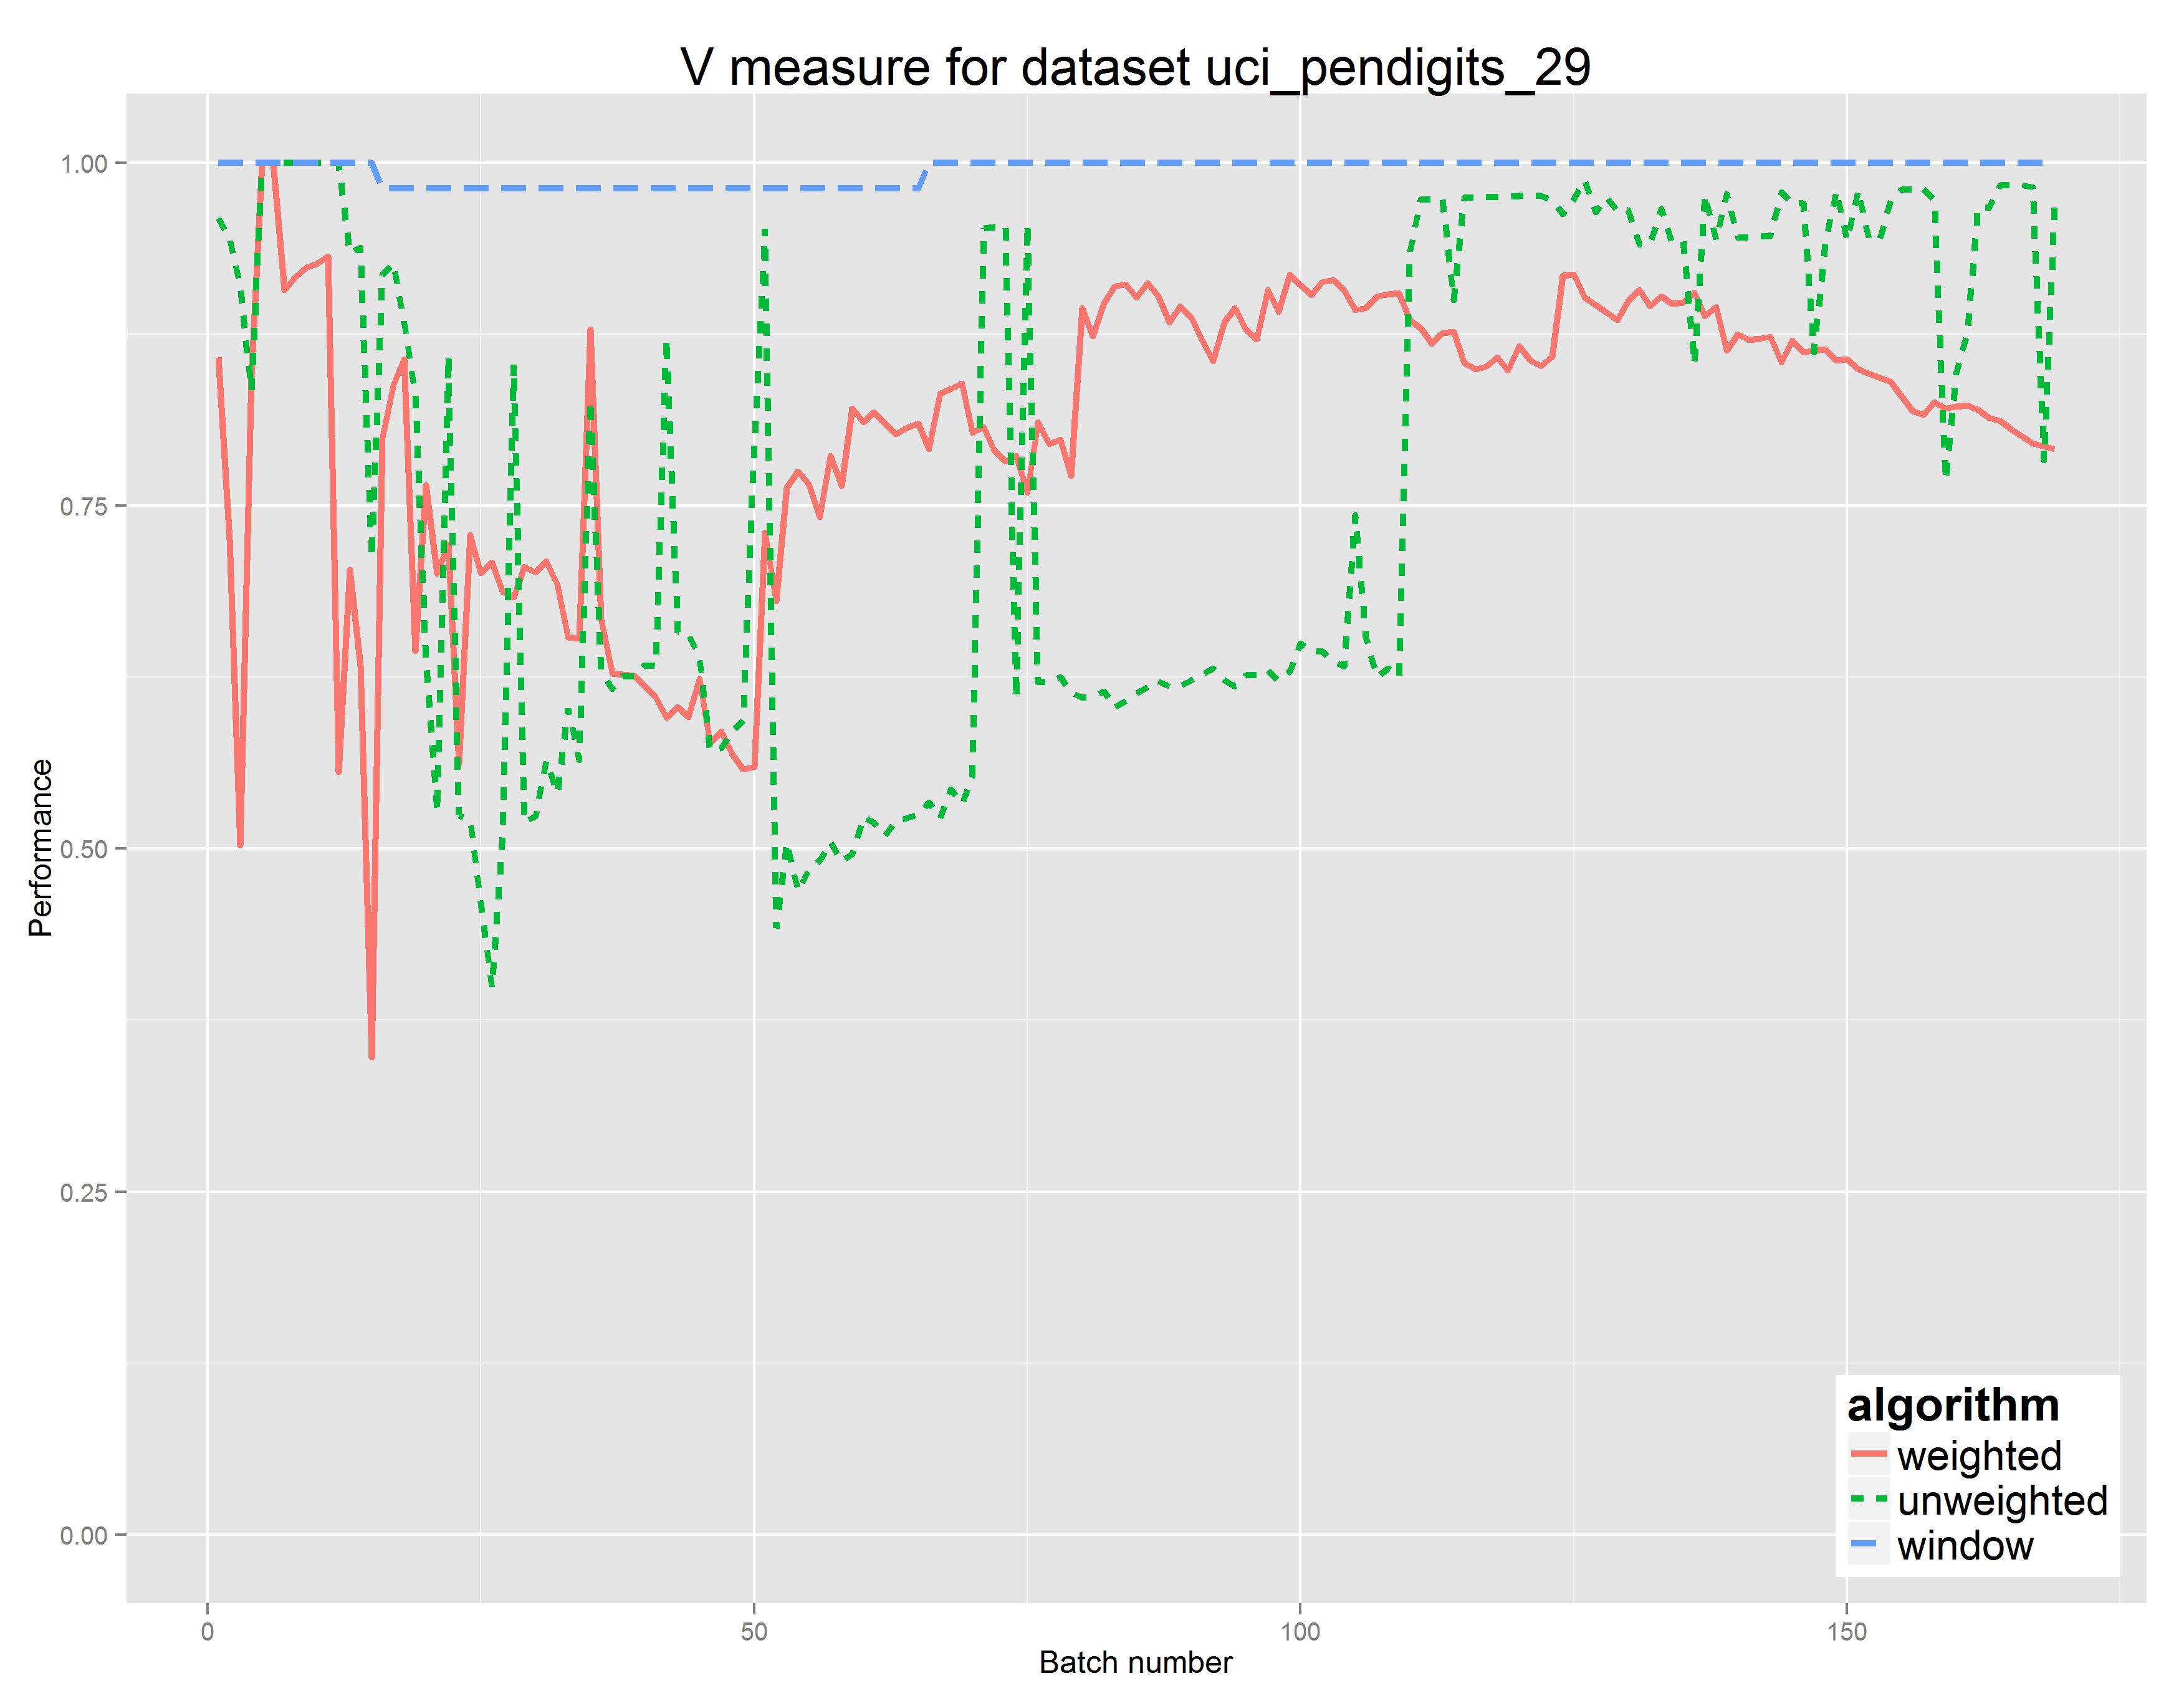
\includegraphics[width=.8\linewidth]{pendigit_results_2016_08_16/uci_pendigits_29_vmeasure.png}
  \caption{V-measure digits 2 and 9}
%  \label{fig:sfig2}
\end{subfigure}


\begin{subfigure}{.3\textwidth}
  \centering
  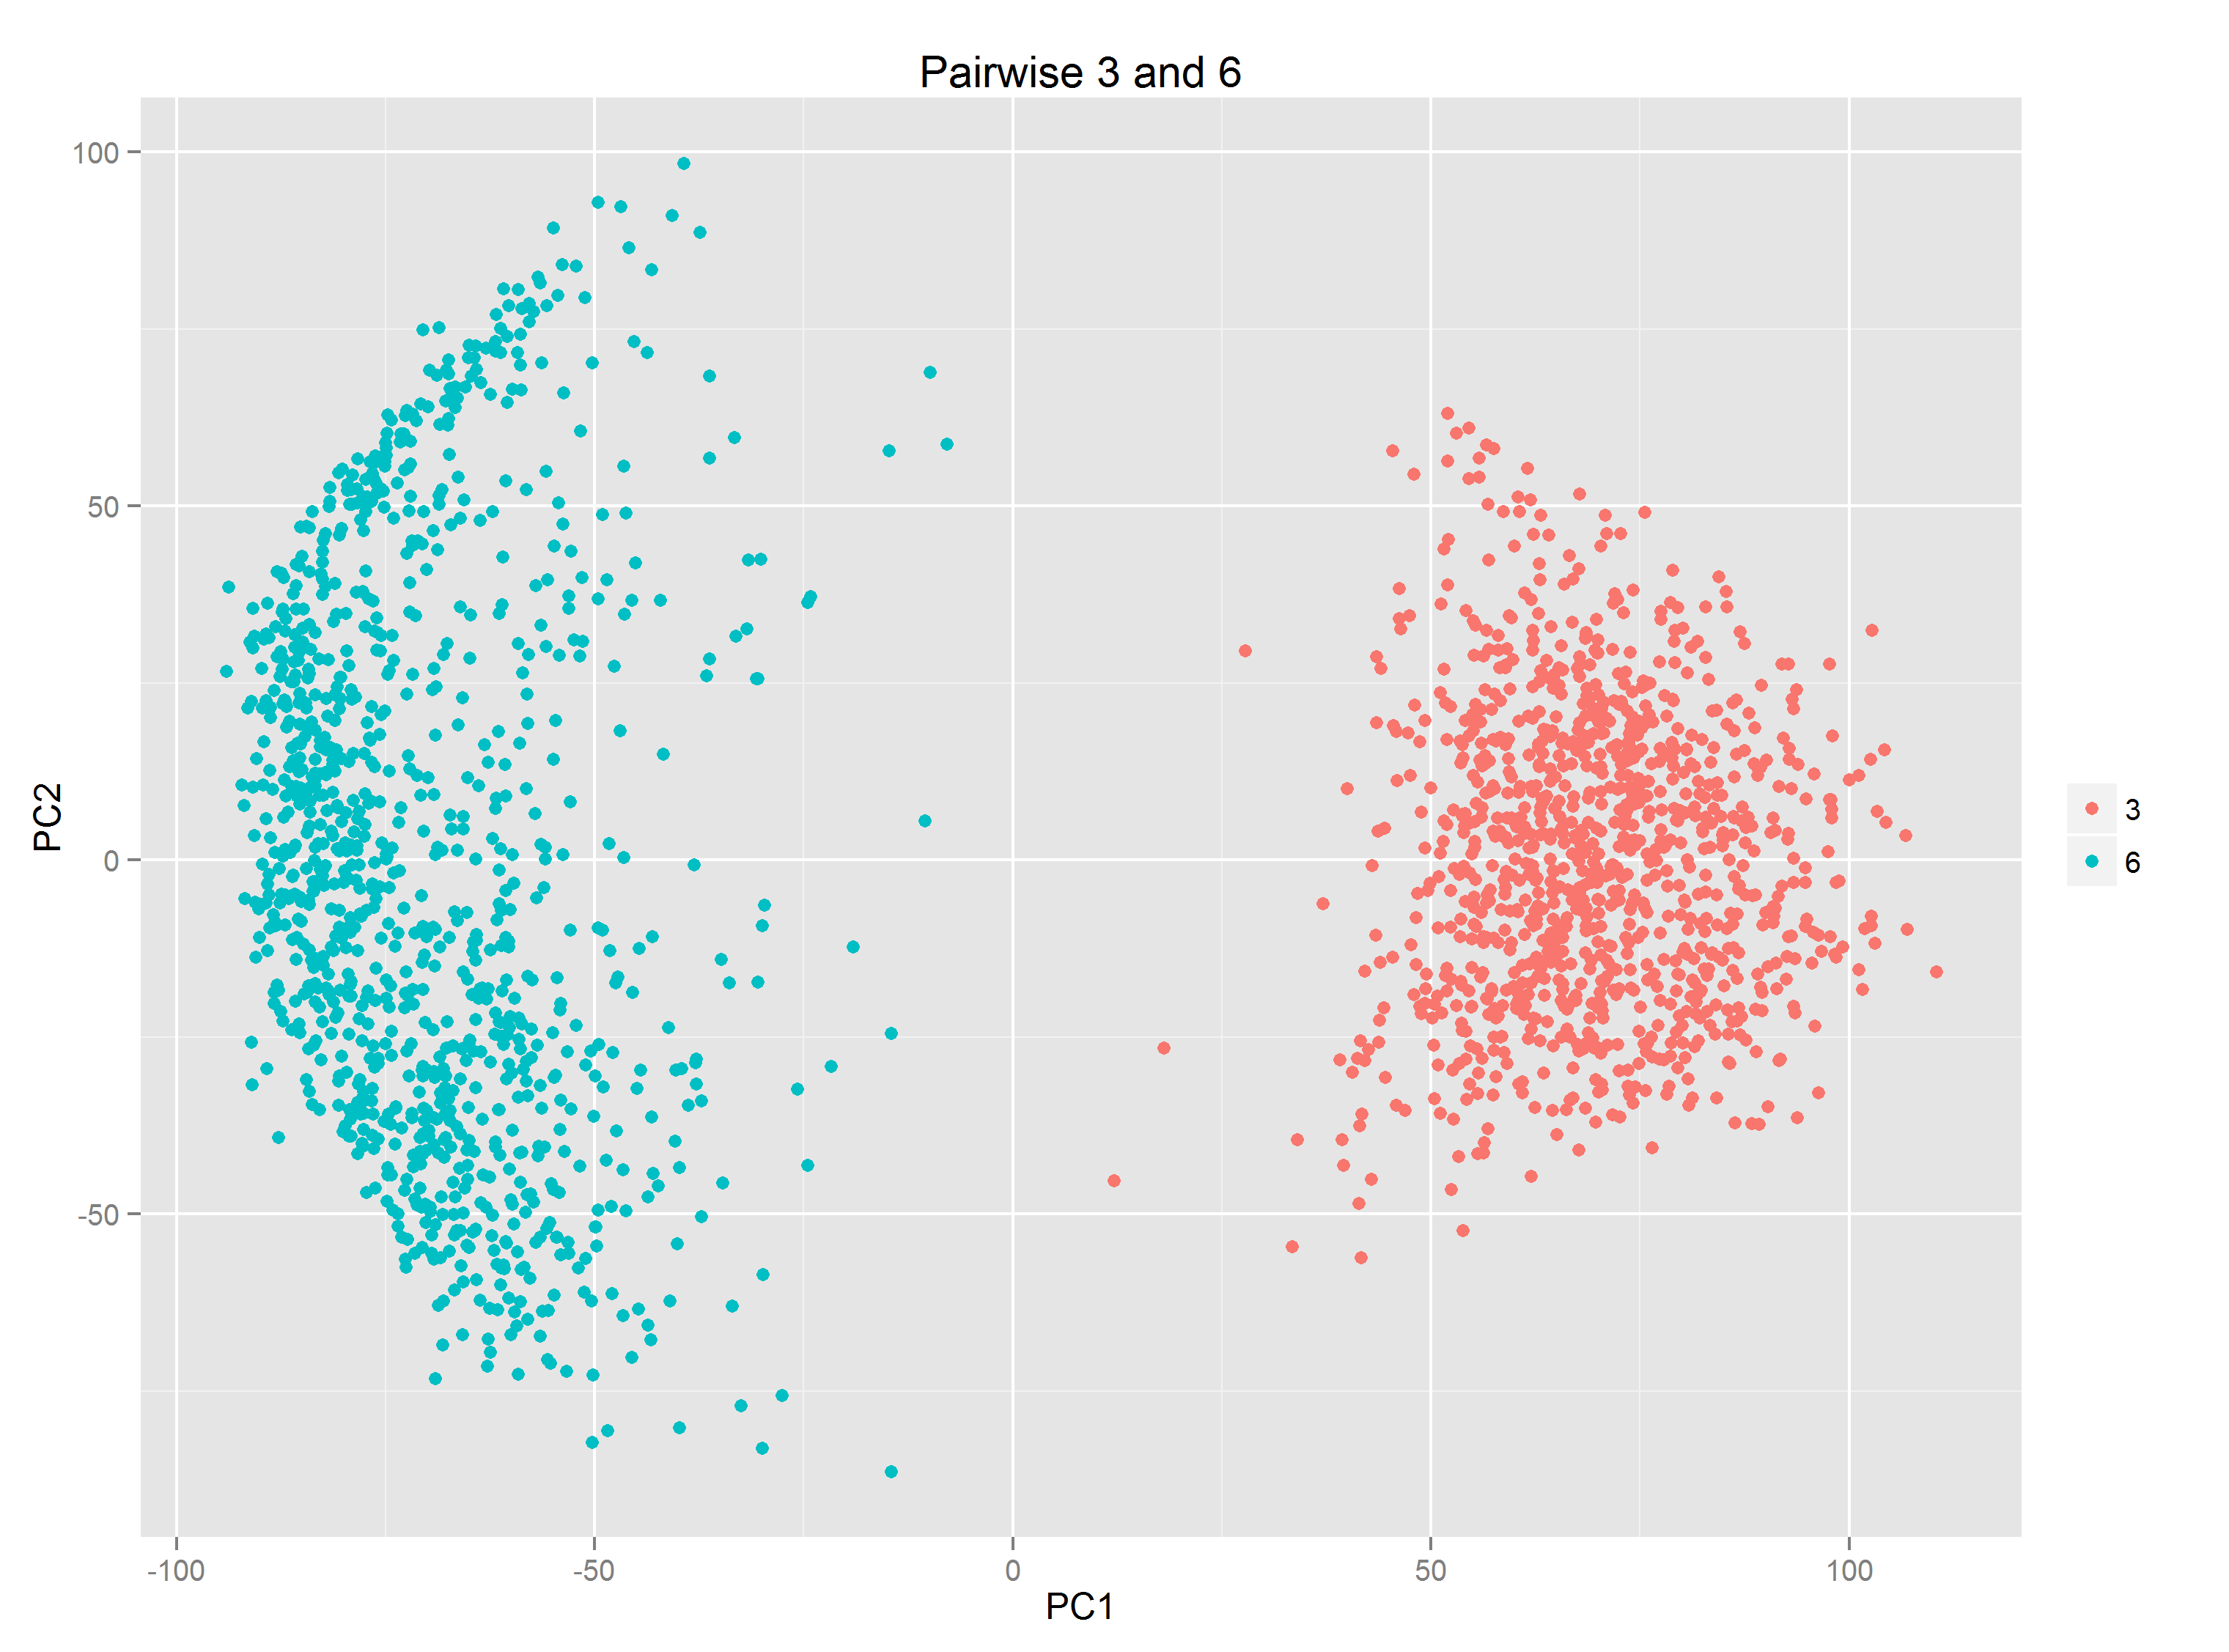
\includegraphics[width=.8\linewidth]{PCA_pendigits_pairwise/pairwise_3_6.png}
  \caption{PCA of digits 3 and 6}
 % \label{fig:sfig1}
\end{subfigure}%
\begin{subfigure}{.3\textwidth}
  \centering
  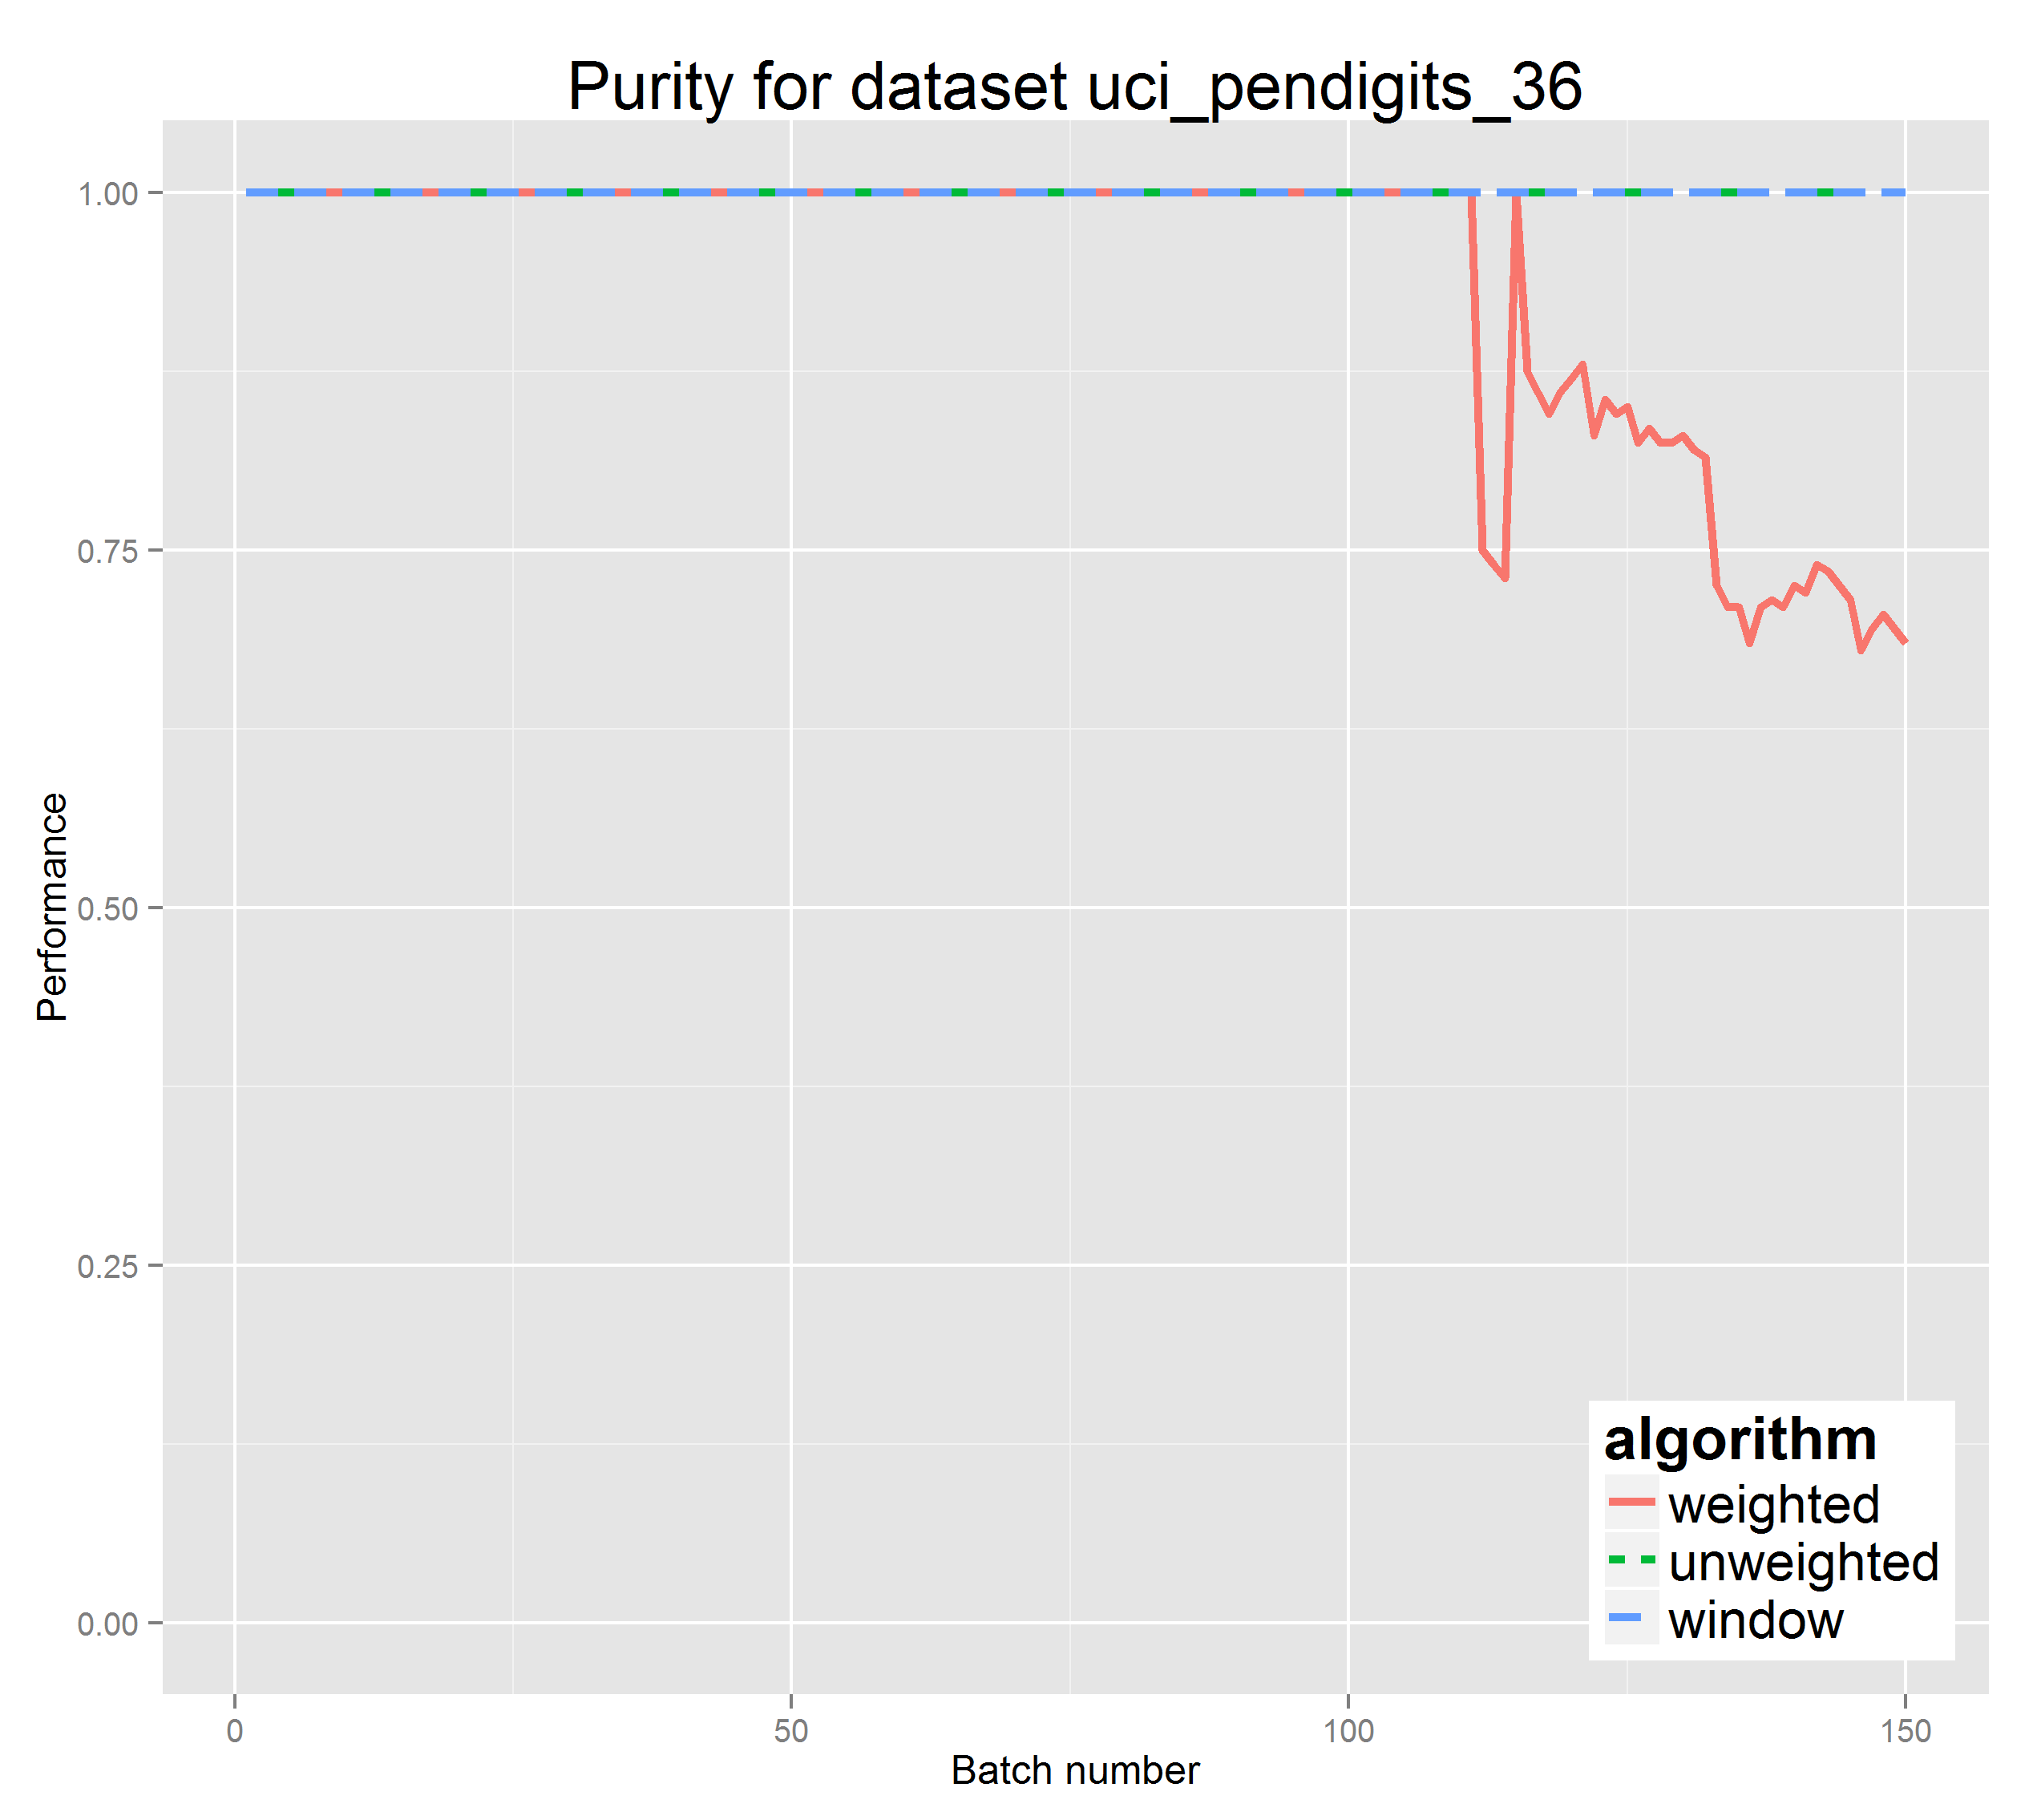
\includegraphics[width=.8\linewidth]{pendigit_results_2016_08_16/uci_pendigits_36_purity.png}
  \caption{Purity digits 3 and 6}
%  \label{fig:sfig2}
\end{subfigure}
\begin{subfigure}{.3\textwidth}
  \centering
  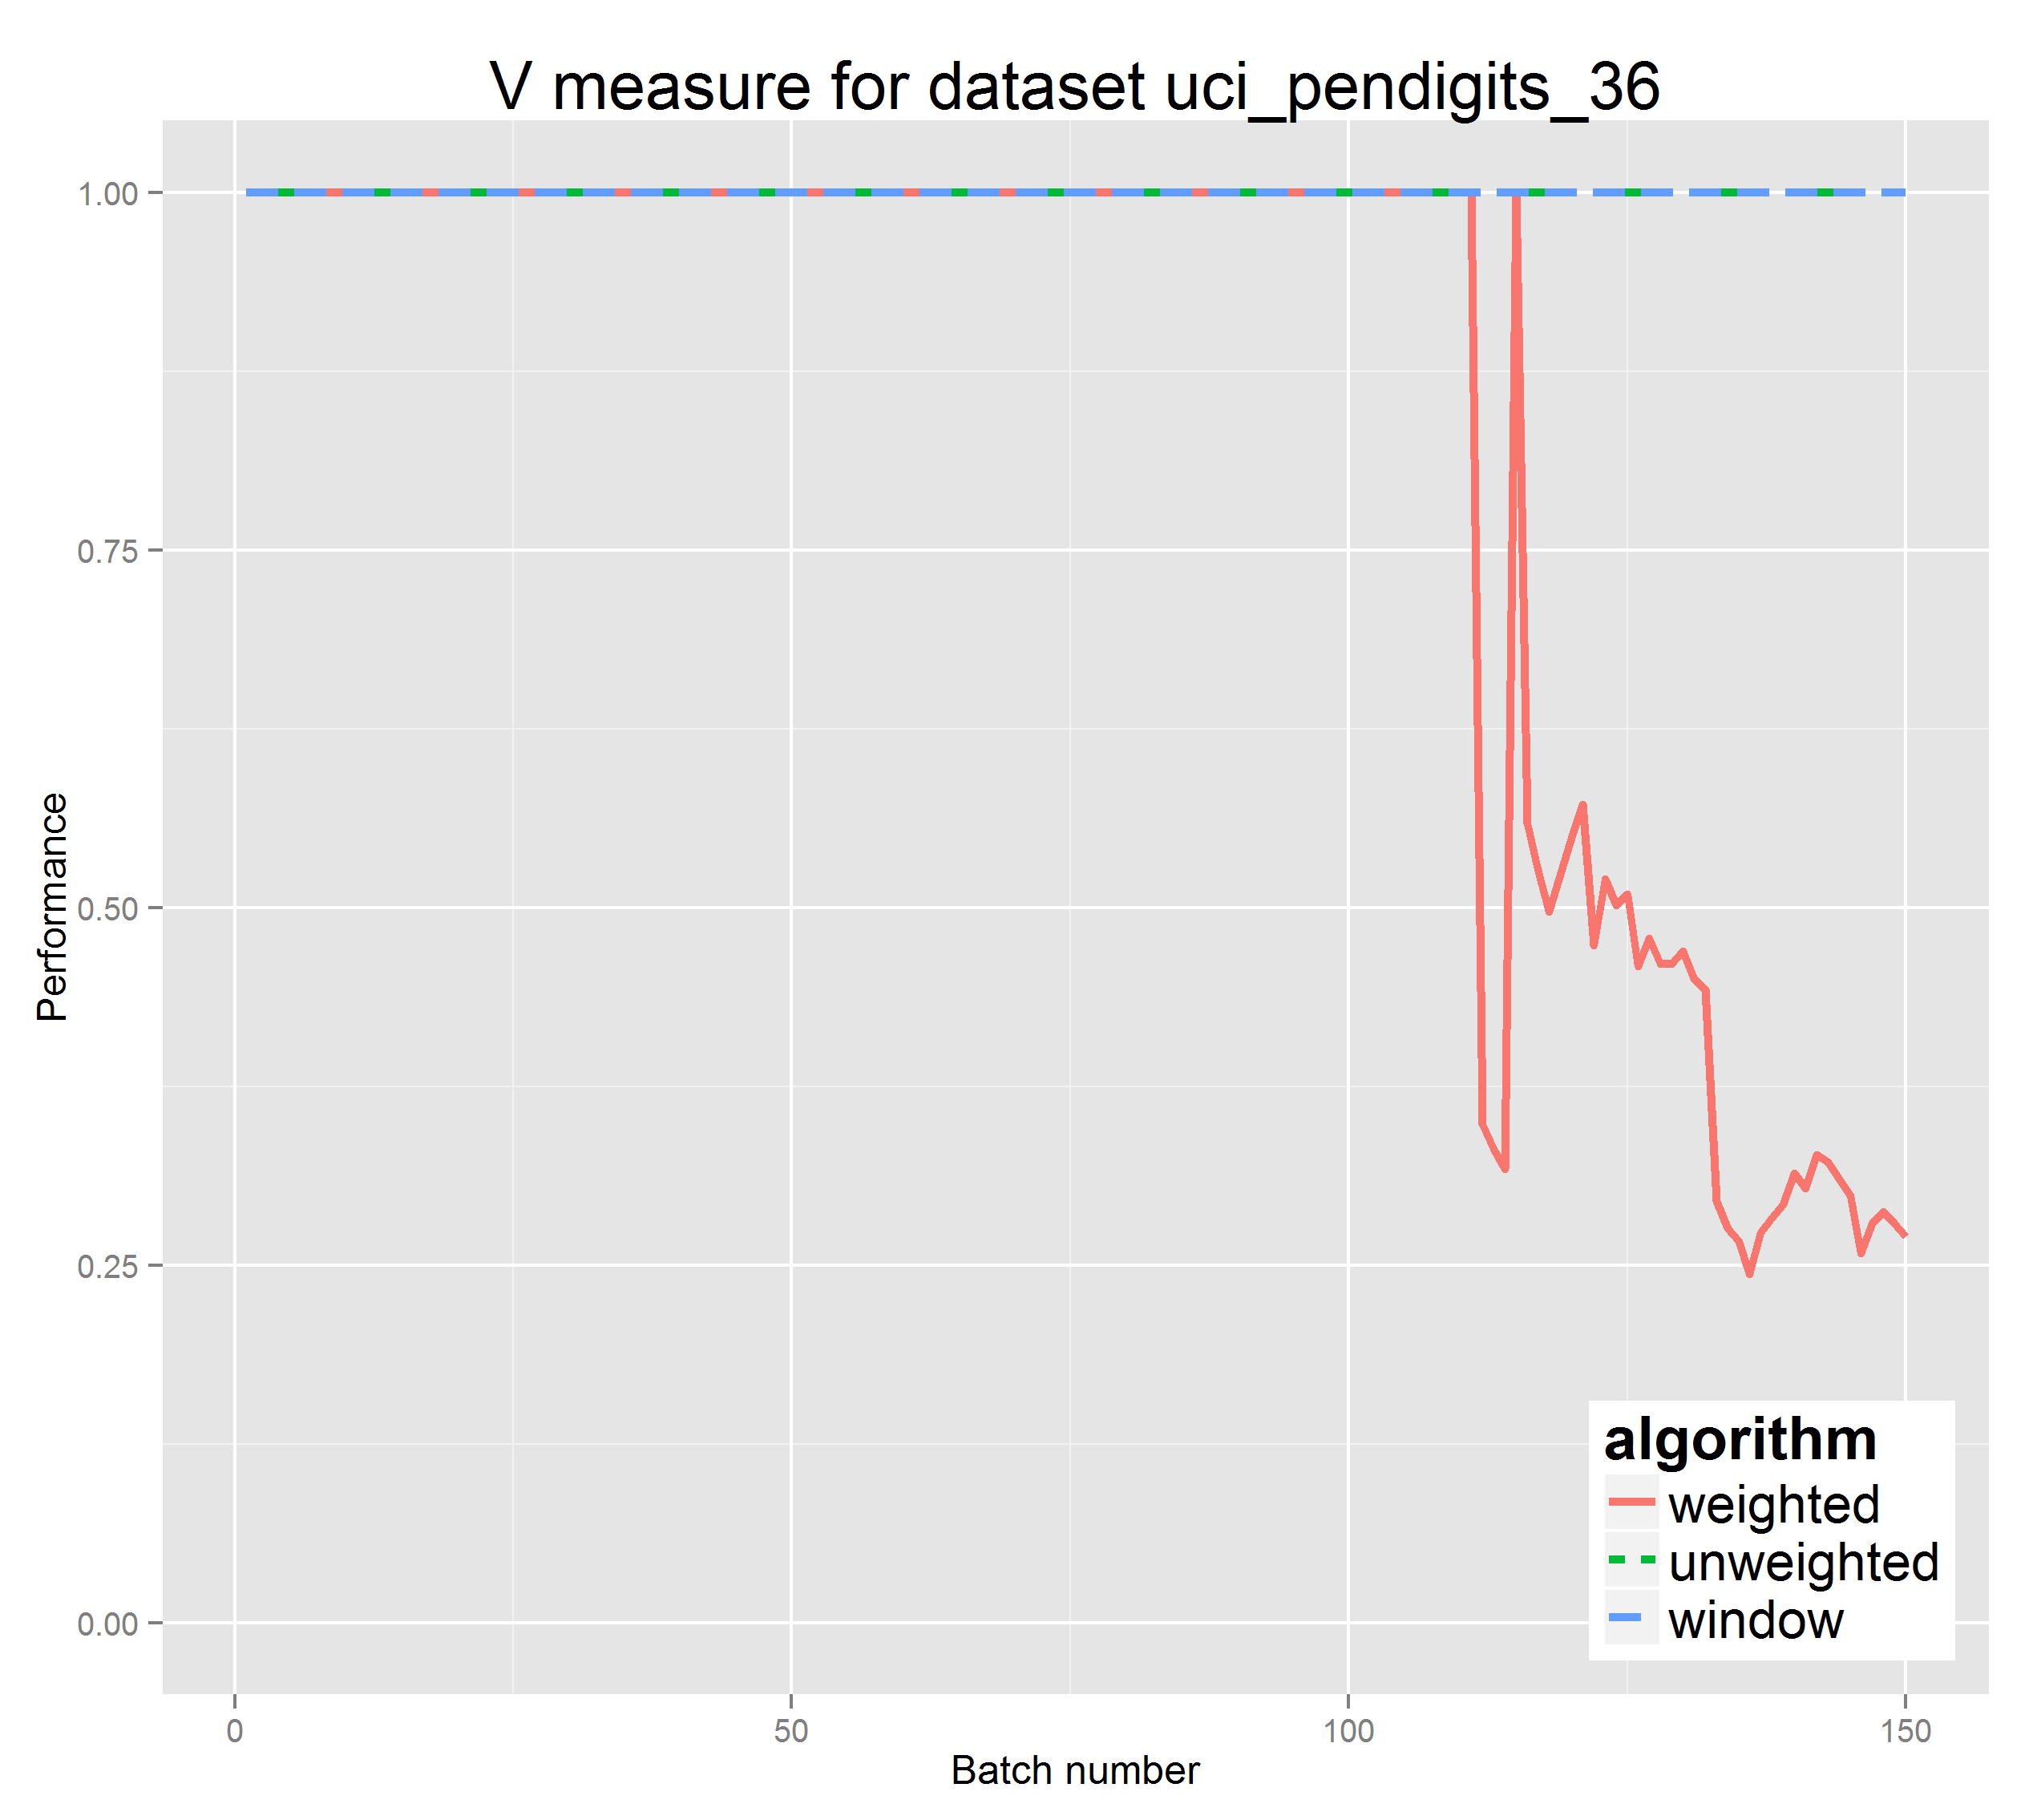
\includegraphics[width=.8\linewidth]{pendigit_results_2016_08_16/uci_pendigits_36_vmeasure.png}
  \caption{V-measure digits 3 and 6}
%  \label{fig:sfig2}
\end{subfigure}

\begin{subfigure}{.3\textwidth}
  \centering
  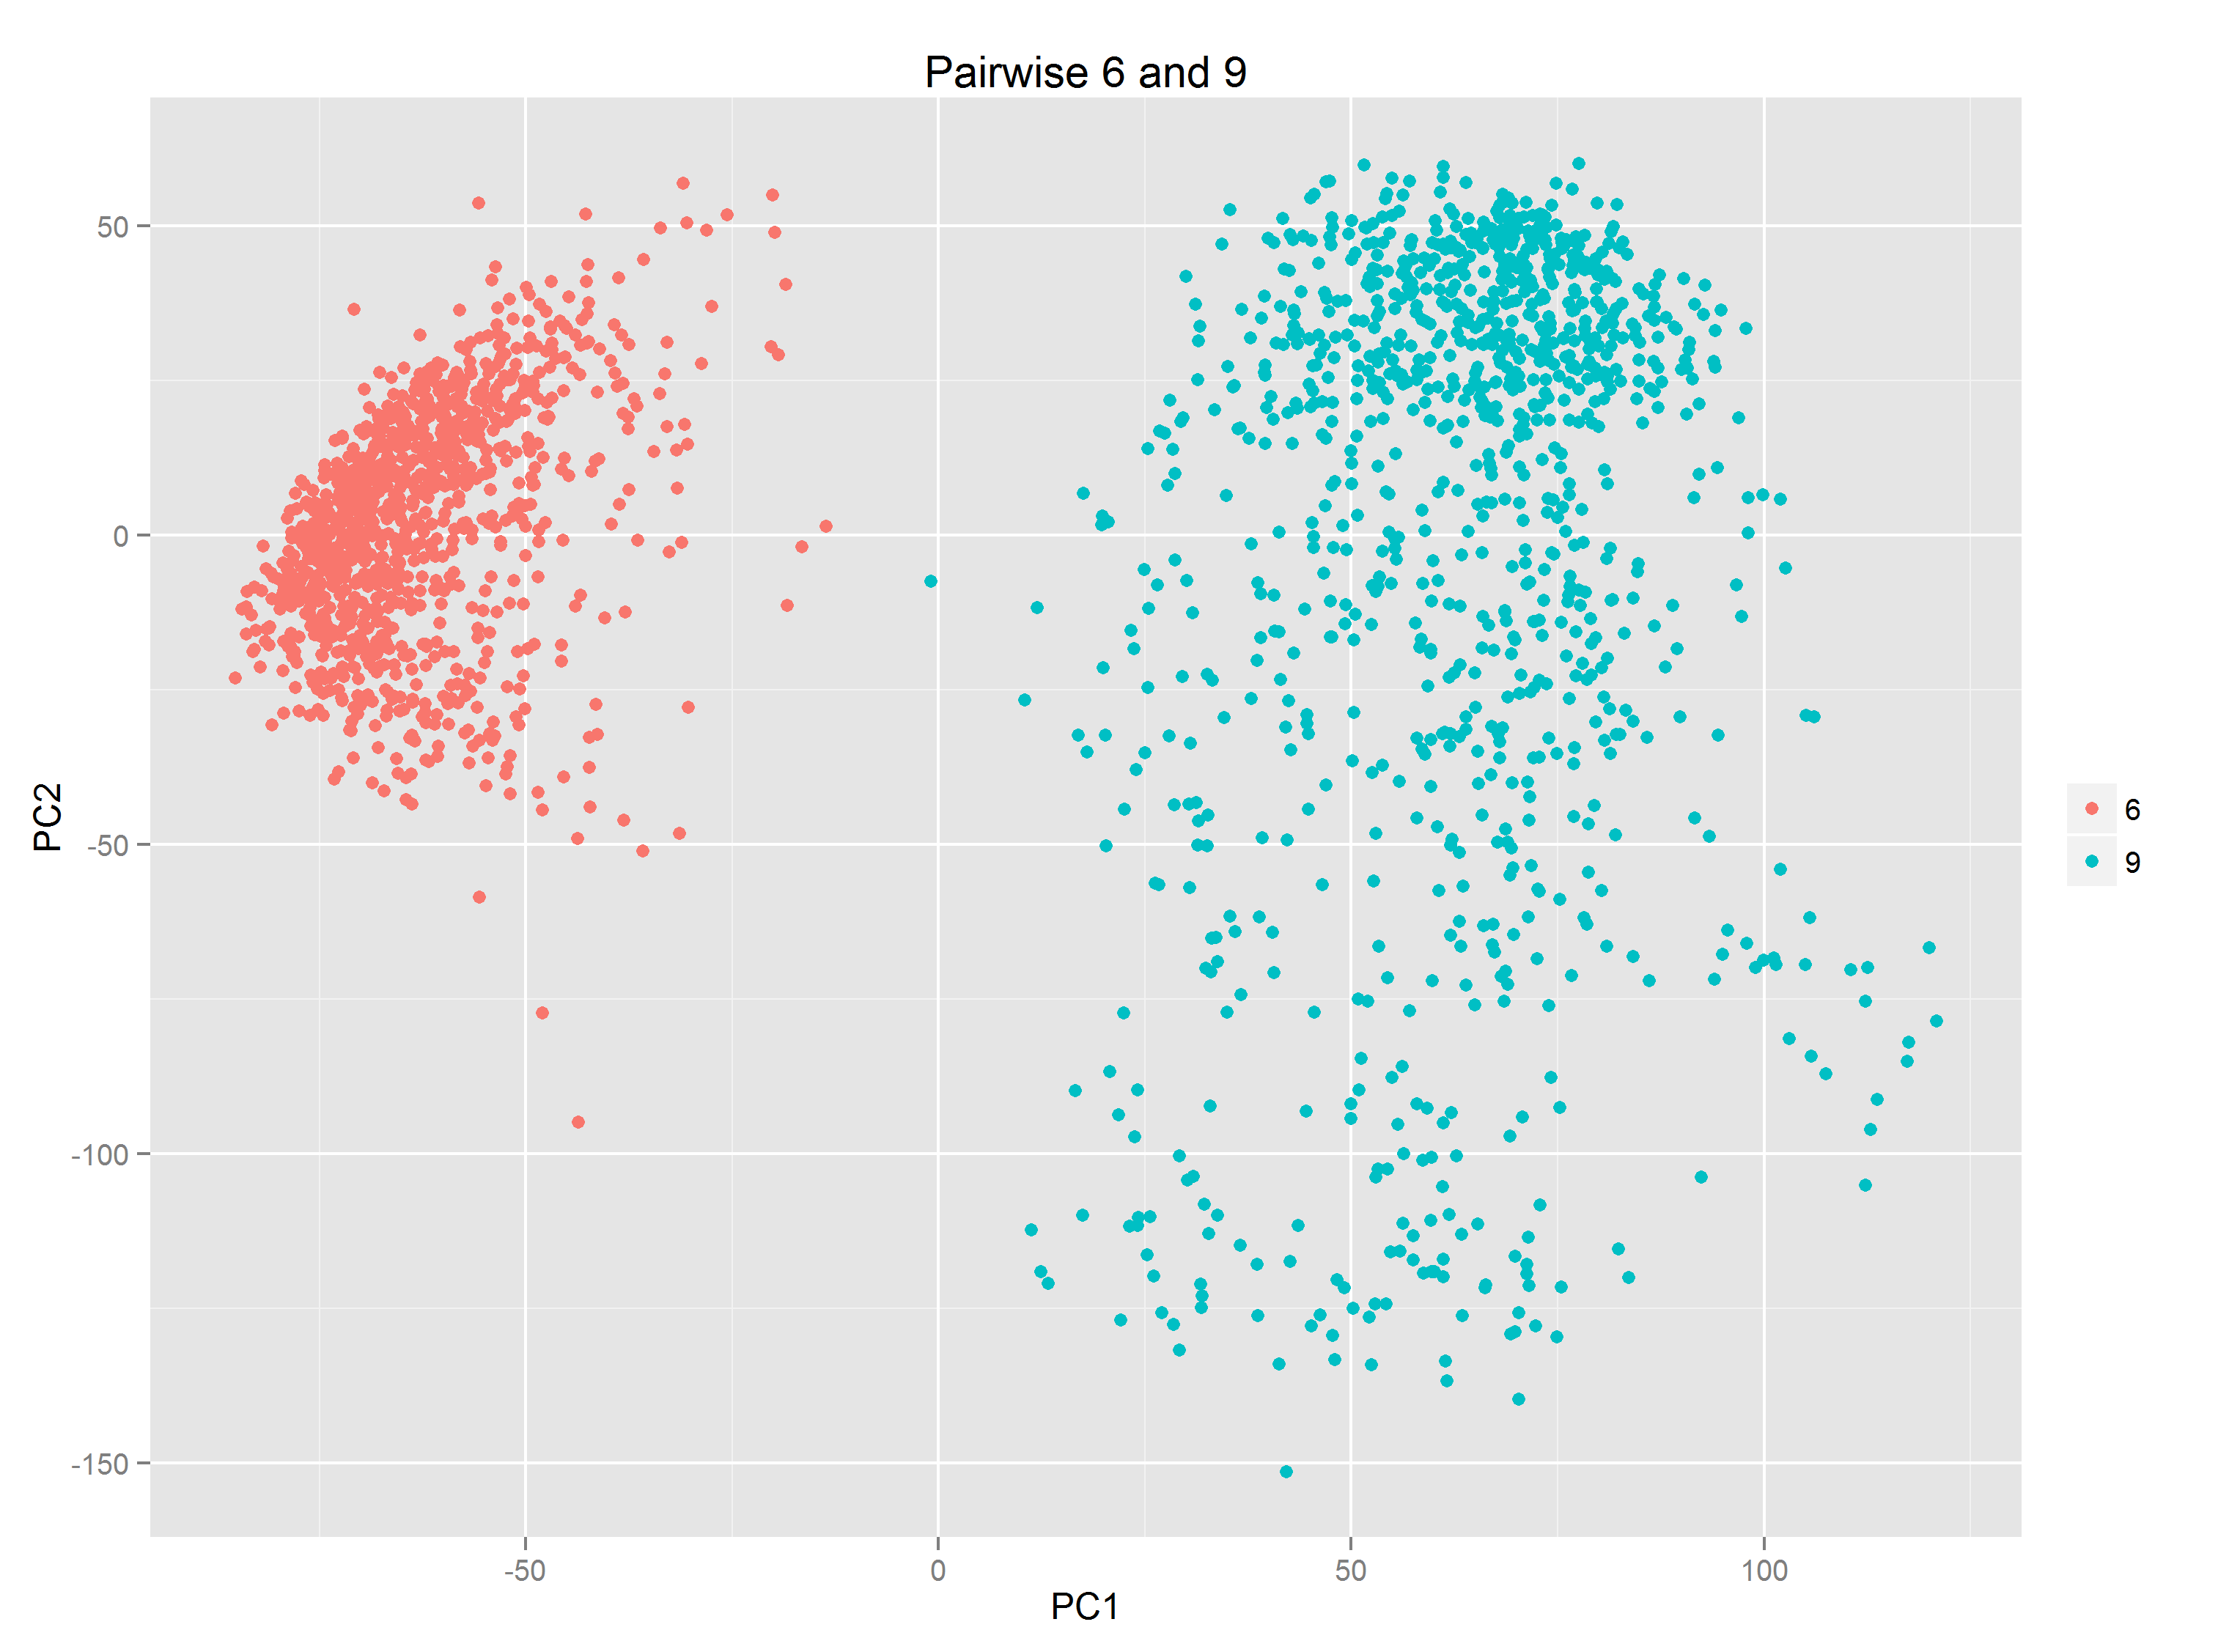
\includegraphics[width=.8\linewidth]{PCA_pendigits_pairwise/pairwise_6_9.png}
  \caption{PCA of digits 6 and 9}
 % \label{fig:sfig1}
\end{subfigure}%
\begin{subfigure}{.3\textwidth}
  \centering
  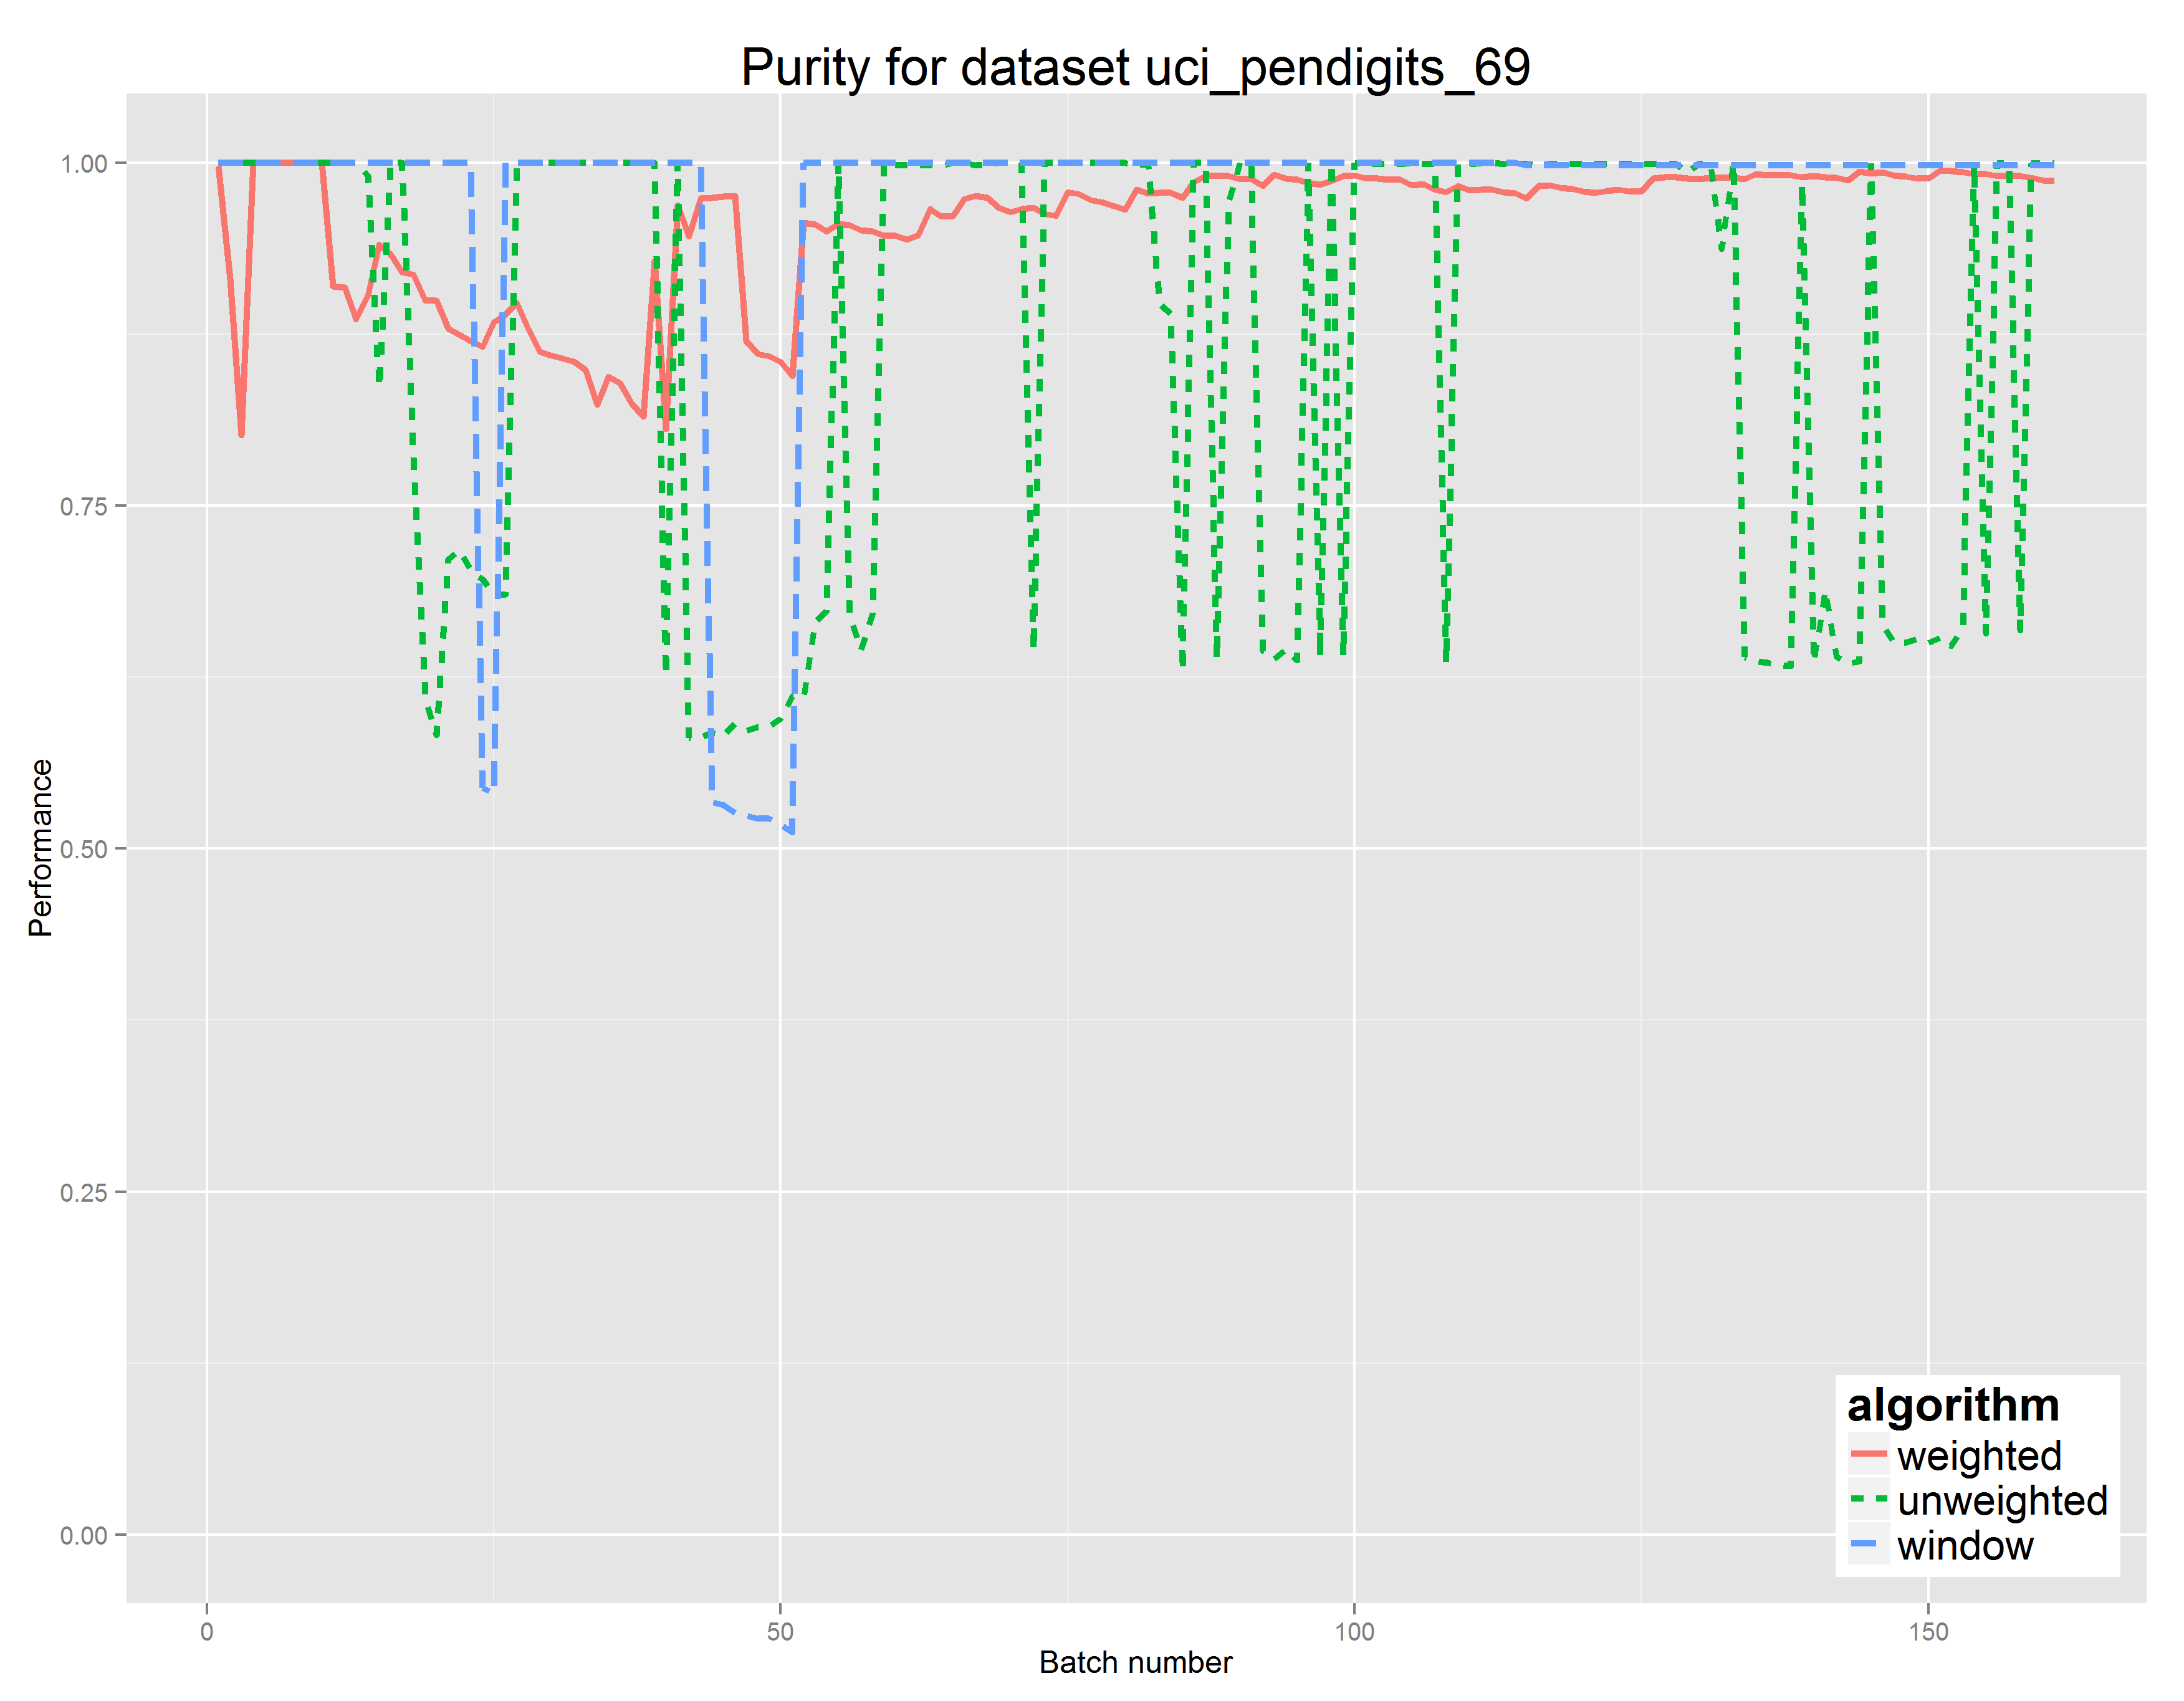
\includegraphics[width=.8\linewidth]{pendigit_results_2016_08_16/uci_pendigits_69_purity.png}
  \caption{Purity digits 6 and 9}
%  \label{fig:sfig2}
\end{subfigure}
\begin{subfigure}{.3\textwidth}
  \centering
  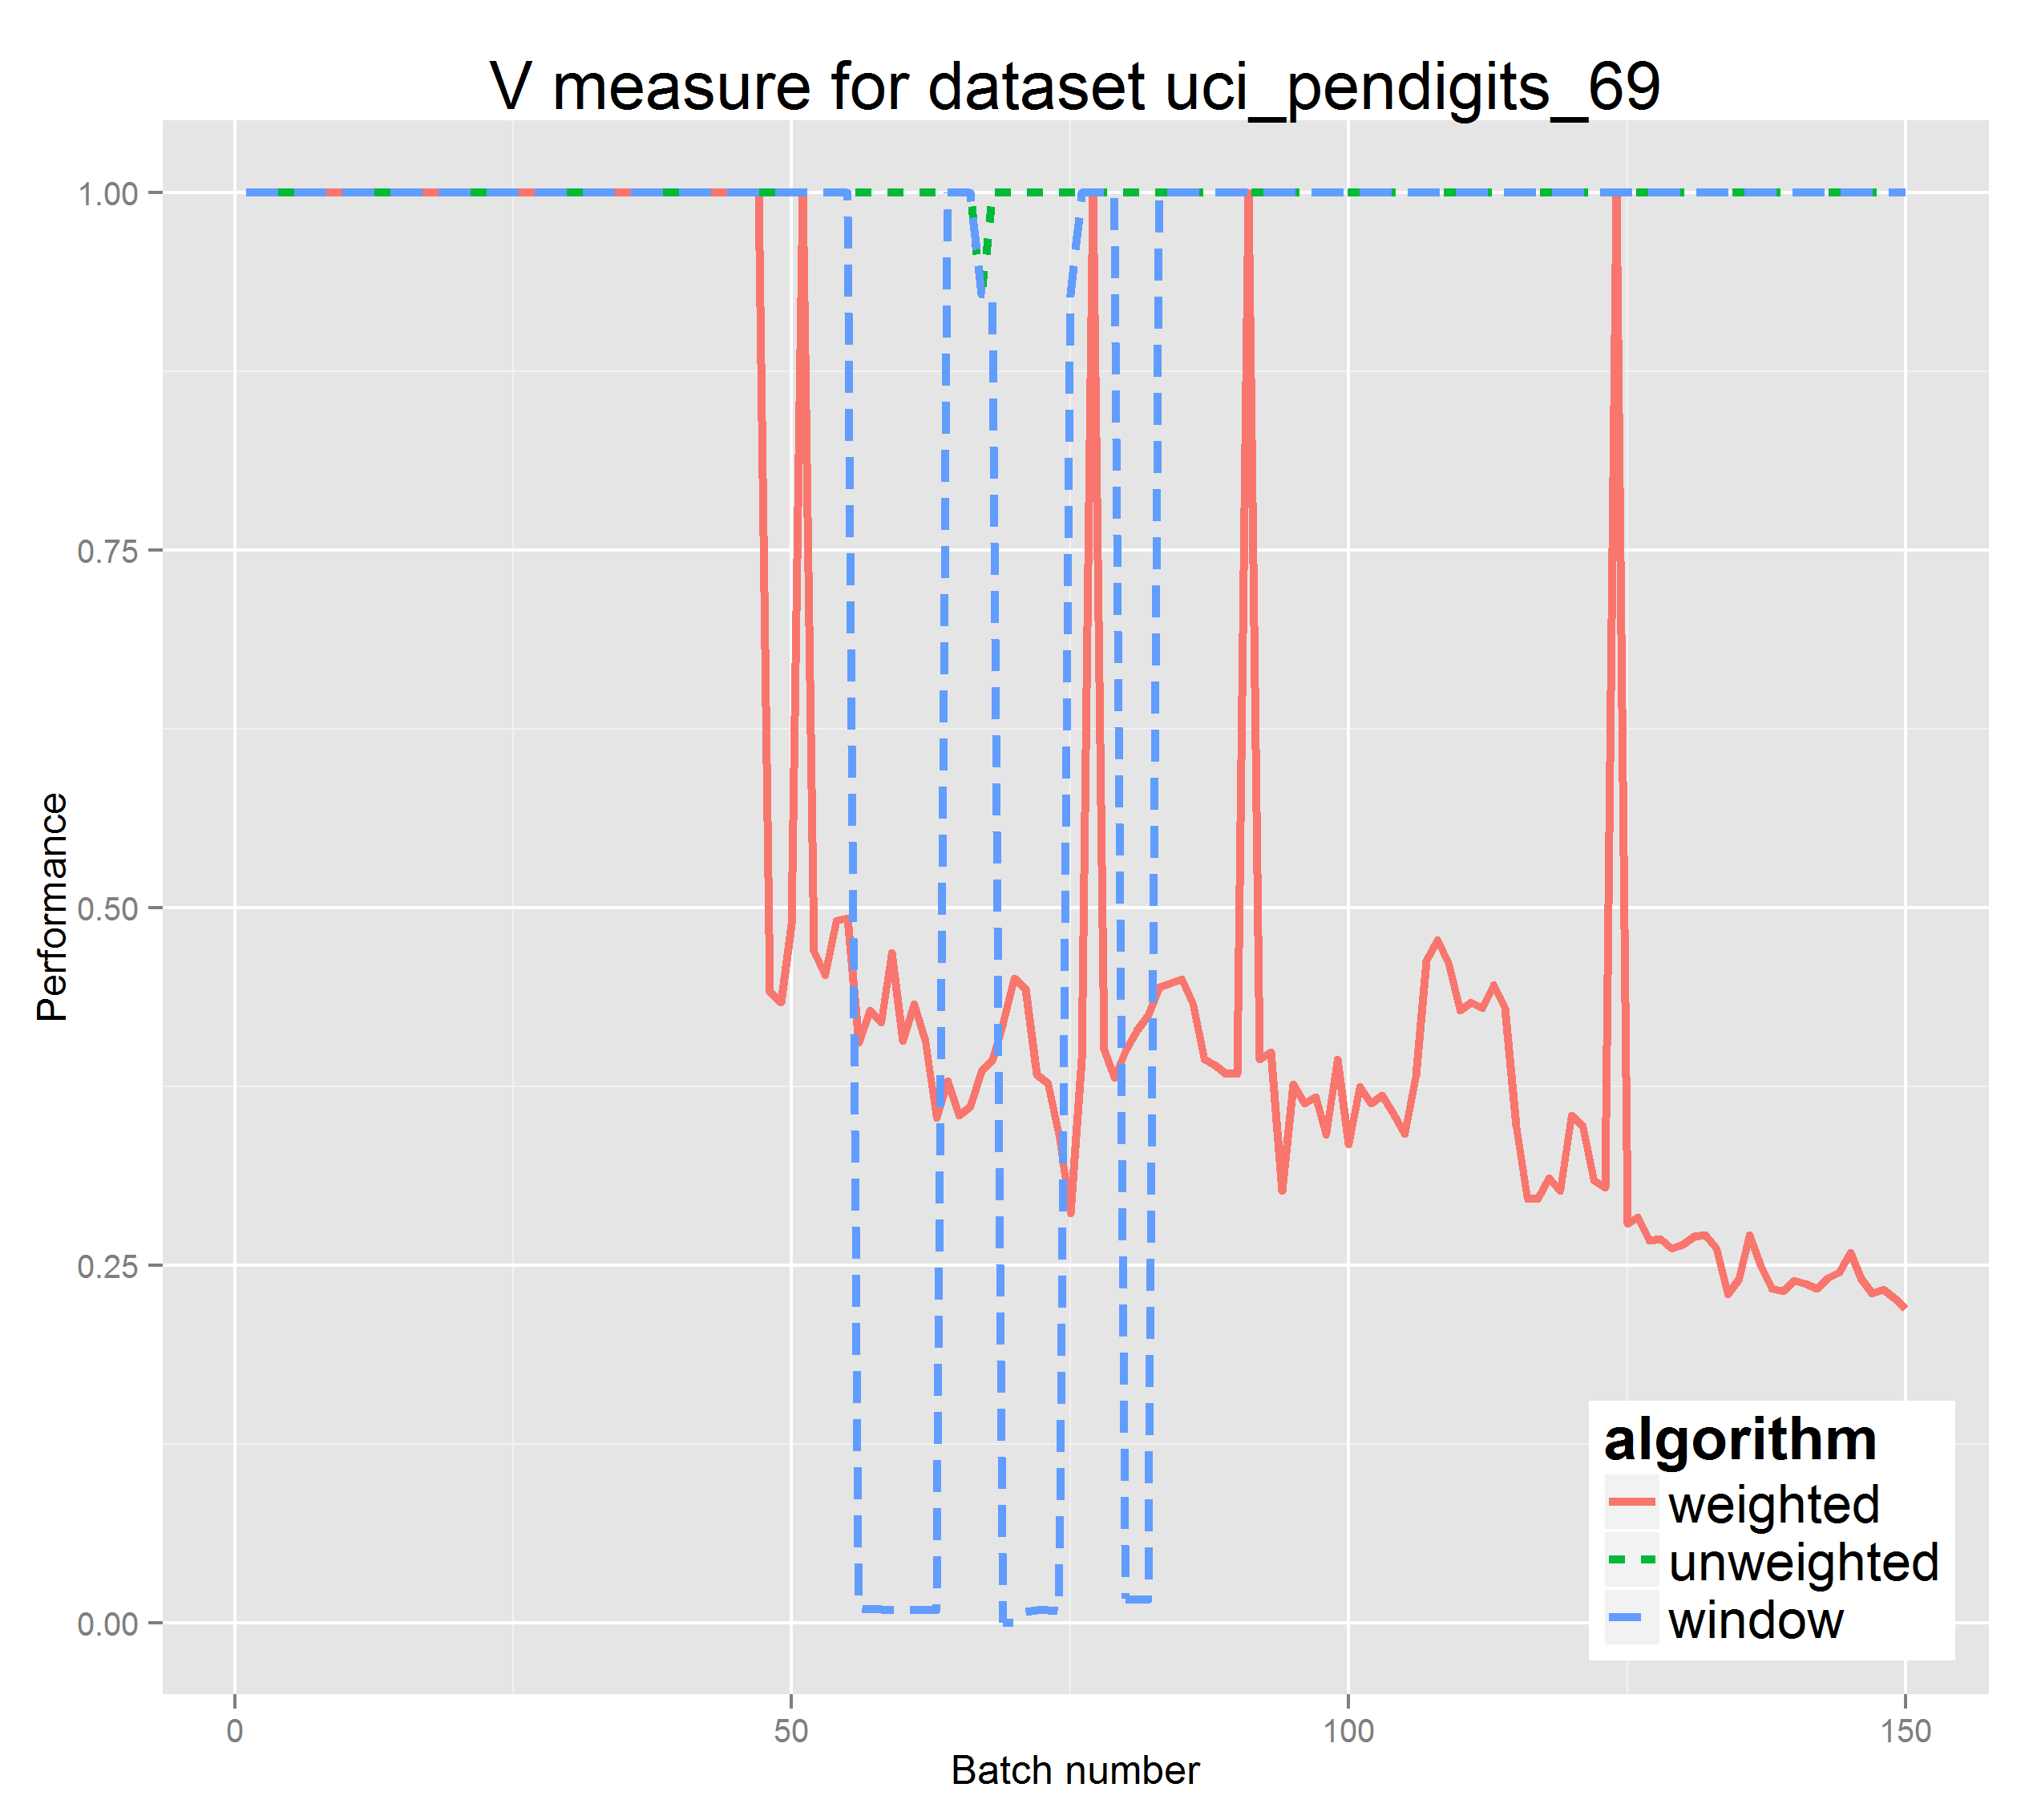
\includegraphics[width=.8\linewidth]{pendigit_results_2016_08_16/uci_pendigits_69_vmeasure.png}
  \caption{V-measure digits 6 and 9}
%  \label{fig:sfig2}
\end{subfigure}

\begin{subfigure}{.3\textwidth}
  \centering
  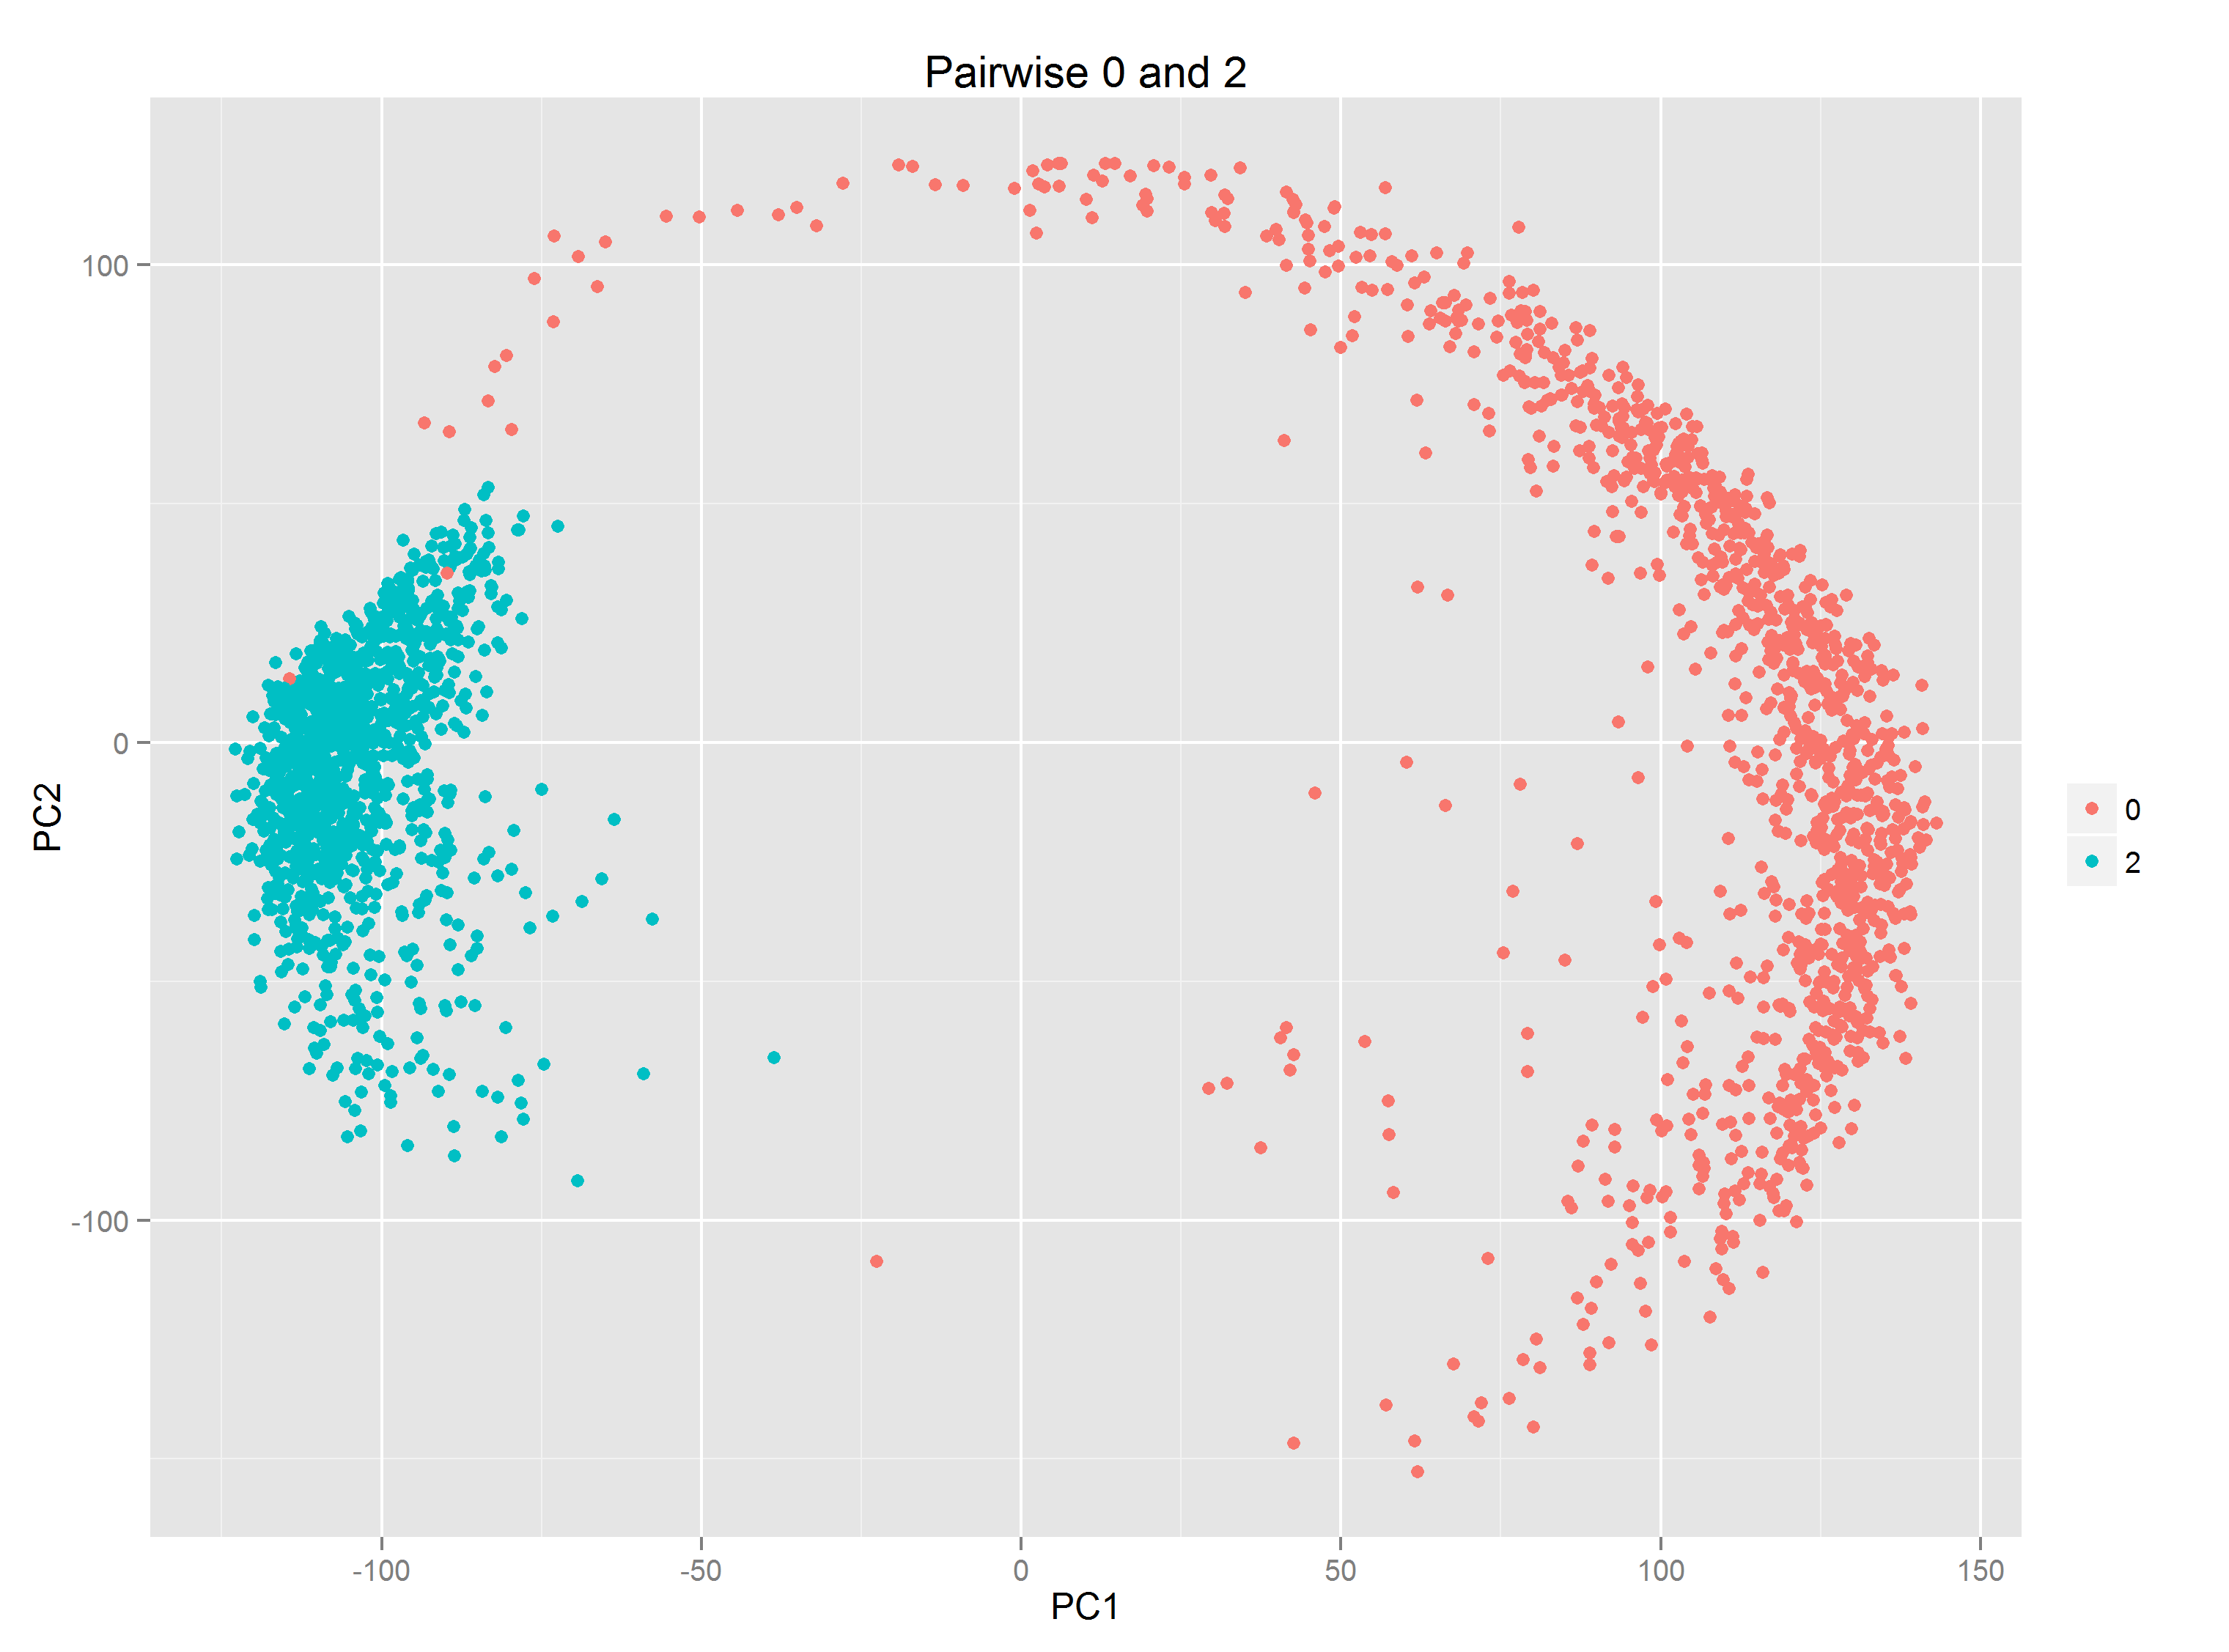
\includegraphics[width=.8\linewidth]{PCA_pendigits_pairwise/pairwise_0_2.png}
  \caption{PCA of digits 0 and 2}
 % \label{fig:sfig1}
\end{subfigure}%
\begin{subfigure}{.3\textwidth}
  \centering
  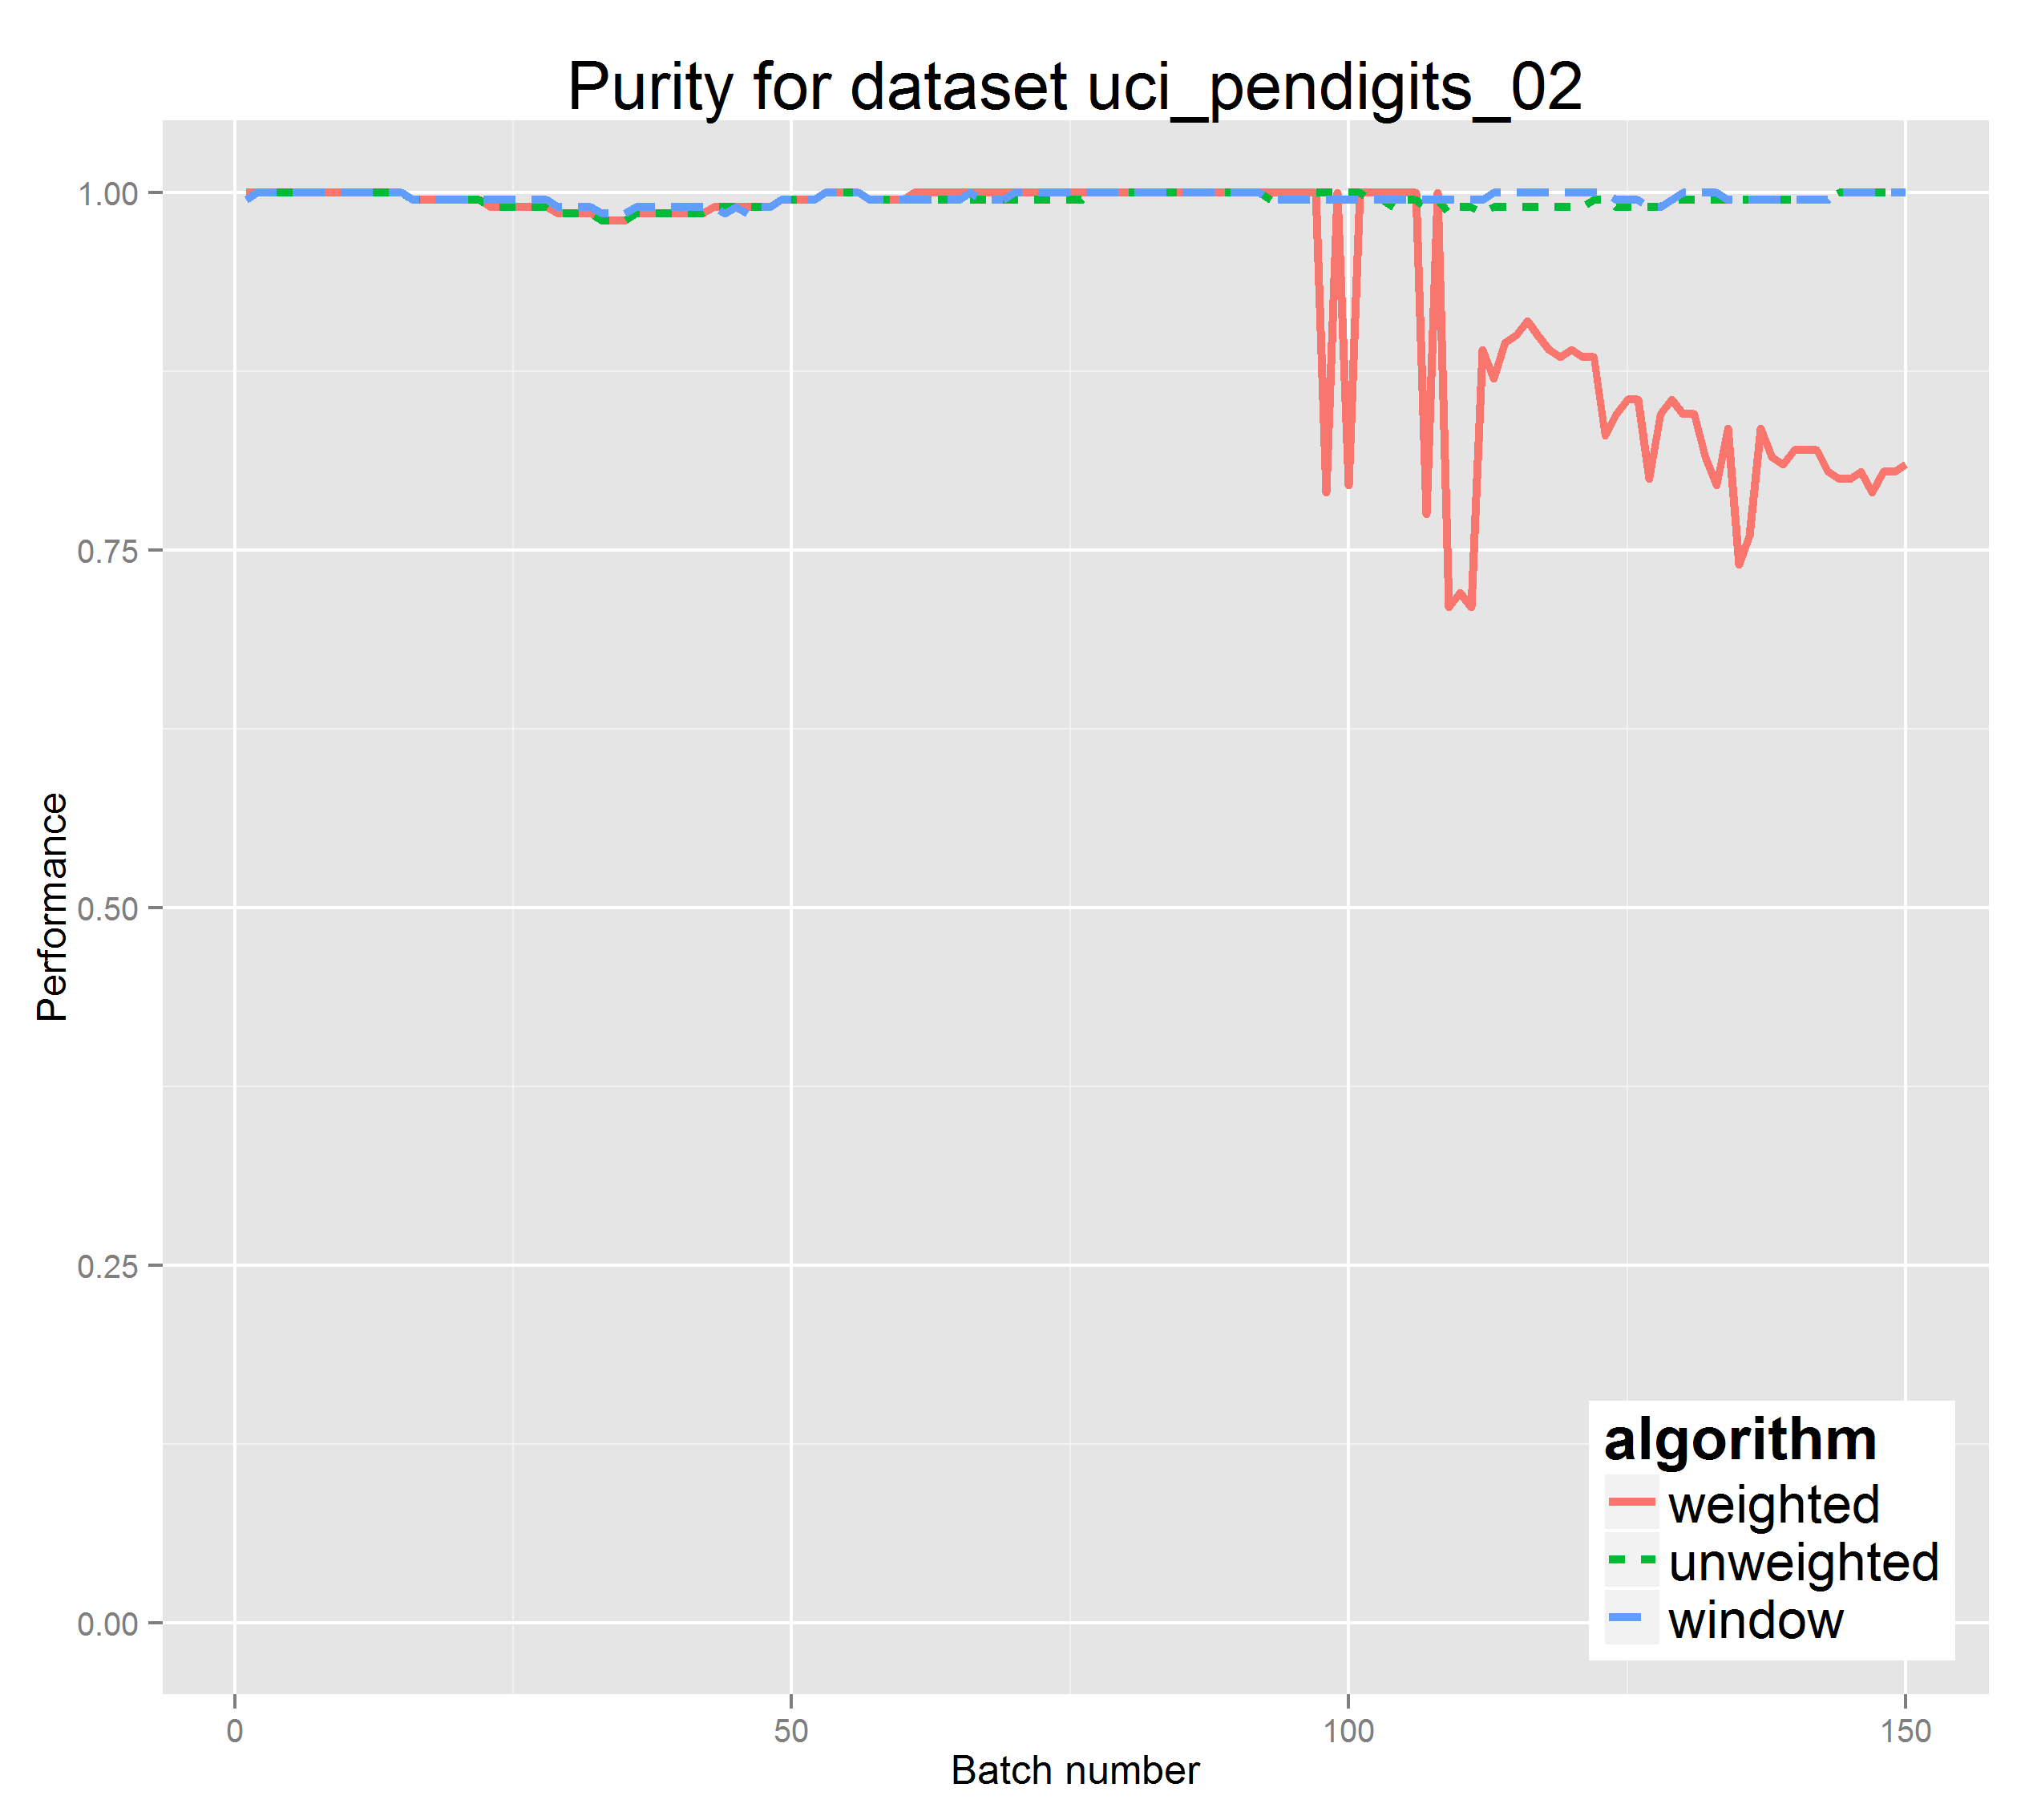
\includegraphics[width=.8\linewidth]{pendigit_results_2016_08_16/uci_pendigits_02_purity.png}
  \caption{Purity digits 0 and 2}
%  \label{fig:sfig2}
\end{subfigure}
\begin{subfigure}{.3\textwidth}
  \centering
  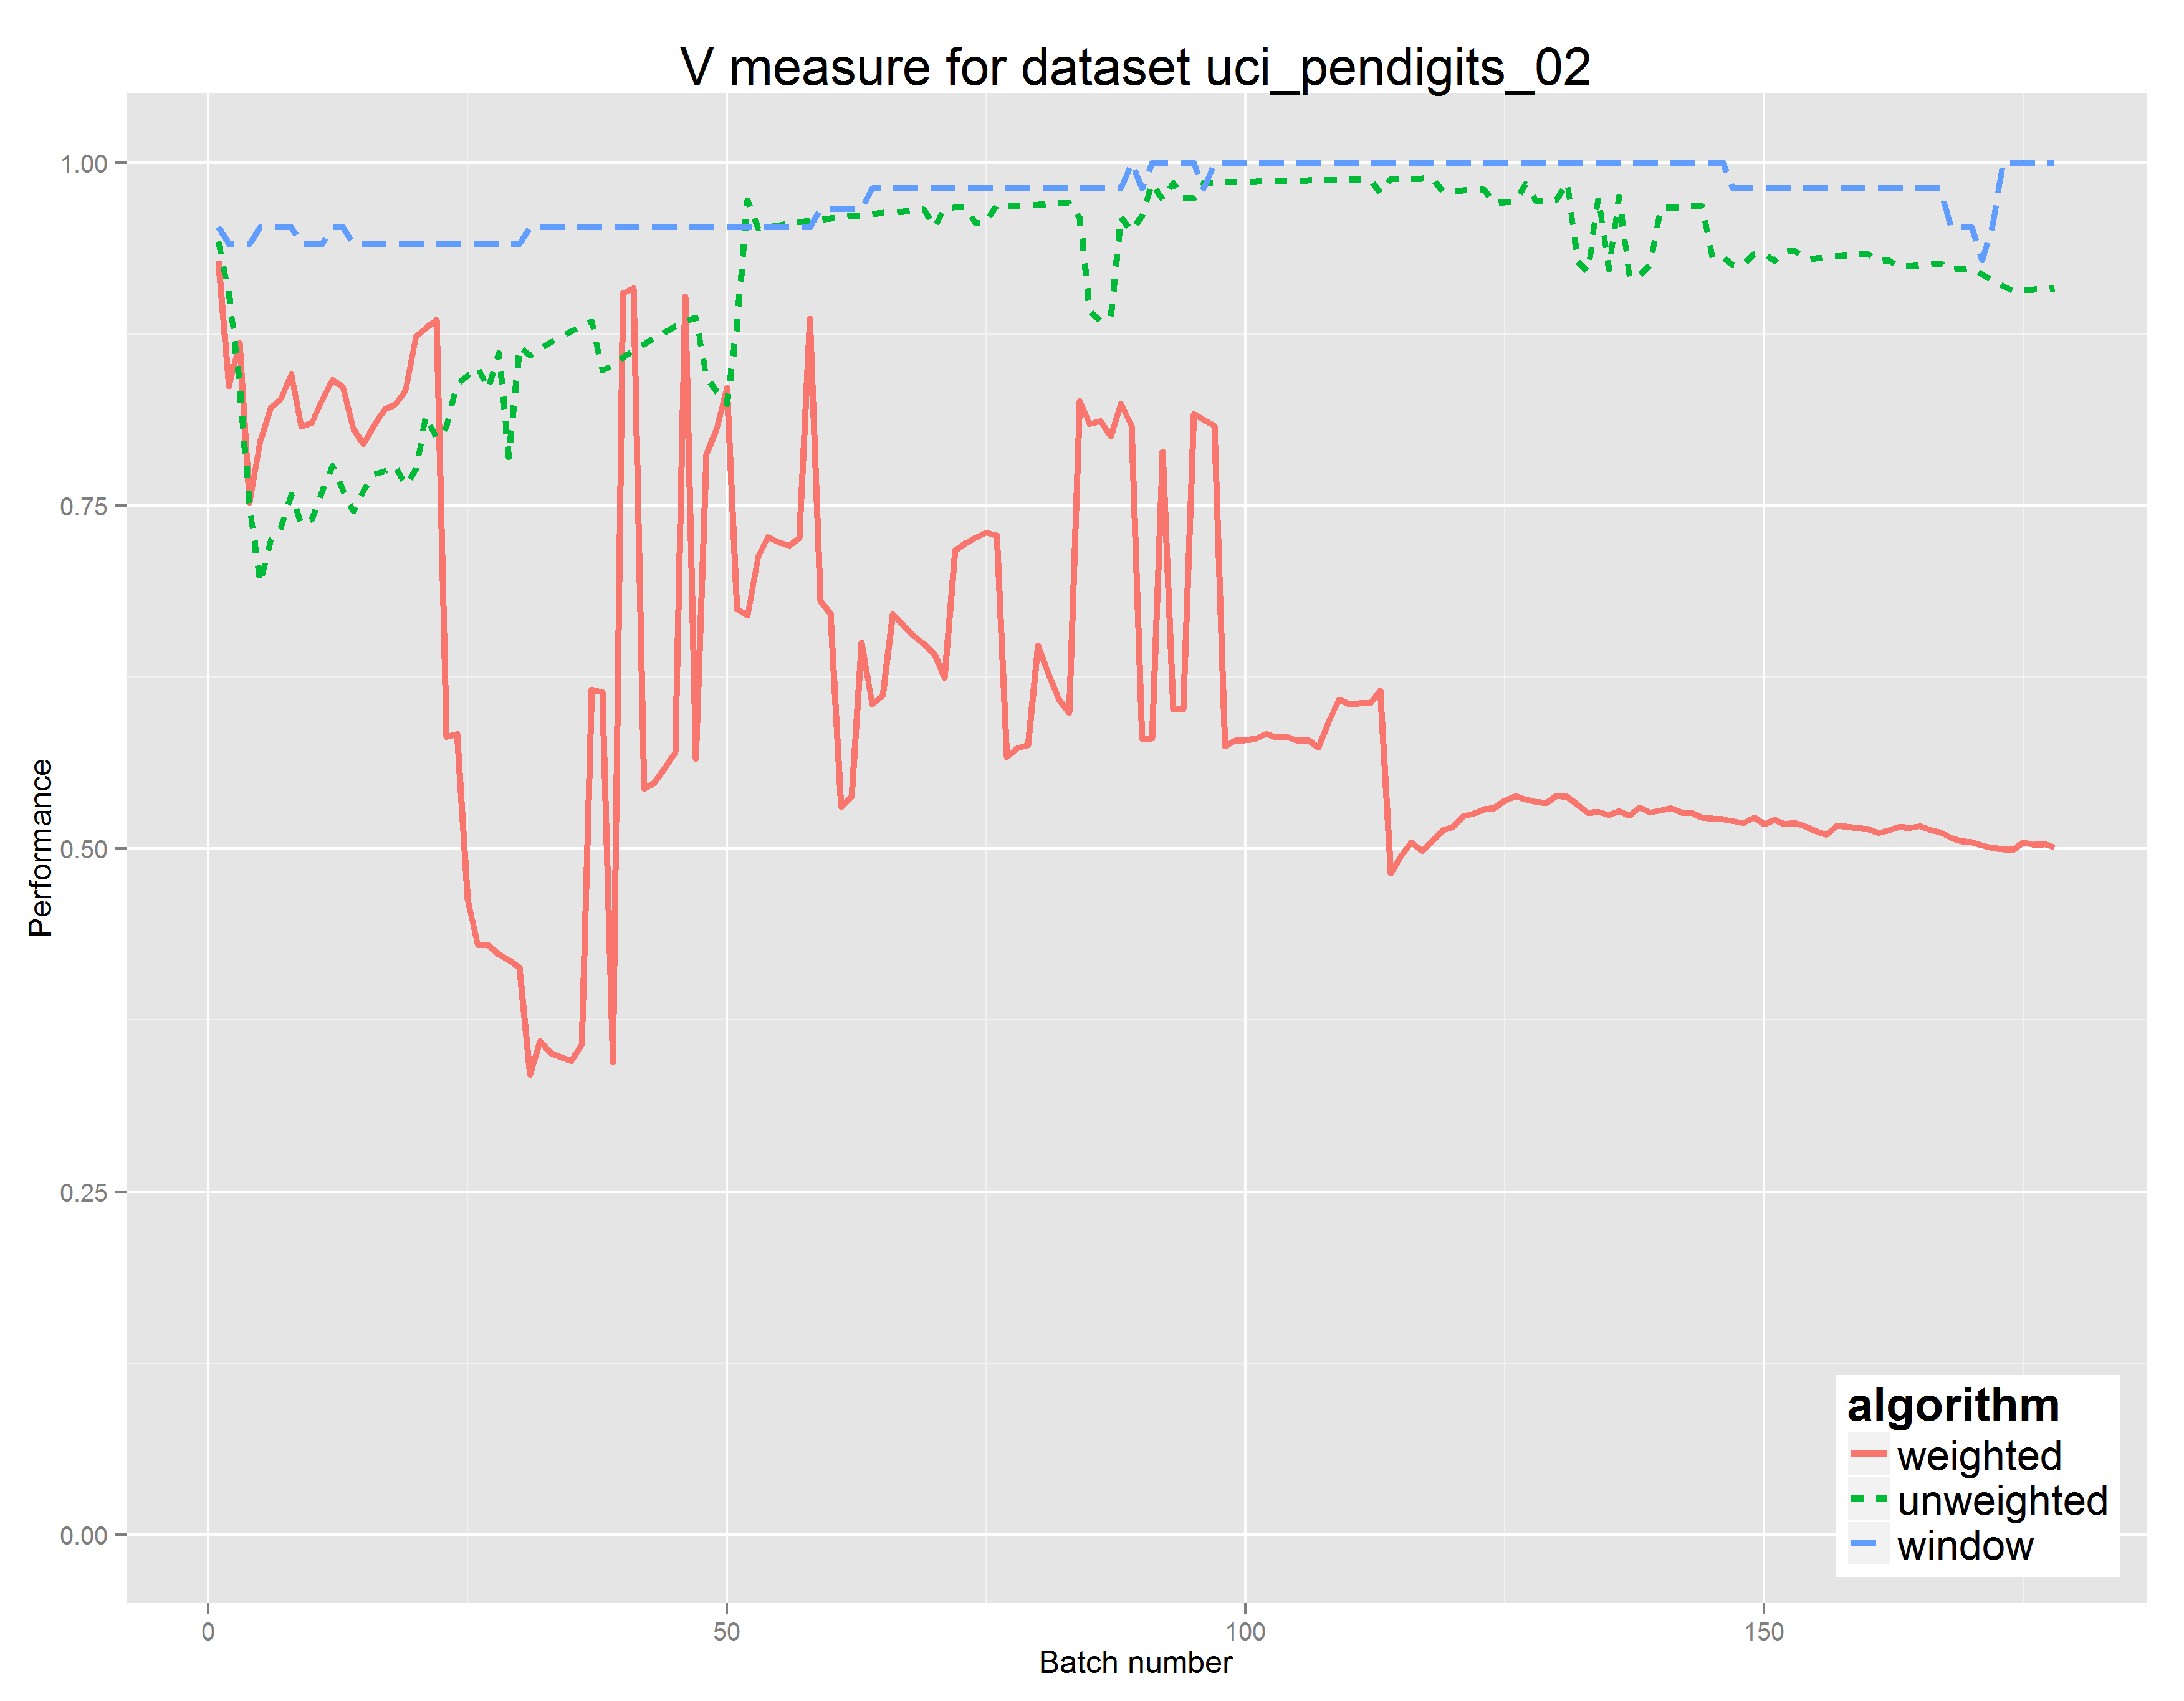
\includegraphics[width=.8\linewidth]{pendigit_results_2016_08_16/uci_pendigits_02_vmeasure.png}
  \caption{V-measure digits 0 and 2}
%  \label{fig:sfig2}
\end{subfigure}

\begin{subfigure}{.3\textwidth}
  \centering
  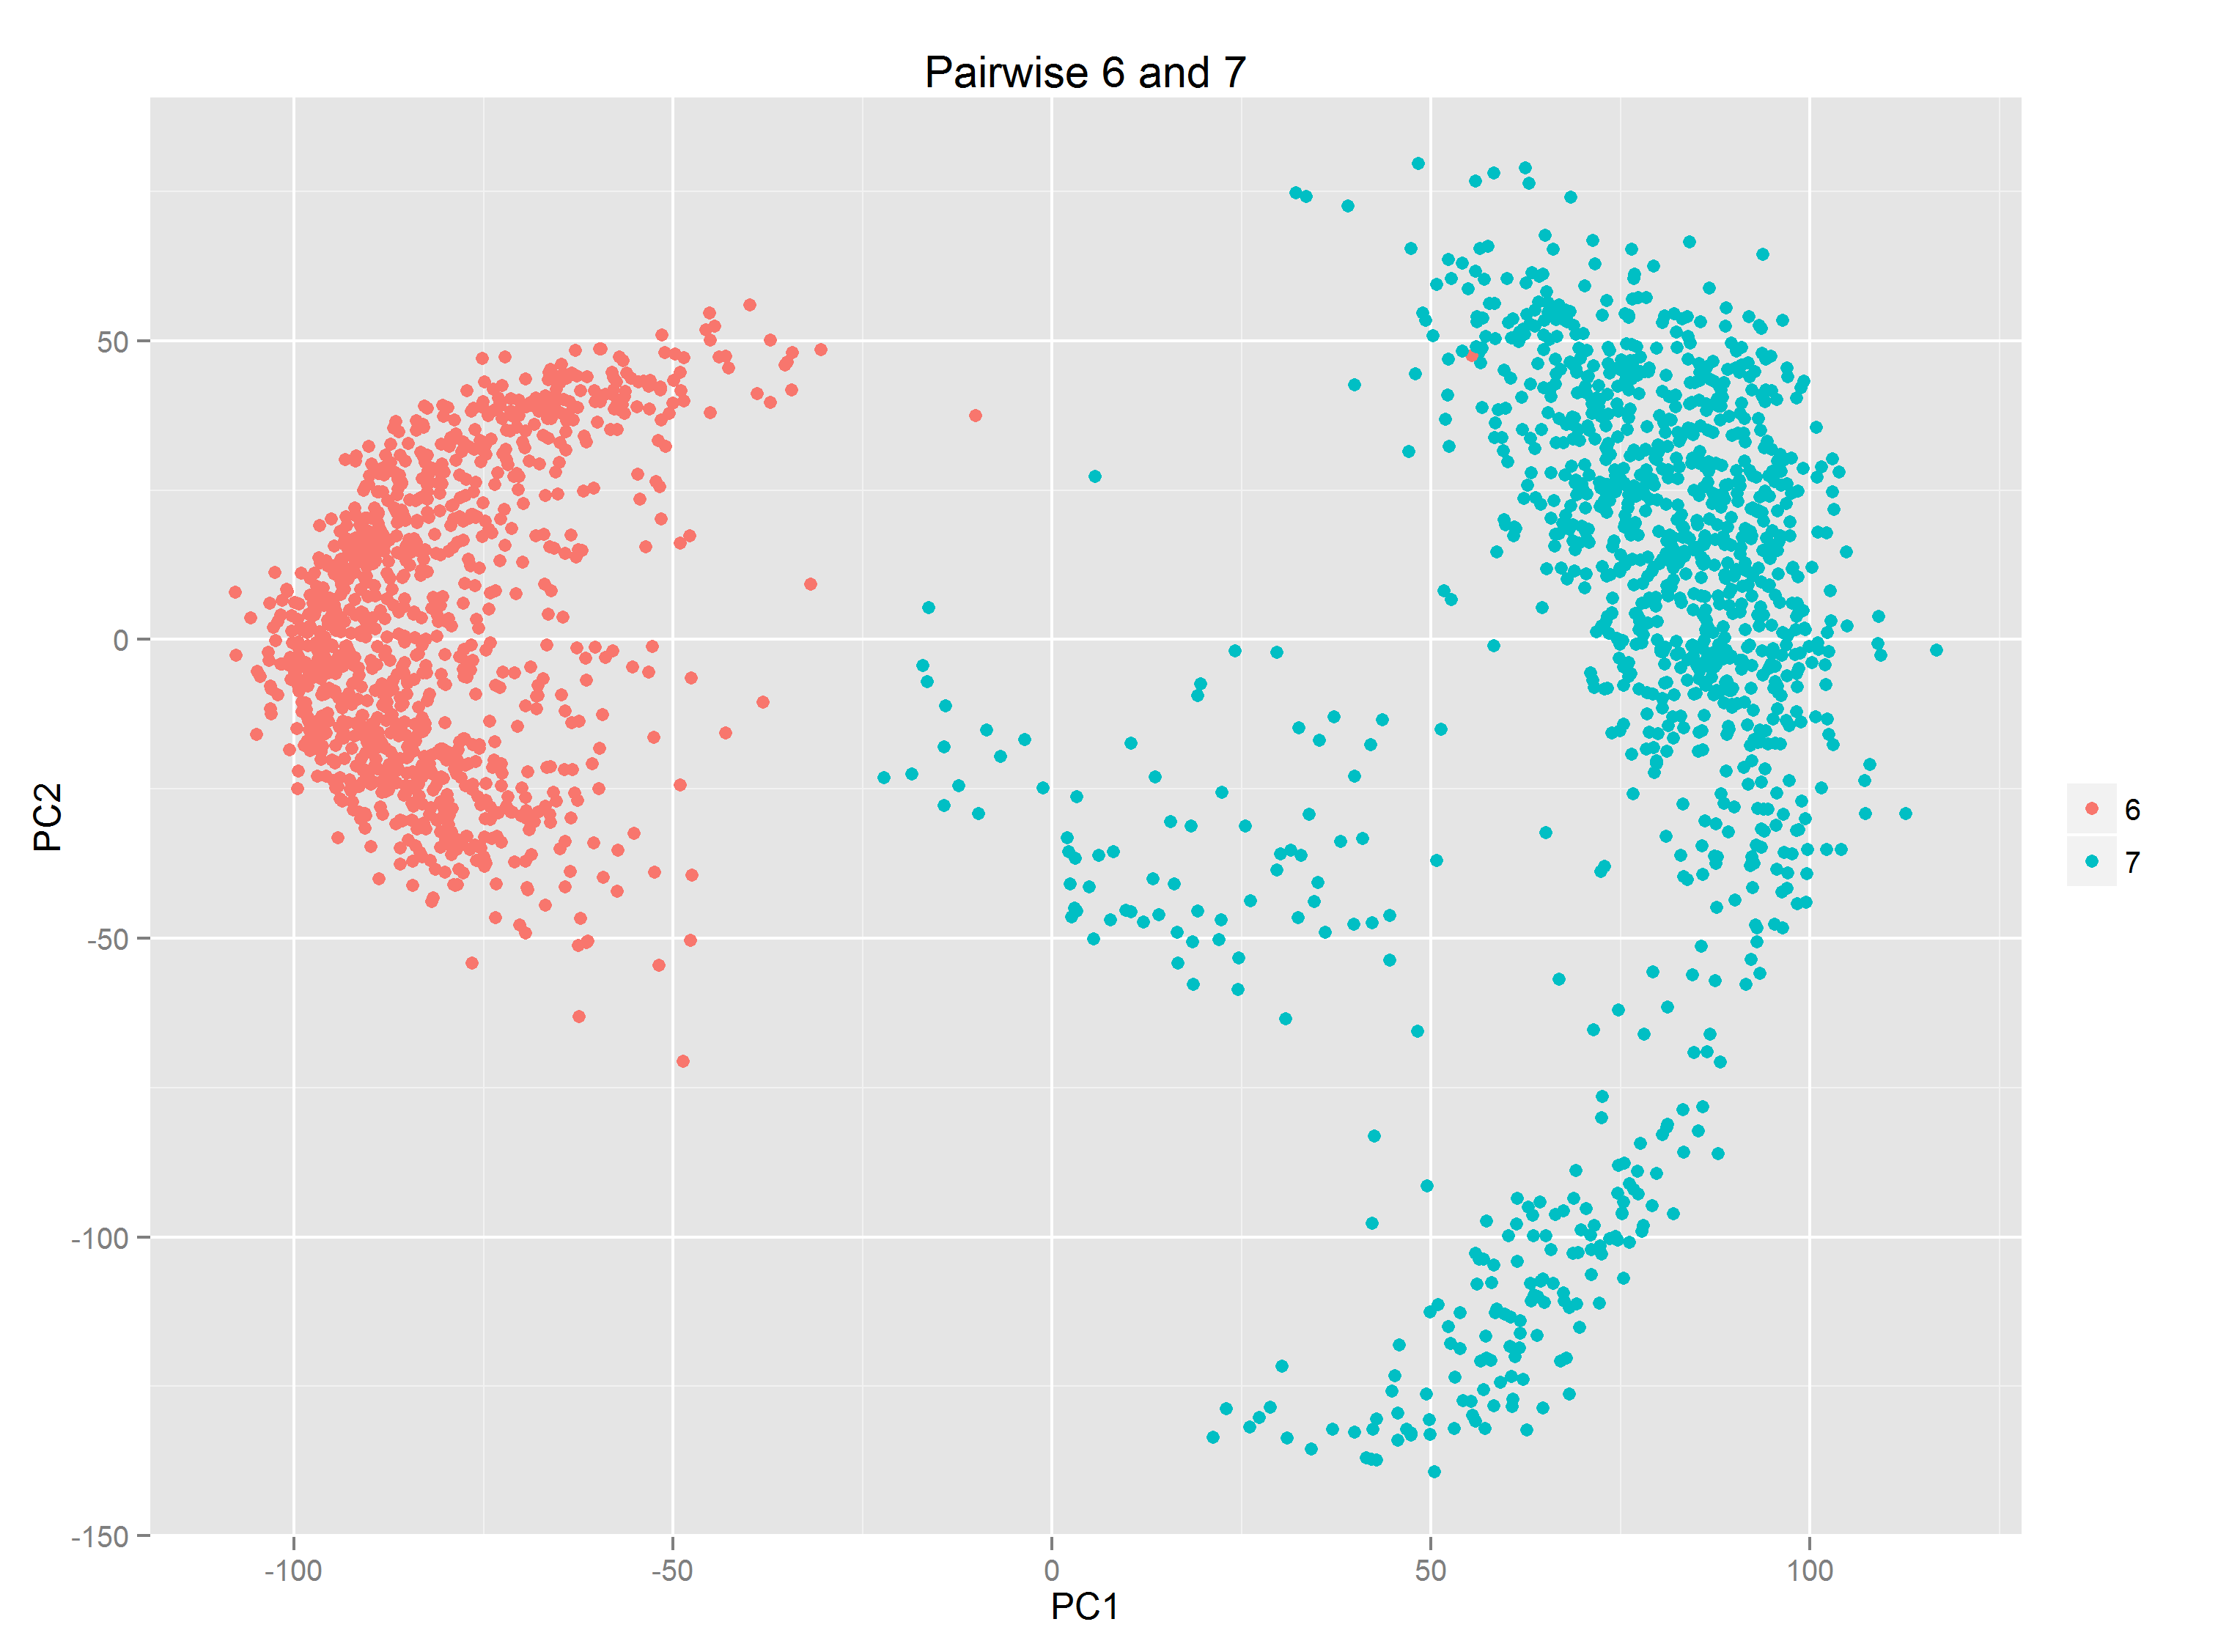
\includegraphics[width=.8\linewidth]{PCA_pendigits_pairwise/pairwise_6_7.png}
  \caption{PCA of digits 6 and 7}
 % \label{fig:sfig1}
\end{subfigure}%
\begin{subfigure}{.3\textwidth}
  \centering
  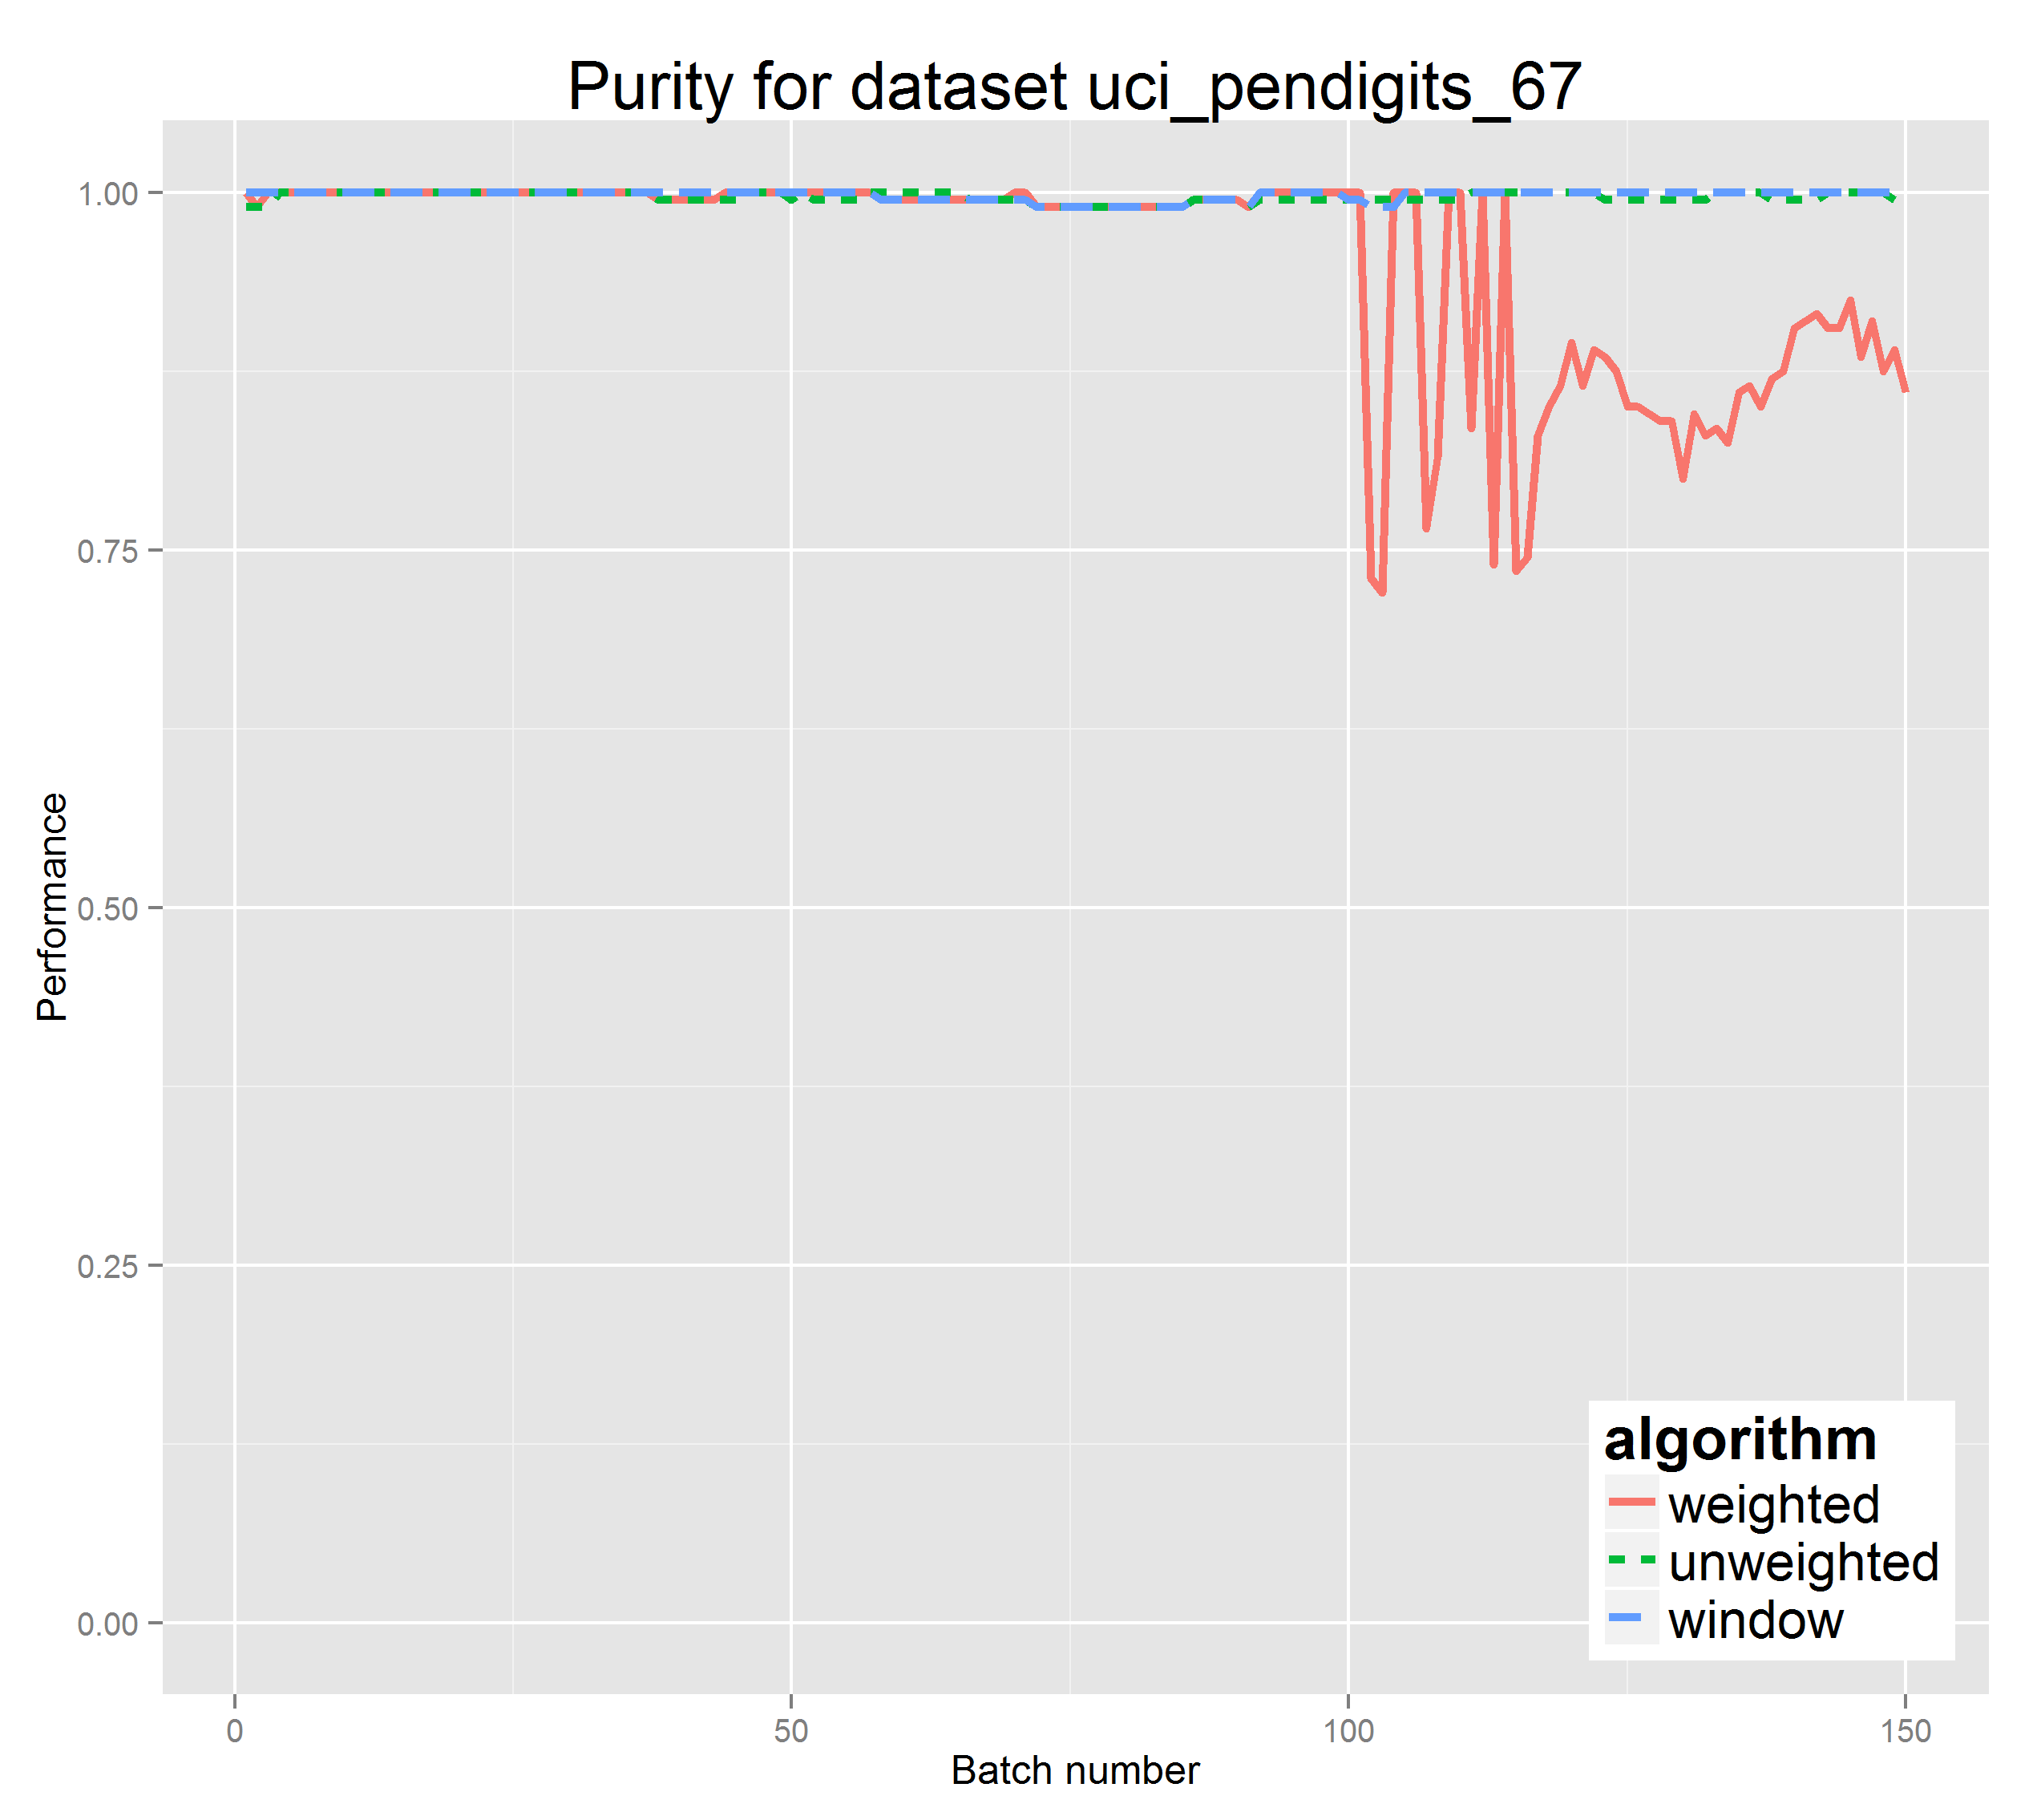
\includegraphics[width=.8\linewidth]{pendigit_results_2016_08_16/uci_pendigits_67_purity.png}
  \caption{Purity digits 6 and 7}
%  \label{fig:sfig2}
\end{subfigure}
\begin{subfigure}{.3\textwidth}
  \centering
  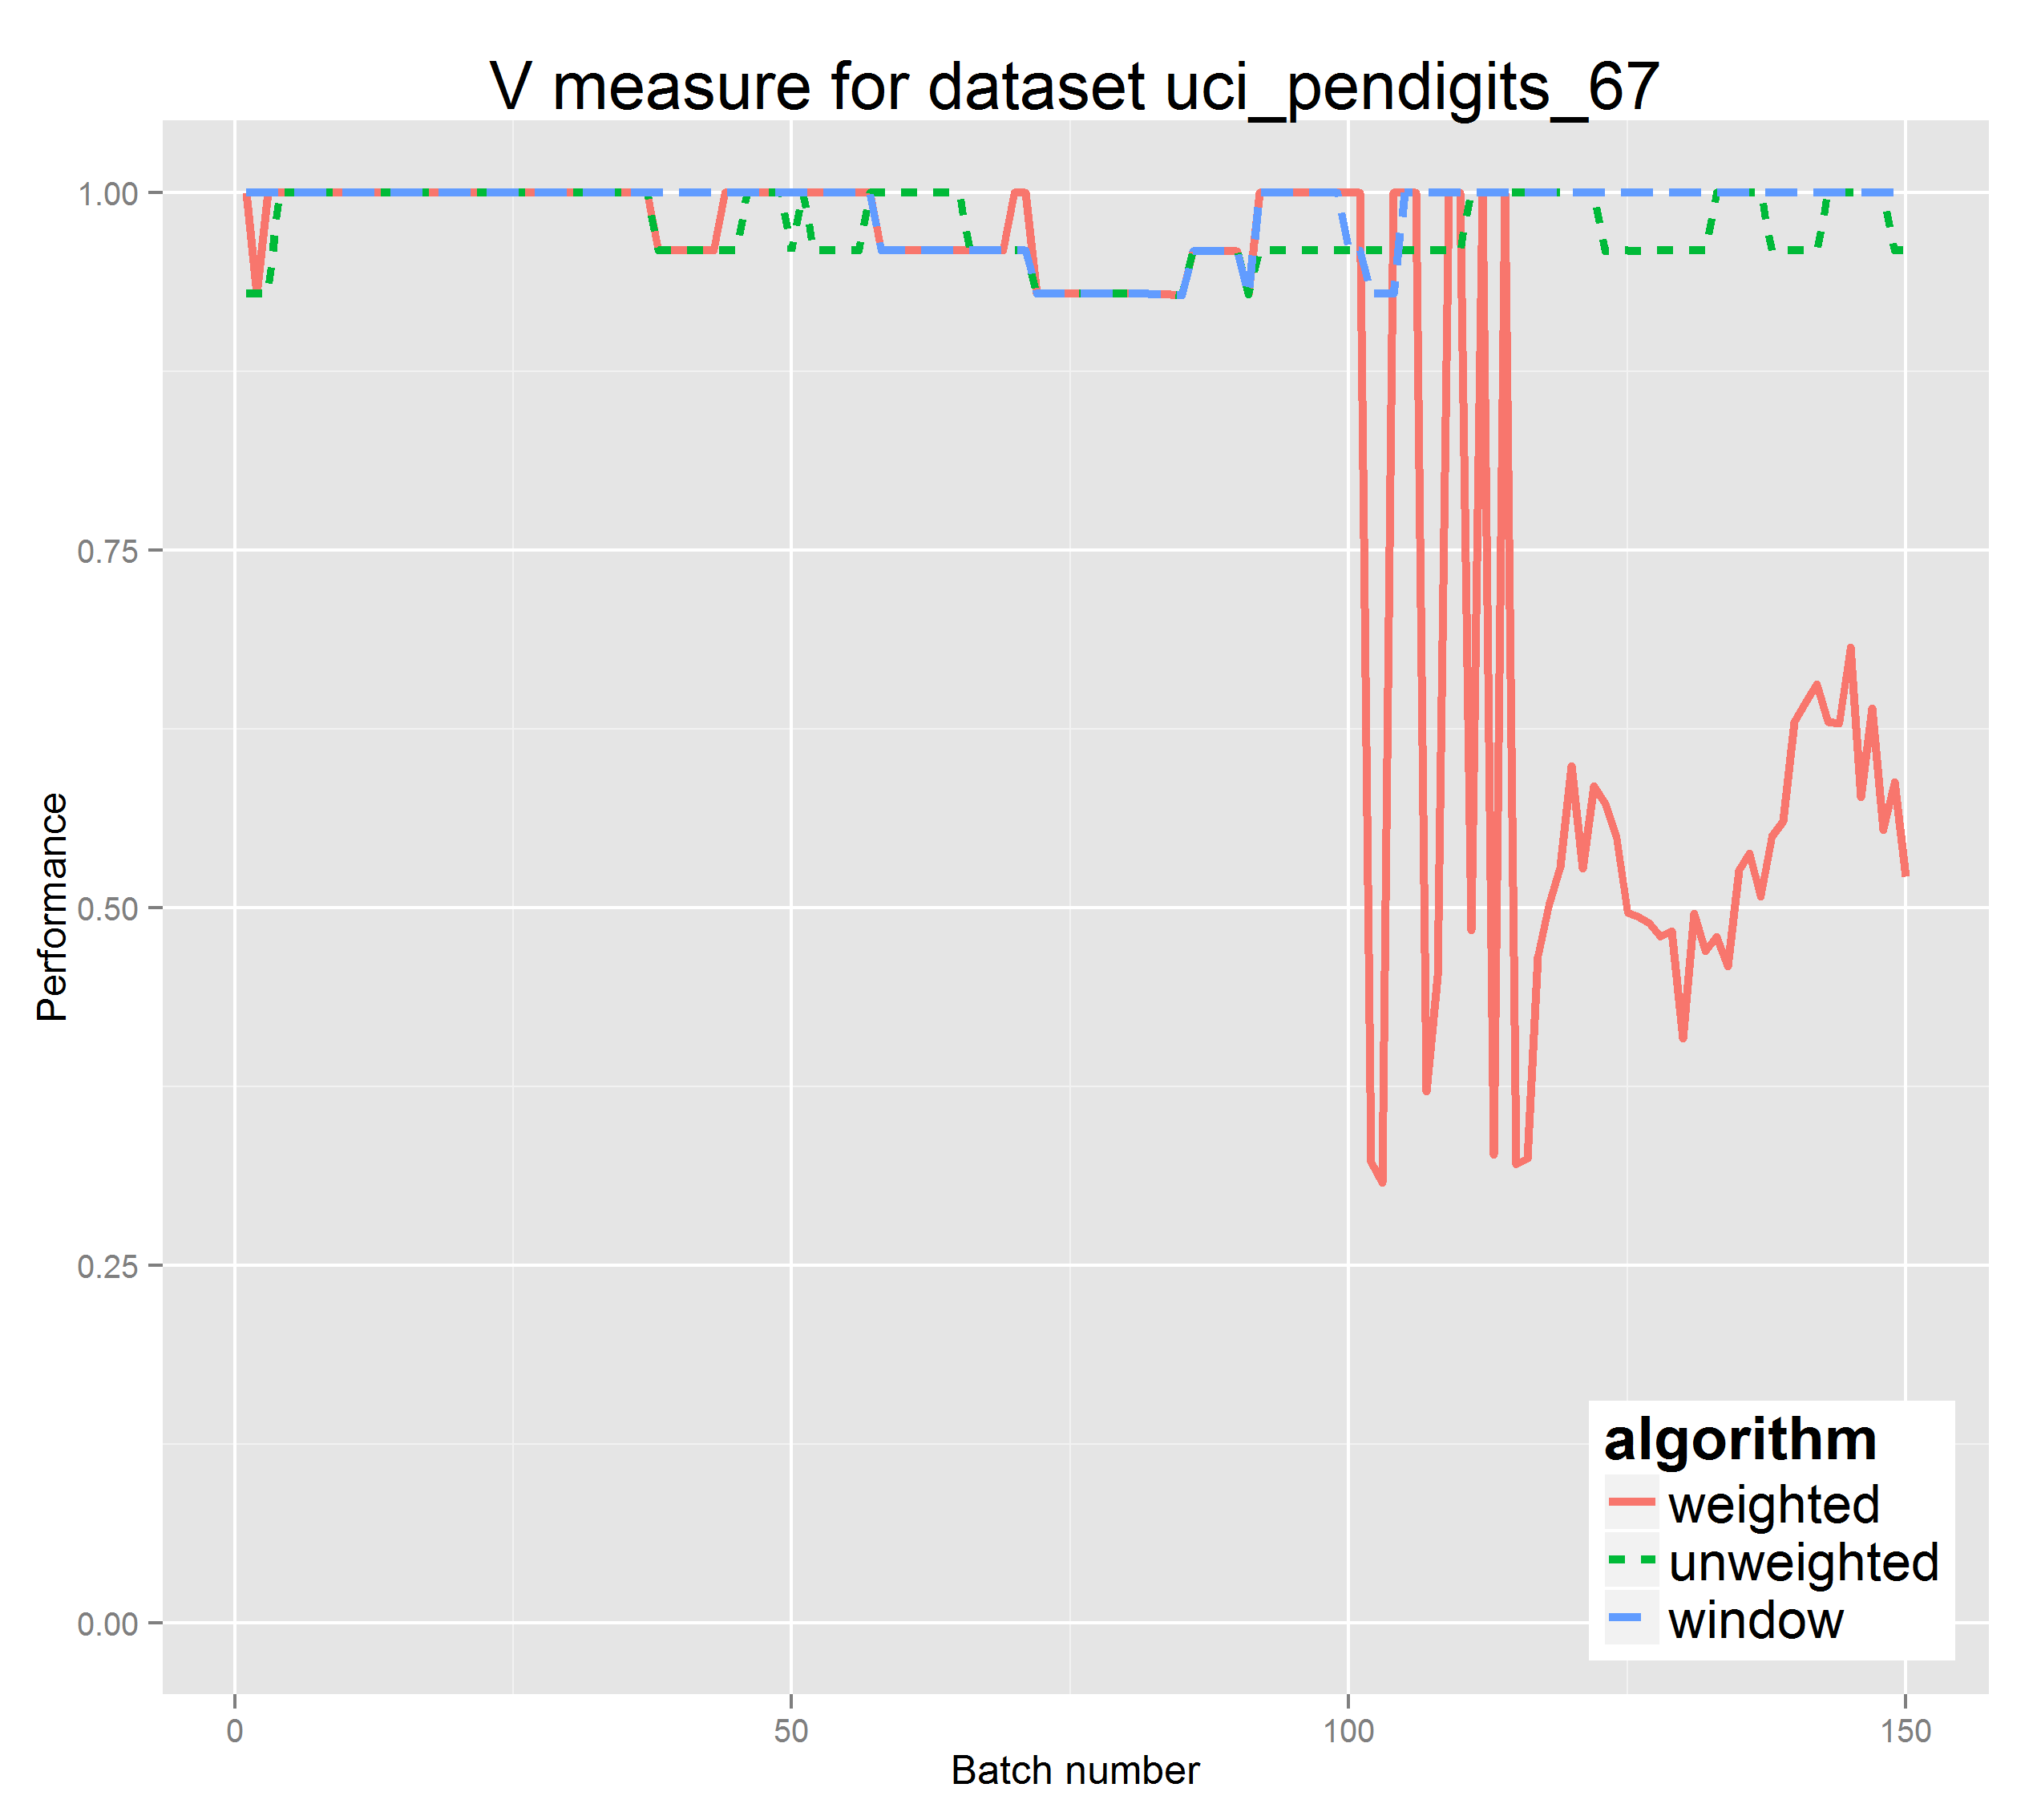
\includegraphics[width=.8\linewidth]{pendigit_results_2016_08_16/uci_pendigits_67_vmeasure.png}
  \caption{V-measure digits 6 and 7}
%  \label{fig:sfig2}
\end{subfigure}

\caption{Pendigits Pairwise - Clustream and windowed spectral}
\label{fig:uci_pendigits}
\end{figure}


\subsubsection{Texture data}

We also tested there methods on another set of real data based on textured images. The Kylberg \citep{kylberg2011c} texture data set consists of 28 texture classes with 160 unique texture patches per class. The patches consist of $576 \times 576$ pixel images.

In order to extract features to cluster, I used the LS2W \citep{Eckley2011} method to extract wavelet features of from the textured images.

I selected a subset of 6 classes to run the algorithms on, examples of all 6 textures are shown in Figure \ref{fig:texture_examples} .  The classes selected represent, two types of blanket, canvas, a ceiling, some lentils and a screen.

\begin{figure}[h!]
\begin{subfigure}{.15\textwidth}
  \centering
  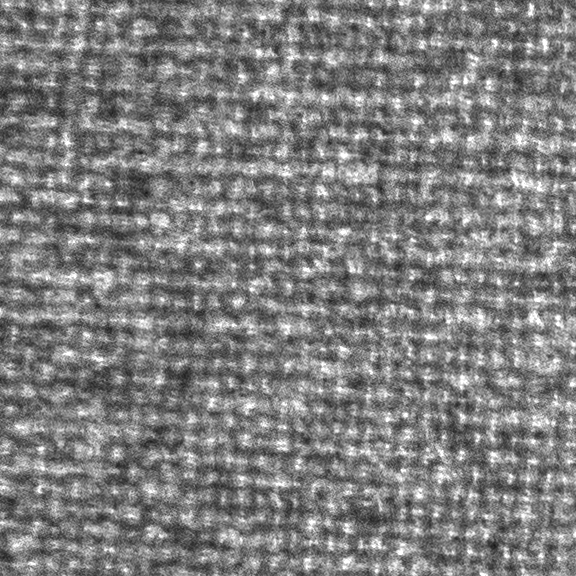
\includegraphics[width=.8\linewidth]{kylberg_examples/blanket1_001.png}
  %\caption{PCA of digits 2 and 9}
 % \label{fig:sfig1}
\end{subfigure}%
\begin{subfigure}{.15\textwidth}
  \centering
  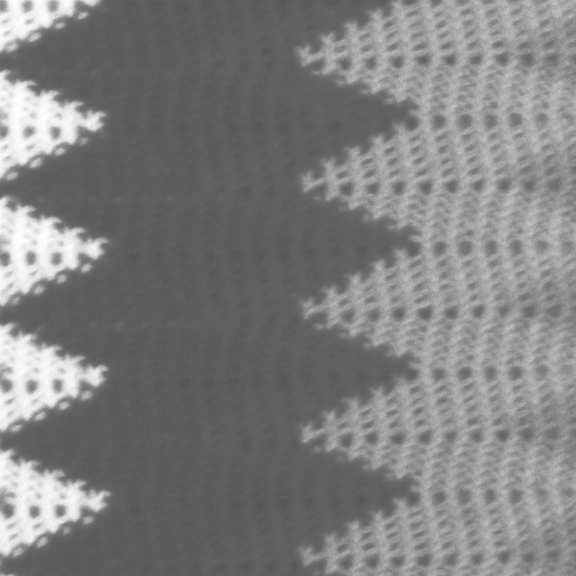
\includegraphics[width=.8\linewidth]{kylberg_examples/blanket2_001.png}
  %\caption{Purity digits 2 and 9}
%  \label{fig:sfig2}
\end{subfigure}
\begin{subfigure}{.15\textwidth}
  \centering
  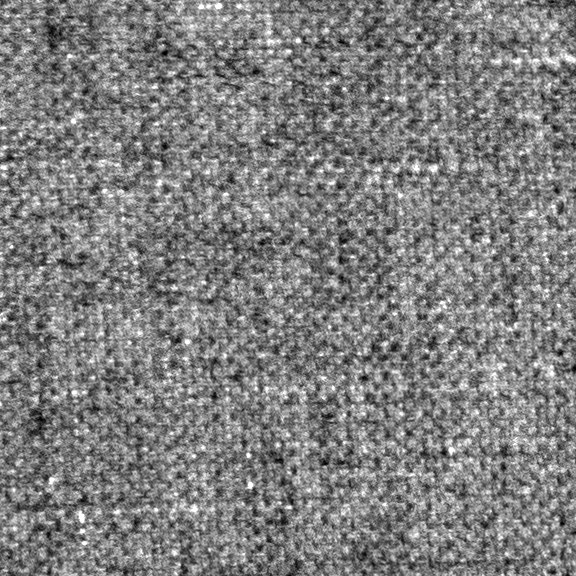
\includegraphics[width=.8\linewidth]{kylberg_examples/canvas1_001.png}
  %\caption{V-measure digits 2 and 9}
%  \label{fig:sfig2}
\end{subfigure}
\begin{subfigure}{.15\textwidth}
  \centering
  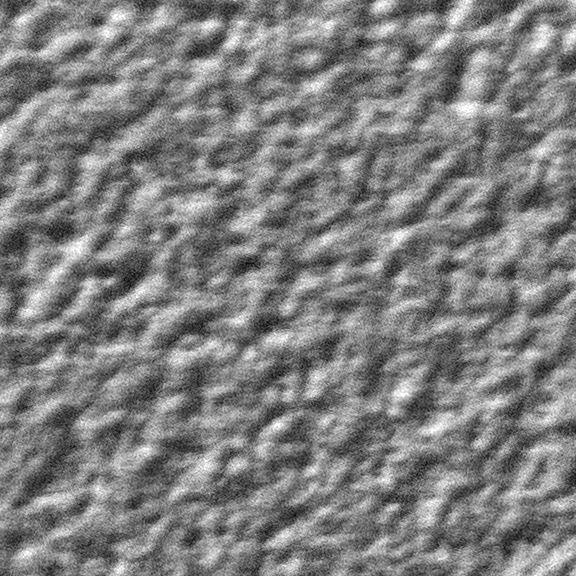
\includegraphics[width=.8\linewidth]{kylberg_examples/ceiling1_001.png}
  %\caption{PCA of digits 2 and 9}
 % \label{fig:sfig1}
\end{subfigure}%
\begin{subfigure}{.15\textwidth}
  \centering
  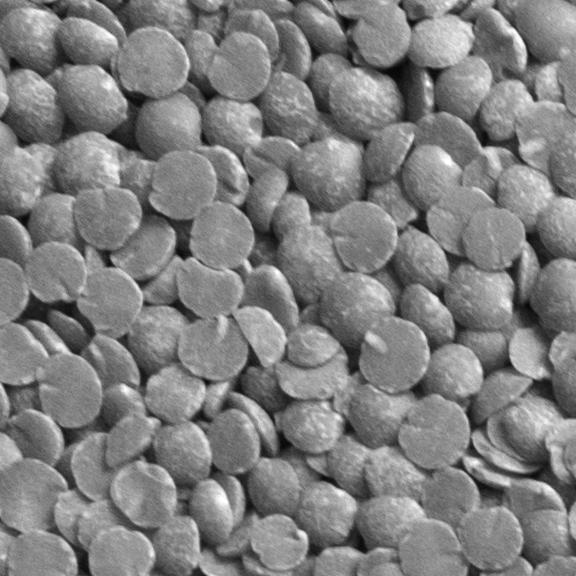
\includegraphics[width=.8\linewidth]{kylberg_examples/lentils1_001.png}
  %\caption{Purity digits 2 and 9}
%  \label{fig:sfig2}
\end{subfigure}
\begin{subfigure}{.15\textwidth}
  \centering
  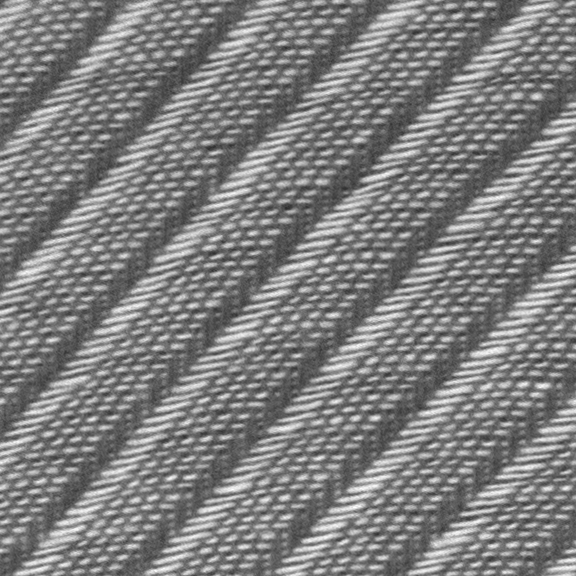
\includegraphics[width=.8\linewidth]{kylberg_examples/screen1_001.png}
  %\caption{V-measure digits 2 and 9}
%  \label{fig:sfig2}
\end{subfigure}

\begin{subfigure}{.15\textwidth}
  \centering
  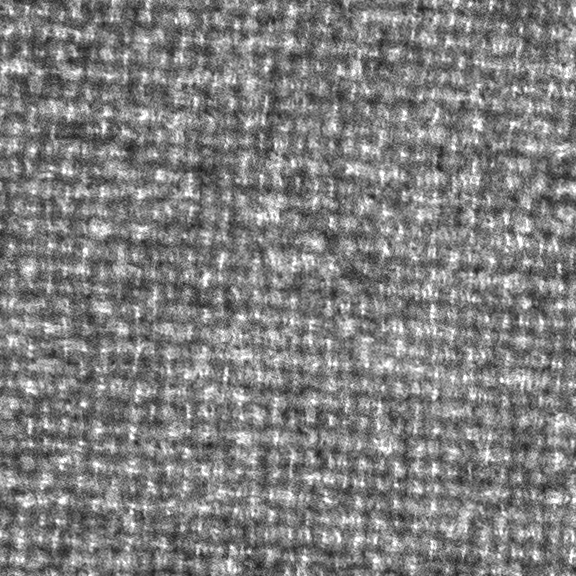
\includegraphics[width=.8\linewidth]{kylberg_examples/blanket1_002.png}
  %\caption{PCA of digits 2 and 9}
 % \label{fig:sfig1}
\end{subfigure}%
\begin{subfigure}{.15\textwidth}
  \centering
  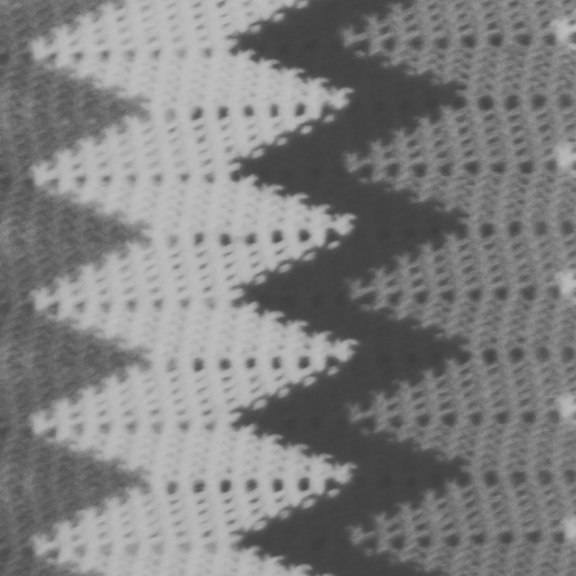
\includegraphics[width=.8\linewidth]{kylberg_examples/blanket2_002.png}
  %\caption{Purity digits 2 and 9}
%  \label{fig:sfig2}
\end{subfigure}
\begin{subfigure}{.15\textwidth}
  \centering
  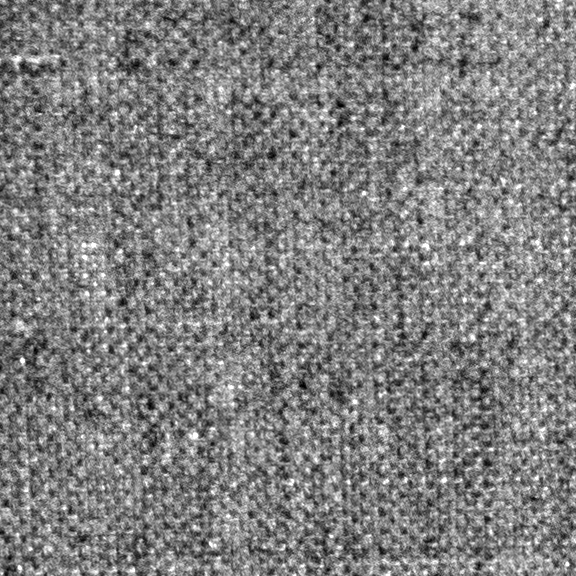
\includegraphics[width=.8\linewidth]{kylberg_examples/canvas1_002.png}
  %\caption{V-measure digits 2 and 9}
%  \label{fig:sfig2}
\end{subfigure}
\begin{subfigure}{.15\textwidth}
  \centering
  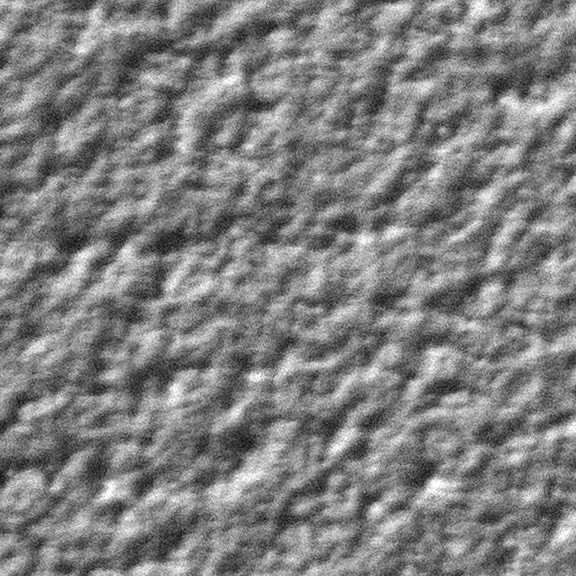
\includegraphics[width=.8\linewidth]{kylberg_examples/ceiling1_002.png}
  %\caption{PCA of digits 2 and 9}
 % \label{fig:sfig1}
\end{subfigure}%
\begin{subfigure}{.15\textwidth}
  \centering
  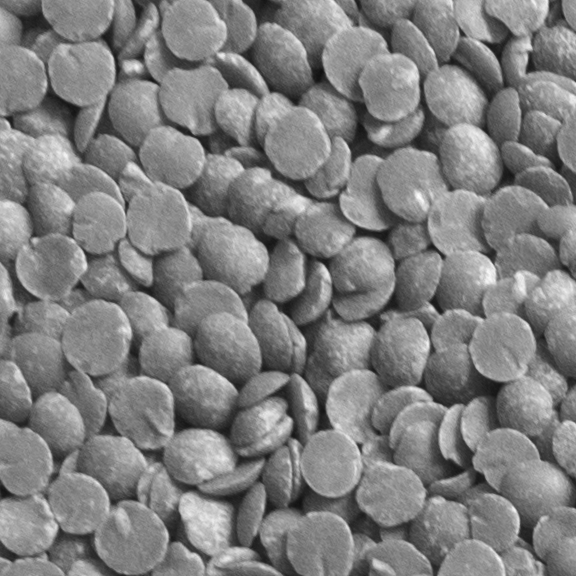
\includegraphics[width=.8\linewidth]{kylberg_examples/lentils1_002.png}
  %\caption{Purity digits 2 and 9}
%  \label{fig:sfig2}
\end{subfigure}
\begin{subfigure}{.15\textwidth}
  \centering
  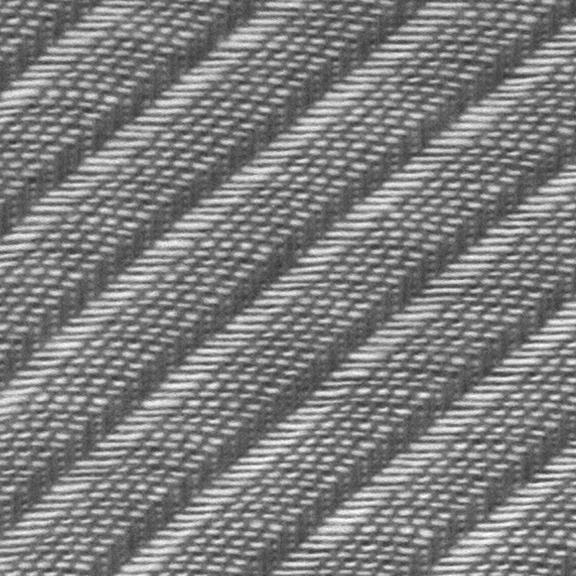
\includegraphics[width=.8\linewidth]{kylberg_examples/screen1_002.png}
  %\caption{V-measure digits 2 and 9}
%  \label{fig:sfig2}
\end{subfigure}

\begin{subfigure}{.15\textwidth}
  \centering
  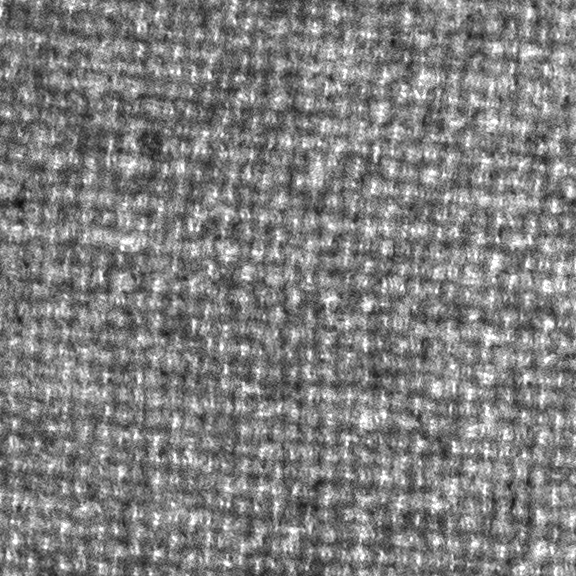
\includegraphics[width=.8\linewidth]{kylberg_examples/blanket1_003.png}
  %\caption{PCA of digits 2 and 9}
 % \label{fig:sfig1}
\end{subfigure}%
\begin{subfigure}{.15\textwidth}
  \centering
  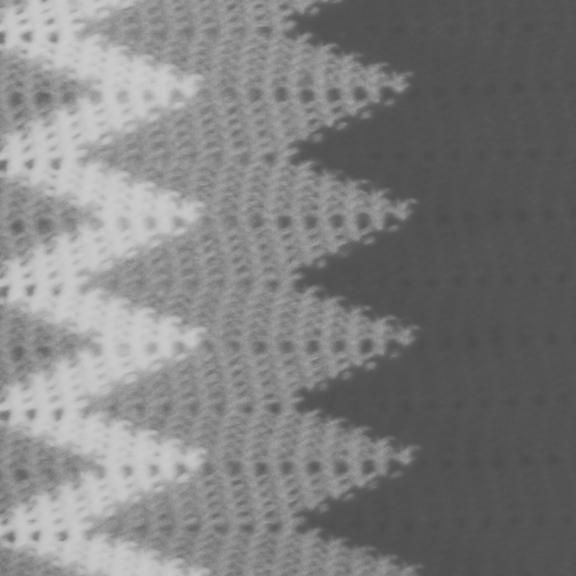
\includegraphics[width=.8\linewidth]{kylberg_examples/blanket2_003.png}
  %\caption{Purity digits 2 and 9}
%  \label{fig:sfig2}
\end{subfigure}
\begin{subfigure}{.15\textwidth}
  \centering
  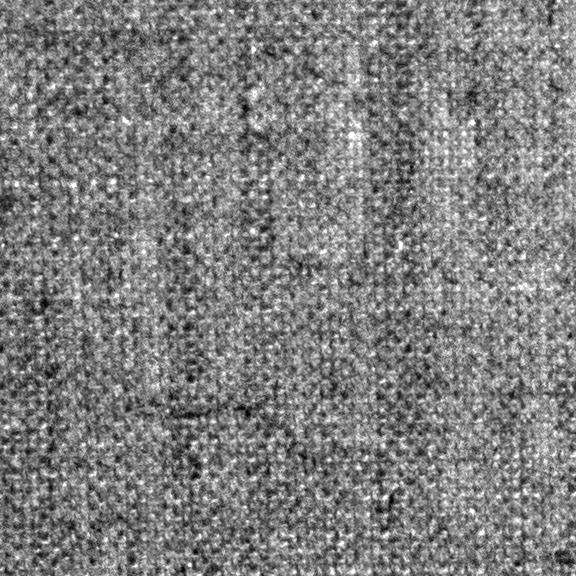
\includegraphics[width=.8\linewidth]{kylberg_examples/canvas1_003.png}
  %\caption{V-measure digits 2 and 9}
%  \label{fig:sfig2}
\end{subfigure}
\begin{subfigure}{.15\textwidth}
  \centering
  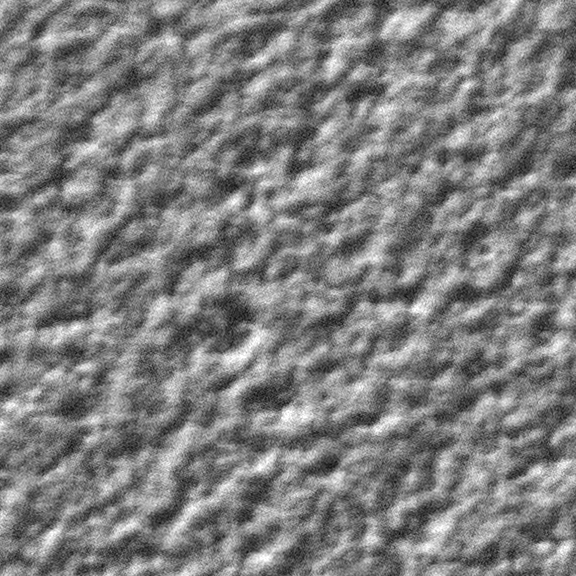
\includegraphics[width=.8\linewidth]{kylberg_examples/ceiling1_003.png}
  %\caption{PCA of digits 2 and 9}
 % \label{fig:sfig1}
\end{subfigure}%
\begin{subfigure}{.15\textwidth}
  \centering
  \includegraphics[width=.8\linewidth]{kylberg_examples/lentils1_003.png}
  %\caption{Purity digits 2 and 9}
%  \label{fig:sfig2}
\end{subfigure}
\begin{subfigure}{.15\textwidth}
  \centering
  \includegraphics[width=.8\linewidth]{kylberg_examples/screen1_003.png}
  %\caption{V-measure digits 2 and 9}
%  \label{fig:sfig2}
\end{subfigure}
\caption{Three examples from each of the 6 different texture tiles used in the streaming data set. The texture classes are (L-R) Blanket 1, Blanket 2, Canvas, Ceiling, Lentils and Screen}
\label{fig:texture_examples}
\end{figure}

The performance plots for the texture data are shown in Figure \ref{fig:texture_results}. Here we can see a difference between windowed spectral clustering and unweighted clustream, the windowed approach is generally performing better. Once again weighted clustream does not perform well, and performance seems to decline as the stream progresses.

\begin{figure}[h!]
\begin{subfigure}{.5\textwidth}
  \centering
  \includegraphics[width=1\linewidth]{texture_purity}
  \caption{Texture Purity}
 % \label{fig:sfig1}
\end{subfigure}%
\begin{subfigure}{.5\textwidth}
  \centering
  \includegraphics[width=1\linewidth]{texture_vmeasure}
  \caption{Texture V-measure}
%  \label{fig:sfig2}
\end{subfigure}
\caption{Texture Results}
\label{fig:texture_results}
\end{figure}

\subsection{Optional Extras}

\begin{itemize}
\item  Evaluate the number of micro-clusters needed for good performance. Give some insight into choosing the number of micro-clusters $q$. How does performance change based on the value of $q$? \cite{Aggarwal2003} suggests using the biggest value of $q$ computationally possible. I suspect diminishing returns when increasing $q$. Can I say something about this?
\item Show the distribution of micro-cluster sizes. Often it is very non-uniform, is it this which is effecting the performance of weighted spectral clustering?
\item Explain why Ning was not used in experimental results - too slow!
\end{itemize}

\subsubsection{Spectral Clustream vs Ning (without re-clustering)}
\label{sec:exp_ning}

In order to implement the Ning algorithm, the authors recommend a regular full re-clustering of the data sets to stop errors in the eigenvector estimates growing too large. 

In Figure \ref{fig:ning_no_reclust} I run both Ning and Clustream on the ``Norm overlap'' data set. We do not perform re-clustering for the Ning algorithm at all, so we can view how bad performance may get over time. 
This was run over a fairly short stream of just 200 data points. Cluster performance was requested every 10 time steps, resulting in 20 performance points. 

Although performance does seems to deteriorate over time, it isn't as dramatic as I expected. It would be nice to see this for a much longer stream (5000 data points?)

We can also see that Spectral Clustream is generally performing much better in terms of both purity and V-measure. It would be good to see something similar on real data. 

\begin{figure}[h!]
  \centering
  \includegraphics[width = 10cm]{ningNO_vs_clustream_norm_overlap_nMicro_50_length_200_batchSize_10.png}
  \caption{Ning (no re clustering) vs Spectral Clustream}
\label{fig:ning_no_reclust}
\end{figure}

However, I have found Ning very slow to run. The update method can be very expensive for fully connected networks, which makes it not feasible to use as it is in this study. However by using an $\epsilon$ neighbourhood to force the updates to be minimal I should be able to achieve a vast speed up. This will be tried on my return. I will also implement the regular re-clustering as recommended by the authors but this re-clustering will have to be over a window as it is not possible to performance a truly full re-clustering in a streaming setting.




 
\section{Conclusion}
\label{sec:micro_conc}

\begin{itemize}
\item The way to compare clustering algorithms in a streaming setting is not obvious
\item We may want a clustering to accurately represent the data stream in it's current state, however we may also wish to incorporate older stream information into the clustering.
\end{itemize}

%%%%%%%%%%%%%%%%%%%%%%%%%%%%%%%%%%%%%%%%%%%%%%%%%%%%%%%%%%%%%%%%%%%%%%%%%%%%
%%%%%%%%%%%%%%%%%%%%%%%%%%%%%%%%%%%%%%%%%%%%%%%%%%%%%%%%%%%%%%%%%%%%%%%%%%%%
% END OF CHAPTER
%%%%%%%%%%%%%%%%%%%%%%%%%%%%%%%%%%%%%%%%%%%%%%%%%%%%%%%%%%%%%%%%%%%%%%%%%%%%
%%%%%%%%%%%%%%%%%%%%%%%%%%%%%%%%%%%%%%%%%%%%%%%%%%%%%%%%%%%%%%%%%%%%%%%%%%%%

%---------------- COMMENT FOR IMPORTING ----------------------
% \pagebreak											%Comment for importing
% \bibliographystyle{apalike}		%Comment for importing
% \bibliography{/home/rhian/Dropbox/library,/home/rhian/Dropbox/rhian}
% \end{document}
% Comment for importing
%-------------------------------------------------------------

% \subsubsection{Clustream and evolving data sets - jump}

% We are also interested in evolving data sets. In this simple simulated data set, one cluster instantly jumps from one location to another. Figure \ref{fig:jump} shows performance of Clustream k-means and Clustream spectral on this jump detest. 
% \begin{figure}[h!]
%   \centering
%   \includegraphics[width = 8cm]{norm_jump_nMicro_150.png}
%   \caption{Clustream - jump data set}
% \label{fig:jump}
% \end{figure}



%%%%%%%%%%%%%%%%%%%%%%%%%%%%%%%%%%%%%%%%%%%%%%%%%%%%%%%%%%%%%%%%%%%%%%%%%%%%
% Information about the datasets
%%%%%%%%%%%%%%%%%%%%%%%%%%%%%%%%%%%%%%%%%%%%%%%%%%%%%%%%%%%%%%%%%%%%%%%%%%%%


% \subsection{Simulated data results}

% \begin{table}[h!]
% \centering
% \label{tab:sim_data}
% \begin{tabular}{lll}
% Data set & \# Dim & \# Clusters \\ \hline
% A       & 2      & 3           \\
% B       & 3      & 5           \\
% C       & 2      & 2           \\
% D       & 3      & 4           \\
% E       & 3      & 6           \\
% F       & 5      & 8          
% \end{tabular}
% \caption{Simulated Data sets}
% \end{table}

% If using, also introduce norm, norm overlap, t, cassini, spirals, norm jump. 



%%%%%%%%%%%%%%%%%%%%%%%%%%%%%%%%%%%%%%%%%%%%%%%%%%%%%%%%%%%%%%%%%%%%%%%%%%%%
%Extra (old) experimentation
%%%%%%%%%%%%%%%%%%%%%%%%%%%%%%%%%%%%%%%%%%%%%%%%%%%%%%%%%%%%%%%%%%%%%%%%%%%%


%\begin{figure}[h]
%  \centering
%  \includegraphics[width = 11cm]{nnSim.png}
%  \caption{When spectral clustering goes wrong - Neighborhood choice - not trivial!}
%\end{figure}


% \subsection{Stationary Datastreams}
% The online clustering is tested when datastream is stationary and non-stationary. Firstly we consider the stationary case. In this setting, the initial trial dataset includes some datapoints from each of the underlying clusters. Throughout the stream, datapoints from these initial clusters are generated. No clusters are removed, merge or join through the dataset. 
% Results are shown for two simulated datasets and one real image based dataset. Dataset A of 2 dimensions, 6 clusters and is normally correlated with uniform mean shift. Dataset B has 8 clusters, and 5 dimensions. Dataset C is  LS2W texture data taken from the Kylberg dataset. The Kylberg dataset is a texture database of many different images. I have used a subset of images from this set. The features come from L2SW decompostion for 7 levels in 3 directions - therefore 21 dimensions. I have found that LS2W representation is good at distinguishing between the different textures. 
% PCA plots of all three datasets can be seen in Figure .

% \begin{figure}
%   \centering
%   \includegraphics[width = 11cm]{set456.png}
%   \caption{Seed 456, 6 clusters, 2 dimensions - easy}  \label{fig:dataA}
% \end{figure}


% \begin{figure}[h]
%   \centering
%   \includegraphics[width = 11cm]{set420.png}
%   \caption{Seed 420, 8 clusters, 5 dimensions - medium} \label{fig:dataB}
% \end{figure}


% \begin{figure}[h]
%   \centering
%   \includegraphics[width = 11cm]{texturebatch.png}
%   \caption{Real texture data, tricker but too short?}
% \end{figure}

% Figure \ref{fig:dataA} shows performance and V-measure for Dataset A over runs of the data. The dataset consists of 60,000 datapoints, and the offline algorithms performed clustering every 1000 timesteps. 250 micro-clusteres were used to track the datastream. We can see that Kmeans generally performs poorly, jumping around 0.8. DBScan has a more consistant performance, hovering around 0.9. Spectral clustering performs very good segmentation throughout the trial, consistantly having values of 1 for purity and v-measure which corresponds to perfect clustering. We would expect to see this variability in kmeans due to the dependency on the initial seed points.

% Figure \ref{fig:dataB} shows performance and V-measure for Dataset B over runs of the data. The dataset consists of 80,000 datapoints, and the offline algorithms performed clustering every 1000 timesteps. 250 micro-clusteres were used to track the datastream. We can see that Kmeans generally performs poorly, jumping around 0.8. DBScan has a more consistant performance, hovering around 0.9. Spectral clustering performs perfrect clustering in 52/60 of the clusterings which occasionally drops to 0.9. 

% \subsection{Non-stationary Datastreams}

% Tracking micro-clusters for non-stationary datastreams brings an additional challenge. Underlying clustering may vanish over time, or move , or new clusters can join. Interesting challenges include succesfully detecting between an outlier of an existing cluster, and the start of a new emereging cluster. 


% \subsection{Time improvement against offline methods}

% Offline spectral clustering. This is standard spectral clustering algorithm performed on all of the most seen data up to time $t$, performed whenever $t$ is divisible by the batch size $b$. As this uses all of the datapoints it can produce very accurate results but is very slow to run. 

% Offline K-means. Standard kmeans, performed on all data up to time $t$ when $\frac{t}{b}$ divides exactly. Very quick but variable performance.

%%%%%%%%%%%%%%%%%%%%%%%%%%%%%%%%%%%%%%%%%%%%%%%%%%%%%%%%%%%%%%%%%%%%%%%%%%%%
%KASP BOUND INTRO  - redundent
%%%%%%%%%%%%%%%%%%%%%%%%%%%%%%%%%%%%%%%%%%%%%%%%%%%%%%%%%%%%%%%%%%%%%%%%%%%%

%\subsection{Performance Metrics}

% In order to investigate the performance of our algorithm we will assess it on both simulated and real data.  Standard offline spectral clustering will be compared against the streaming spectral clustering. The affinity matrix will be used as described in Section \ref{sec:spec}. V-measure and purity will be used to interpret cluster performance, and specifically a misclustering rate will be used to compare directly against the offline case.  

% introduces the misclustering rate to quantify the difference between an original and perturbed dataset described as 
% \begin{equation}
%   \label{eq:misClust}
%   \rho = \frac{1}{n} \sum_{i = 1}^{n} \mathbb{I}(I_i \neq \tilde{I}_i)
% \end{equation}

% Here $\mathbb{I}$ is the indicator function, $I_i$ represents the cluster allocated to original datapoint $x_i$ and $\tilde{I_i}$ represents the cluster allocation of perturbed datapoint $\tilde{x}_i$. If $\rho = 1$ then the clustering of the perturbed data is identical to the clustering of the original data. In Section \ref{sec:bounds} we will attempt to justify bounds on the values of the misclustering $\rho$ given some understanding of the micro-clustering process used.

% To compute purity , each cluster is assigned to the class which is most frequent in the cluster, and then the accuracy of this assignment is measured by counting the number of correctly assigned documents and dividing by $N$. Formally:
% \begin{equation}
% \mbox{purity}(\Omega,C) = \frac{1}{N} \sum_k \max_j \vert \omega_k \cap c_j\vert
% \end{equation} 	
% where $\Omega = \{ \omega_1, \omega_2, \ldots, \omega_K \}$is the set of clusters and $C = \{ c_1,c_2,\ldots,c_J \}$ is the set of classes Bad clusterings have purity values close to 0, a perfect clustering has a purity of 1 .Purity can become very high when there are a large number f clusters and therefore there it is not suitable for all cases, despite its nice simplicity. The V-Measure (A. Rosenberg and J. Hirschberg, 2007.) is described the harmonic mean of the homogenity and the completeness. This allows. Both these measures will allow us to compare the overall performance of the clustering given we know the ideal clustering scenario. However when working online with massive datasets we may be h
% appy to just get a performance as good as or as close to the offline performance as possible

% \section{Theoretical Guarantees and Bounds}
% \label{sec:bounds}
% Aim is to investigate the impact of clustering performance of perturbation on the data. The data perturbation is modelled as noisy observations. 

% $\tilde{x_i} = x_i + \epsilon_i$

% KASP investigated the relationship between data perturbation and the misclutering rate $\rho$ and determined a link between the perturbation on the Laplacian matrices and $\rho$, which is reprinted here. 

% Assume that: 1) the assumptions of Theorem 1(list) hold throughout the recursive invocation of the Ncut algorithm, 2) the smallest eigengap
% $g_0$ along the recursion is bounded away from zero, and 3) the Frobenius norm of the perturbation on Laplacian matrices along the recursion is bounded by $c\|\tilde{L} - L\|_F^2$ for some constant $c \geq 1$. Then the mis-clustering rate for an m-way spectral clustering solution can be  BOUNDED BY

% \BEGIN{EQUATION}
%   \LABEL{EQ:KASPTHM3}
%   \rho \leq \frac{m}{g_0^2} \cdot c \| \tilde{L} - L \|_F^2.
% \end{equation}

% This provides a link between the perturbation of the original dataset and the perturbation of the Laplacian matrix. 


